% The \phantomsection command is needed to create a link to a place in the document that is not a
% figure, equation, table, section, subsection, chapter, etc.
% https://tex.stackexchange.com/questions/44088/when-do-i-need-to-invoke-phantomsection
\phantomsection

% Multiple-language document - babel - selectlanguage vs begin/end{otherlanguage}
% https://tex.stackexchange.com/questions/36526/multiple-language-document-babel-selectlanguage-vs-begin-endotherlanguage
\begin{otherlanguage*}{english}

% Generated by eval/scripts/write_thesis_results_latex_assets.py. Figure macros only; result tables are inlined in chapters/results.tex.

\newcommand{\AsrHeatmapFigure}{%
\begin{figure}[htbp]
\centering
\scriptsize
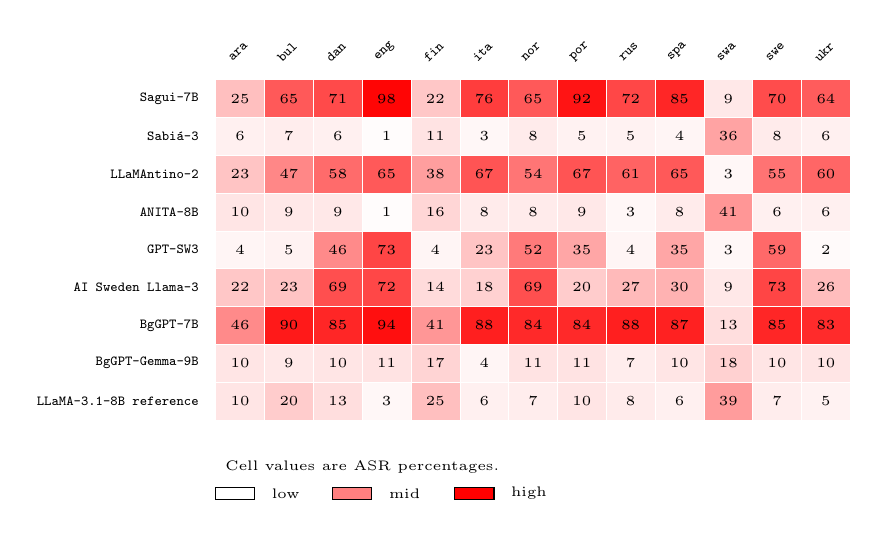
\begin{tikzpicture}[x=0.62cm,y=0.48cm]
\node[rotate=45,anchor=west,font=\tiny] at (0.16,0.35) {\texttt{ara}};
\node[rotate=45,anchor=west,font=\tiny] at (1.16,0.35) {\texttt{bul}};
\node[rotate=45,anchor=west,font=\tiny] at (2.16,0.35) {\texttt{dan}};
\node[rotate=45,anchor=west,font=\tiny] at (3.16,0.35) {\texttt{eng}};
\node[rotate=45,anchor=west,font=\tiny] at (4.16,0.35) {\texttt{fin}};
\node[rotate=45,anchor=west,font=\tiny] at (5.16,0.35) {\texttt{ita}};
\node[rotate=45,anchor=west,font=\tiny] at (6.16,0.35) {\texttt{nor}};
\node[rotate=45,anchor=west,font=\tiny] at (7.16,0.35) {\texttt{por}};
\node[rotate=45,anchor=west,font=\tiny] at (8.16,0.35) {\texttt{rus}};
\node[rotate=45,anchor=west,font=\tiny] at (9.16,0.35) {\texttt{spa}};
\node[rotate=45,anchor=west,font=\tiny] at (10.16,0.35) {\texttt{swa}};
\node[rotate=45,anchor=west,font=\tiny] at (11.16,0.35) {\texttt{swe}};
\node[rotate=45,anchor=west,font=\tiny] at (12.16,0.35) {\texttt{ukr}};
\node[anchor=east,font=\tiny] at (-0.15,-0.5) {\texttt{Sagui-7B}};
\fill[red!25!white] (0,0) rectangle ++(1,-1);
\draw[white,line width=0.2pt] (0,0) rectangle ++(1,-1);
\node[font=\tiny] at (0.5,-0.5) {25};
\fill[red!65!white] (1,0) rectangle ++(1,-1);
\draw[white,line width=0.2pt] (1,0) rectangle ++(1,-1);
\node[font=\tiny] at (1.5,-0.5) {65};
\fill[red!71!white] (2,0) rectangle ++(1,-1);
\draw[white,line width=0.2pt] (2,0) rectangle ++(1,-1);
\node[font=\tiny] at (2.5,-0.5) {71};
\fill[red!98!white] (3,0) rectangle ++(1,-1);
\draw[white,line width=0.2pt] (3,0) rectangle ++(1,-1);
\node[font=\tiny] at (3.5,-0.5) {98};
\fill[red!22!white] (4,0) rectangle ++(1,-1);
\draw[white,line width=0.2pt] (4,0) rectangle ++(1,-1);
\node[font=\tiny] at (4.5,-0.5) {22};
\fill[red!76!white] (5,0) rectangle ++(1,-1);
\draw[white,line width=0.2pt] (5,0) rectangle ++(1,-1);
\node[font=\tiny] at (5.5,-0.5) {76};
\fill[red!65!white] (6,0) rectangle ++(1,-1);
\draw[white,line width=0.2pt] (6,0) rectangle ++(1,-1);
\node[font=\tiny] at (6.5,-0.5) {65};
\fill[red!92!white] (7,0) rectangle ++(1,-1);
\draw[white,line width=0.2pt] (7,0) rectangle ++(1,-1);
\node[font=\tiny] at (7.5,-0.5) {92};
\fill[red!72!white] (8,0) rectangle ++(1,-1);
\draw[white,line width=0.2pt] (8,0) rectangle ++(1,-1);
\node[font=\tiny] at (8.5,-0.5) {72};
\fill[red!85!white] (9,0) rectangle ++(1,-1);
\draw[white,line width=0.2pt] (9,0) rectangle ++(1,-1);
\node[font=\tiny] at (9.5,-0.5) {85};
\fill[red!9!white] (10,0) rectangle ++(1,-1);
\draw[white,line width=0.2pt] (10,0) rectangle ++(1,-1);
\node[font=\tiny] at (10.5,-0.5) {9};
\fill[red!70!white] (11,0) rectangle ++(1,-1);
\draw[white,line width=0.2pt] (11,0) rectangle ++(1,-1);
\node[font=\tiny] at (11.5,-0.5) {70};
\fill[red!64!white] (12,0) rectangle ++(1,-1);
\draw[white,line width=0.2pt] (12,0) rectangle ++(1,-1);
\node[font=\tiny] at (12.5,-0.5) {64};
\node[anchor=east,font=\tiny] at (-0.15,-1.5) {\texttt{Sabi\'a-3}};
\fill[red!6!white] (0,-1) rectangle ++(1,-1);
\draw[white,line width=0.2pt] (0,-1) rectangle ++(1,-1);
\node[font=\tiny] at (0.5,-1.5) {6};
\fill[red!7!white] (1,-1) rectangle ++(1,-1);
\draw[white,line width=0.2pt] (1,-1) rectangle ++(1,-1);
\node[font=\tiny] at (1.5,-1.5) {7};
\fill[red!6!white] (2,-1) rectangle ++(1,-1);
\draw[white,line width=0.2pt] (2,-1) rectangle ++(1,-1);
\node[font=\tiny] at (2.5,-1.5) {6};
\fill[red!1!white] (3,-1) rectangle ++(1,-1);
\draw[white,line width=0.2pt] (3,-1) rectangle ++(1,-1);
\node[font=\tiny] at (3.5,-1.5) {1};
\fill[red!11!white] (4,-1) rectangle ++(1,-1);
\draw[white,line width=0.2pt] (4,-1) rectangle ++(1,-1);
\node[font=\tiny] at (4.5,-1.5) {11};
\fill[red!3!white] (5,-1) rectangle ++(1,-1);
\draw[white,line width=0.2pt] (5,-1) rectangle ++(1,-1);
\node[font=\tiny] at (5.5,-1.5) {3};
\fill[red!8!white] (6,-1) rectangle ++(1,-1);
\draw[white,line width=0.2pt] (6,-1) rectangle ++(1,-1);
\node[font=\tiny] at (6.5,-1.5) {8};
\fill[red!5!white] (7,-1) rectangle ++(1,-1);
\draw[white,line width=0.2pt] (7,-1) rectangle ++(1,-1);
\node[font=\tiny] at (7.5,-1.5) {5};
\fill[red!5!white] (8,-1) rectangle ++(1,-1);
\draw[white,line width=0.2pt] (8,-1) rectangle ++(1,-1);
\node[font=\tiny] at (8.5,-1.5) {5};
\fill[red!4!white] (9,-1) rectangle ++(1,-1);
\draw[white,line width=0.2pt] (9,-1) rectangle ++(1,-1);
\node[font=\tiny] at (9.5,-1.5) {4};
\fill[red!36!white] (10,-1) rectangle ++(1,-1);
\draw[white,line width=0.2pt] (10,-1) rectangle ++(1,-1);
\node[font=\tiny] at (10.5,-1.5) {36};
\fill[red!8!white] (11,-1) rectangle ++(1,-1);
\draw[white,line width=0.2pt] (11,-1) rectangle ++(1,-1);
\node[font=\tiny] at (11.5,-1.5) {8};
\fill[red!6!white] (12,-1) rectangle ++(1,-1);
\draw[white,line width=0.2pt] (12,-1) rectangle ++(1,-1);
\node[font=\tiny] at (12.5,-1.5) {6};
\node[anchor=east,font=\tiny] at (-0.15,-2.5) {\texttt{LLaMAntino-2}};
\fill[red!23!white] (0,-2) rectangle ++(1,-1);
\draw[white,line width=0.2pt] (0,-2) rectangle ++(1,-1);
\node[font=\tiny] at (0.5,-2.5) {23};
\fill[red!47!white] (1,-2) rectangle ++(1,-1);
\draw[white,line width=0.2pt] (1,-2) rectangle ++(1,-1);
\node[font=\tiny] at (1.5,-2.5) {47};
\fill[red!58!white] (2,-2) rectangle ++(1,-1);
\draw[white,line width=0.2pt] (2,-2) rectangle ++(1,-1);
\node[font=\tiny] at (2.5,-2.5) {58};
\fill[red!65!white] (3,-2) rectangle ++(1,-1);
\draw[white,line width=0.2pt] (3,-2) rectangle ++(1,-1);
\node[font=\tiny] at (3.5,-2.5) {65};
\fill[red!38!white] (4,-2) rectangle ++(1,-1);
\draw[white,line width=0.2pt] (4,-2) rectangle ++(1,-1);
\node[font=\tiny] at (4.5,-2.5) {38};
\fill[red!67!white] (5,-2) rectangle ++(1,-1);
\draw[white,line width=0.2pt] (5,-2) rectangle ++(1,-1);
\node[font=\tiny] at (5.5,-2.5) {67};
\fill[red!54!white] (6,-2) rectangle ++(1,-1);
\draw[white,line width=0.2pt] (6,-2) rectangle ++(1,-1);
\node[font=\tiny] at (6.5,-2.5) {54};
\fill[red!67!white] (7,-2) rectangle ++(1,-1);
\draw[white,line width=0.2pt] (7,-2) rectangle ++(1,-1);
\node[font=\tiny] at (7.5,-2.5) {67};
\fill[red!61!white] (8,-2) rectangle ++(1,-1);
\draw[white,line width=0.2pt] (8,-2) rectangle ++(1,-1);
\node[font=\tiny] at (8.5,-2.5) {61};
\fill[red!65!white] (9,-2) rectangle ++(1,-1);
\draw[white,line width=0.2pt] (9,-2) rectangle ++(1,-1);
\node[font=\tiny] at (9.5,-2.5) {65};
\fill[red!3!white] (10,-2) rectangle ++(1,-1);
\draw[white,line width=0.2pt] (10,-2) rectangle ++(1,-1);
\node[font=\tiny] at (10.5,-2.5) {3};
\fill[red!55!white] (11,-2) rectangle ++(1,-1);
\draw[white,line width=0.2pt] (11,-2) rectangle ++(1,-1);
\node[font=\tiny] at (11.5,-2.5) {55};
\fill[red!60!white] (12,-2) rectangle ++(1,-1);
\draw[white,line width=0.2pt] (12,-2) rectangle ++(1,-1);
\node[font=\tiny] at (12.5,-2.5) {60};
\node[anchor=east,font=\tiny] at (-0.15,-3.5) {\texttt{ANITA-8B}};
\fill[red!10!white] (0,-3) rectangle ++(1,-1);
\draw[white,line width=0.2pt] (0,-3) rectangle ++(1,-1);
\node[font=\tiny] at (0.5,-3.5) {10};
\fill[red!9!white] (1,-3) rectangle ++(1,-1);
\draw[white,line width=0.2pt] (1,-3) rectangle ++(1,-1);
\node[font=\tiny] at (1.5,-3.5) {9};
\fill[red!9!white] (2,-3) rectangle ++(1,-1);
\draw[white,line width=0.2pt] (2,-3) rectangle ++(1,-1);
\node[font=\tiny] at (2.5,-3.5) {9};
\fill[red!1!white] (3,-3) rectangle ++(1,-1);
\draw[white,line width=0.2pt] (3,-3) rectangle ++(1,-1);
\node[font=\tiny] at (3.5,-3.5) {1};
\fill[red!16!white] (4,-3) rectangle ++(1,-1);
\draw[white,line width=0.2pt] (4,-3) rectangle ++(1,-1);
\node[font=\tiny] at (4.5,-3.5) {16};
\fill[red!8!white] (5,-3) rectangle ++(1,-1);
\draw[white,line width=0.2pt] (5,-3) rectangle ++(1,-1);
\node[font=\tiny] at (5.5,-3.5) {8};
\fill[red!8!white] (6,-3) rectangle ++(1,-1);
\draw[white,line width=0.2pt] (6,-3) rectangle ++(1,-1);
\node[font=\tiny] at (6.5,-3.5) {8};
\fill[red!9!white] (7,-3) rectangle ++(1,-1);
\draw[white,line width=0.2pt] (7,-3) rectangle ++(1,-1);
\node[font=\tiny] at (7.5,-3.5) {9};
\fill[red!3!white] (8,-3) rectangle ++(1,-1);
\draw[white,line width=0.2pt] (8,-3) rectangle ++(1,-1);
\node[font=\tiny] at (8.5,-3.5) {3};
\fill[red!8!white] (9,-3) rectangle ++(1,-1);
\draw[white,line width=0.2pt] (9,-3) rectangle ++(1,-1);
\node[font=\tiny] at (9.5,-3.5) {8};
\fill[red!41!white] (10,-3) rectangle ++(1,-1);
\draw[white,line width=0.2pt] (10,-3) rectangle ++(1,-1);
\node[font=\tiny] at (10.5,-3.5) {41};
\fill[red!6!white] (11,-3) rectangle ++(1,-1);
\draw[white,line width=0.2pt] (11,-3) rectangle ++(1,-1);
\node[font=\tiny] at (11.5,-3.5) {6};
\fill[red!6!white] (12,-3) rectangle ++(1,-1);
\draw[white,line width=0.2pt] (12,-3) rectangle ++(1,-1);
\node[font=\tiny] at (12.5,-3.5) {6};
\node[anchor=east,font=\tiny] at (-0.15,-4.5) {\texttt{GPT-SW3}};
\fill[red!4!white] (0,-4) rectangle ++(1,-1);
\draw[white,line width=0.2pt] (0,-4) rectangle ++(1,-1);
\node[font=\tiny] at (0.5,-4.5) {4};
\fill[red!5!white] (1,-4) rectangle ++(1,-1);
\draw[white,line width=0.2pt] (1,-4) rectangle ++(1,-1);
\node[font=\tiny] at (1.5,-4.5) {5};
\fill[red!46!white] (2,-4) rectangle ++(1,-1);
\draw[white,line width=0.2pt] (2,-4) rectangle ++(1,-1);
\node[font=\tiny] at (2.5,-4.5) {46};
\fill[red!73!white] (3,-4) rectangle ++(1,-1);
\draw[white,line width=0.2pt] (3,-4) rectangle ++(1,-1);
\node[font=\tiny] at (3.5,-4.5) {73};
\fill[red!4!white] (4,-4) rectangle ++(1,-1);
\draw[white,line width=0.2pt] (4,-4) rectangle ++(1,-1);
\node[font=\tiny] at (4.5,-4.5) {4};
\fill[red!23!white] (5,-4) rectangle ++(1,-1);
\draw[white,line width=0.2pt] (5,-4) rectangle ++(1,-1);
\node[font=\tiny] at (5.5,-4.5) {23};
\fill[red!52!white] (6,-4) rectangle ++(1,-1);
\draw[white,line width=0.2pt] (6,-4) rectangle ++(1,-1);
\node[font=\tiny] at (6.5,-4.5) {52};
\fill[red!35!white] (7,-4) rectangle ++(1,-1);
\draw[white,line width=0.2pt] (7,-4) rectangle ++(1,-1);
\node[font=\tiny] at (7.5,-4.5) {35};
\fill[red!4!white] (8,-4) rectangle ++(1,-1);
\draw[white,line width=0.2pt] (8,-4) rectangle ++(1,-1);
\node[font=\tiny] at (8.5,-4.5) {4};
\fill[red!35!white] (9,-4) rectangle ++(1,-1);
\draw[white,line width=0.2pt] (9,-4) rectangle ++(1,-1);
\node[font=\tiny] at (9.5,-4.5) {35};
\fill[red!3!white] (10,-4) rectangle ++(1,-1);
\draw[white,line width=0.2pt] (10,-4) rectangle ++(1,-1);
\node[font=\tiny] at (10.5,-4.5) {3};
\fill[red!59!white] (11,-4) rectangle ++(1,-1);
\draw[white,line width=0.2pt] (11,-4) rectangle ++(1,-1);
\node[font=\tiny] at (11.5,-4.5) {59};
\fill[red!2!white] (12,-4) rectangle ++(1,-1);
\draw[white,line width=0.2pt] (12,-4) rectangle ++(1,-1);
\node[font=\tiny] at (12.5,-4.5) {2};
\node[anchor=east,font=\tiny] at (-0.15,-5.5) {\texttt{AI Sweden Llama-3}};
\fill[red!22!white] (0,-5) rectangle ++(1,-1);
\draw[white,line width=0.2pt] (0,-5) rectangle ++(1,-1);
\node[font=\tiny] at (0.5,-5.5) {22};
\fill[red!23!white] (1,-5) rectangle ++(1,-1);
\draw[white,line width=0.2pt] (1,-5) rectangle ++(1,-1);
\node[font=\tiny] at (1.5,-5.5) {23};
\fill[red!69!white] (2,-5) rectangle ++(1,-1);
\draw[white,line width=0.2pt] (2,-5) rectangle ++(1,-1);
\node[font=\tiny] at (2.5,-5.5) {69};
\fill[red!72!white] (3,-5) rectangle ++(1,-1);
\draw[white,line width=0.2pt] (3,-5) rectangle ++(1,-1);
\node[font=\tiny] at (3.5,-5.5) {72};
\fill[red!14!white] (4,-5) rectangle ++(1,-1);
\draw[white,line width=0.2pt] (4,-5) rectangle ++(1,-1);
\node[font=\tiny] at (4.5,-5.5) {14};
\fill[red!18!white] (5,-5) rectangle ++(1,-1);
\draw[white,line width=0.2pt] (5,-5) rectangle ++(1,-1);
\node[font=\tiny] at (5.5,-5.5) {18};
\fill[red!69!white] (6,-5) rectangle ++(1,-1);
\draw[white,line width=0.2pt] (6,-5) rectangle ++(1,-1);
\node[font=\tiny] at (6.5,-5.5) {69};
\fill[red!20!white] (7,-5) rectangle ++(1,-1);
\draw[white,line width=0.2pt] (7,-5) rectangle ++(1,-1);
\node[font=\tiny] at (7.5,-5.5) {20};
\fill[red!27!white] (8,-5) rectangle ++(1,-1);
\draw[white,line width=0.2pt] (8,-5) rectangle ++(1,-1);
\node[font=\tiny] at (8.5,-5.5) {27};
\fill[red!30!white] (9,-5) rectangle ++(1,-1);
\draw[white,line width=0.2pt] (9,-5) rectangle ++(1,-1);
\node[font=\tiny] at (9.5,-5.5) {30};
\fill[red!9!white] (10,-5) rectangle ++(1,-1);
\draw[white,line width=0.2pt] (10,-5) rectangle ++(1,-1);
\node[font=\tiny] at (10.5,-5.5) {9};
\fill[red!73!white] (11,-5) rectangle ++(1,-1);
\draw[white,line width=0.2pt] (11,-5) rectangle ++(1,-1);
\node[font=\tiny] at (11.5,-5.5) {73};
\fill[red!26!white] (12,-5) rectangle ++(1,-1);
\draw[white,line width=0.2pt] (12,-5) rectangle ++(1,-1);
\node[font=\tiny] at (12.5,-5.5) {26};
\node[anchor=east,font=\tiny] at (-0.15,-6.5) {\texttt{BgGPT-7B}};
\fill[red!46!white] (0,-6) rectangle ++(1,-1);
\draw[white,line width=0.2pt] (0,-6) rectangle ++(1,-1);
\node[font=\tiny] at (0.5,-6.5) {46};
\fill[red!90!white] (1,-6) rectangle ++(1,-1);
\draw[white,line width=0.2pt] (1,-6) rectangle ++(1,-1);
\node[font=\tiny] at (1.5,-6.5) {90};
\fill[red!85!white] (2,-6) rectangle ++(1,-1);
\draw[white,line width=0.2pt] (2,-6) rectangle ++(1,-1);
\node[font=\tiny] at (2.5,-6.5) {85};
\fill[red!94!white] (3,-6) rectangle ++(1,-1);
\draw[white,line width=0.2pt] (3,-6) rectangle ++(1,-1);
\node[font=\tiny] at (3.5,-6.5) {94};
\fill[red!41!white] (4,-6) rectangle ++(1,-1);
\draw[white,line width=0.2pt] (4,-6) rectangle ++(1,-1);
\node[font=\tiny] at (4.5,-6.5) {41};
\fill[red!88!white] (5,-6) rectangle ++(1,-1);
\draw[white,line width=0.2pt] (5,-6) rectangle ++(1,-1);
\node[font=\tiny] at (5.5,-6.5) {88};
\fill[red!84!white] (6,-6) rectangle ++(1,-1);
\draw[white,line width=0.2pt] (6,-6) rectangle ++(1,-1);
\node[font=\tiny] at (6.5,-6.5) {84};
\fill[red!84!white] (7,-6) rectangle ++(1,-1);
\draw[white,line width=0.2pt] (7,-6) rectangle ++(1,-1);
\node[font=\tiny] at (7.5,-6.5) {84};
\fill[red!88!white] (8,-6) rectangle ++(1,-1);
\draw[white,line width=0.2pt] (8,-6) rectangle ++(1,-1);
\node[font=\tiny] at (8.5,-6.5) {88};
\fill[red!87!white] (9,-6) rectangle ++(1,-1);
\draw[white,line width=0.2pt] (9,-6) rectangle ++(1,-1);
\node[font=\tiny] at (9.5,-6.5) {87};
\fill[red!13!white] (10,-6) rectangle ++(1,-1);
\draw[white,line width=0.2pt] (10,-6) rectangle ++(1,-1);
\node[font=\tiny] at (10.5,-6.5) {13};
\fill[red!85!white] (11,-6) rectangle ++(1,-1);
\draw[white,line width=0.2pt] (11,-6) rectangle ++(1,-1);
\node[font=\tiny] at (11.5,-6.5) {85};
\fill[red!83!white] (12,-6) rectangle ++(1,-1);
\draw[white,line width=0.2pt] (12,-6) rectangle ++(1,-1);
\node[font=\tiny] at (12.5,-6.5) {83};
\node[anchor=east,font=\tiny] at (-0.15,-7.5) {\texttt{BgGPT-Gemma-9B}};
\fill[red!10!white] (0,-7) rectangle ++(1,-1);
\draw[white,line width=0.2pt] (0,-7) rectangle ++(1,-1);
\node[font=\tiny] at (0.5,-7.5) {10};
\fill[red!9!white] (1,-7) rectangle ++(1,-1);
\draw[white,line width=0.2pt] (1,-7) rectangle ++(1,-1);
\node[font=\tiny] at (1.5,-7.5) {9};
\fill[red!10!white] (2,-7) rectangle ++(1,-1);
\draw[white,line width=0.2pt] (2,-7) rectangle ++(1,-1);
\node[font=\tiny] at (2.5,-7.5) {10};
\fill[red!11!white] (3,-7) rectangle ++(1,-1);
\draw[white,line width=0.2pt] (3,-7) rectangle ++(1,-1);
\node[font=\tiny] at (3.5,-7.5) {11};
\fill[red!17!white] (4,-7) rectangle ++(1,-1);
\draw[white,line width=0.2pt] (4,-7) rectangle ++(1,-1);
\node[font=\tiny] at (4.5,-7.5) {17};
\fill[red!4!white] (5,-7) rectangle ++(1,-1);
\draw[white,line width=0.2pt] (5,-7) rectangle ++(1,-1);
\node[font=\tiny] at (5.5,-7.5) {4};
\fill[red!11!white] (6,-7) rectangle ++(1,-1);
\draw[white,line width=0.2pt] (6,-7) rectangle ++(1,-1);
\node[font=\tiny] at (6.5,-7.5) {11};
\fill[red!11!white] (7,-7) rectangle ++(1,-1);
\draw[white,line width=0.2pt] (7,-7) rectangle ++(1,-1);
\node[font=\tiny] at (7.5,-7.5) {11};
\fill[red!7!white] (8,-7) rectangle ++(1,-1);
\draw[white,line width=0.2pt] (8,-7) rectangle ++(1,-1);
\node[font=\tiny] at (8.5,-7.5) {7};
\fill[red!10!white] (9,-7) rectangle ++(1,-1);
\draw[white,line width=0.2pt] (9,-7) rectangle ++(1,-1);
\node[font=\tiny] at (9.5,-7.5) {10};
\fill[red!18!white] (10,-7) rectangle ++(1,-1);
\draw[white,line width=0.2pt] (10,-7) rectangle ++(1,-1);
\node[font=\tiny] at (10.5,-7.5) {18};
\fill[red!10!white] (11,-7) rectangle ++(1,-1);
\draw[white,line width=0.2pt] (11,-7) rectangle ++(1,-1);
\node[font=\tiny] at (11.5,-7.5) {10};
\fill[red!10!white] (12,-7) rectangle ++(1,-1);
\draw[white,line width=0.2pt] (12,-7) rectangle ++(1,-1);
\node[font=\tiny] at (12.5,-7.5) {10};
\node[anchor=east,font=\tiny] at (-0.15,-8.5) {\texttt{LLaMA-3.1-8B reference}};
\fill[red!10!white] (0,-8) rectangle ++(1,-1);
\draw[white,line width=0.2pt] (0,-8) rectangle ++(1,-1);
\node[font=\tiny] at (0.5,-8.5) {10};
\fill[red!20!white] (1,-8) rectangle ++(1,-1);
\draw[white,line width=0.2pt] (1,-8) rectangle ++(1,-1);
\node[font=\tiny] at (1.5,-8.5) {20};
\fill[red!13!white] (2,-8) rectangle ++(1,-1);
\draw[white,line width=0.2pt] (2,-8) rectangle ++(1,-1);
\node[font=\tiny] at (2.5,-8.5) {13};
\fill[red!3!white] (3,-8) rectangle ++(1,-1);
\draw[white,line width=0.2pt] (3,-8) rectangle ++(1,-1);
\node[font=\tiny] at (3.5,-8.5) {3};
\fill[red!25!white] (4,-8) rectangle ++(1,-1);
\draw[white,line width=0.2pt] (4,-8) rectangle ++(1,-1);
\node[font=\tiny] at (4.5,-8.5) {25};
\fill[red!6!white] (5,-8) rectangle ++(1,-1);
\draw[white,line width=0.2pt] (5,-8) rectangle ++(1,-1);
\node[font=\tiny] at (5.5,-8.5) {6};
\fill[red!7!white] (6,-8) rectangle ++(1,-1);
\draw[white,line width=0.2pt] (6,-8) rectangle ++(1,-1);
\node[font=\tiny] at (6.5,-8.5) {7};
\fill[red!10!white] (7,-8) rectangle ++(1,-1);
\draw[white,line width=0.2pt] (7,-8) rectangle ++(1,-1);
\node[font=\tiny] at (7.5,-8.5) {10};
\fill[red!8!white] (8,-8) rectangle ++(1,-1);
\draw[white,line width=0.2pt] (8,-8) rectangle ++(1,-1);
\node[font=\tiny] at (8.5,-8.5) {8};
\fill[red!6!white] (9,-8) rectangle ++(1,-1);
\draw[white,line width=0.2pt] (9,-8) rectangle ++(1,-1);
\node[font=\tiny] at (9.5,-8.5) {6};
\fill[red!39!white] (10,-8) rectangle ++(1,-1);
\draw[white,line width=0.2pt] (10,-8) rectangle ++(1,-1);
\node[font=\tiny] at (10.5,-8.5) {39};
\fill[red!7!white] (11,-8) rectangle ++(1,-1);
\draw[white,line width=0.2pt] (11,-8) rectangle ++(1,-1);
\node[font=\tiny] at (11.5,-8.5) {7};
\fill[red!5!white] (12,-8) rectangle ++(1,-1);
\draw[white,line width=0.2pt] (12,-8) rectangle ++(1,-1);
\node[font=\tiny] at (12.5,-8.5) {5};
\node[anchor=west,font=\tiny] at (0,-10.25) {Cell values are ASR percentages.};
\fill[red!0!white] (0,-10.8) rectangle ++(0.8,-0.3);\draw (0,-10.8) rectangle ++(0.8,-0.3);\node[anchor=west,font=\tiny] at (0.95,-10.950000000000001) {low};
\fill[red!50!white] (2.4,-10.8) rectangle ++(0.8,-0.3);\draw (2.4,-10.8) rectangle ++(0.8,-0.3);\node[anchor=west,font=\tiny] at (3.35,-10.950000000000001) {mid};
\fill[red!100!white] (4.9,-10.8) rectangle ++(0.8,-0.3);\draw (4.9,-10.8) rectangle ++(0.8,-0.3);\node[anchor=west,font=\tiny] at (5.85,-10.950000000000001) {high};
\end{tikzpicture}
\caption[ASR by model and attack language]{ASR by model and attack language.}
\label{fig:asr-heatmap}
\fonte{Author.}
\end{figure}
}

\newcommand{\DistanceAsrFigure}{%
\begin{figure}[htbp]
\centering
\begin{minipage}{0.48\linewidth}\centering
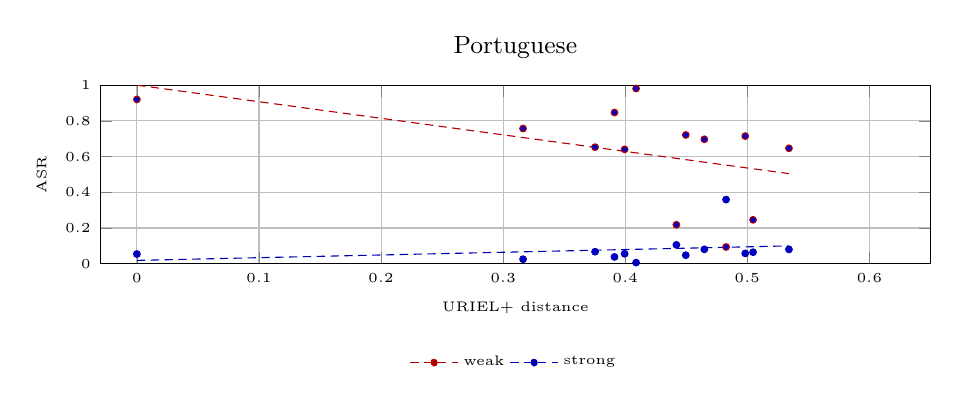
\begin{tikzpicture}
\begin{axis}[width=\linewidth,height=3.85cm,grid=both,
title={Portuguese},xlabel={URIEL+ distance},ylabel={ASR},
xmin=-0.03,xmax=0.65,ymin=0,ymax=1,
tick label style={font=\tiny},label style={font=\tiny},title style={font=\small},
legend style={font=\tiny,at={(0.5,-0.45)},anchor=north,draw=none,fill=none,legend columns=2}]
\addplot+[forget plot,only marks,mark=*,mark size=1.2pt,red!70!black] coordinates {(0.5047,0.2460) (0.3753,0.6527) (0.4983,0.7147) (0.4089,0.9808) (0.4419,0.2184) (0.3163,0.7572) (0.5341,0.6463) (0.0000,0.9199) (0.4496,0.7212) (0.3912,0.8466) (0.4826,0.0939) (0.4648,0.6968) (0.3995,0.6403)};
\addplot+[forget plot,no markers,densely dashed,red!70!black] coordinates {(0.0000,1.0000) (0.5341,0.5045)};
\addplot+[forget plot,only marks,mark=*,mark size=1.2pt,blue!70!black] coordinates {(0.5047,0.0647) (0.3753,0.0675) (0.4983,0.0581) (0.4089,0.0064) (0.4419,0.1058) (0.3163,0.0256) (0.5341,0.0804) (0.0000,0.0545) (0.4496,0.0481) (0.3912,0.0383) (0.4826,0.3592) (0.4648,0.0806) (0.3995,0.0561)};
\addplot+[forget plot,no markers,densely dashed,blue!70!black] coordinates {(0.0000,0.0188) (0.5341,0.1000)};
\addlegendimage{densely dashed,mark=*,mark size=1.2pt,red!70!black}
\addlegendentry{weak}
\addlegendimage{densely dashed,mark=*,mark size=1.2pt,blue!70!black}
\addlegendentry{strong}
\end{axis}
\end{tikzpicture}
\end{minipage}
\hfill\begin{minipage}{0.48\linewidth}\centering
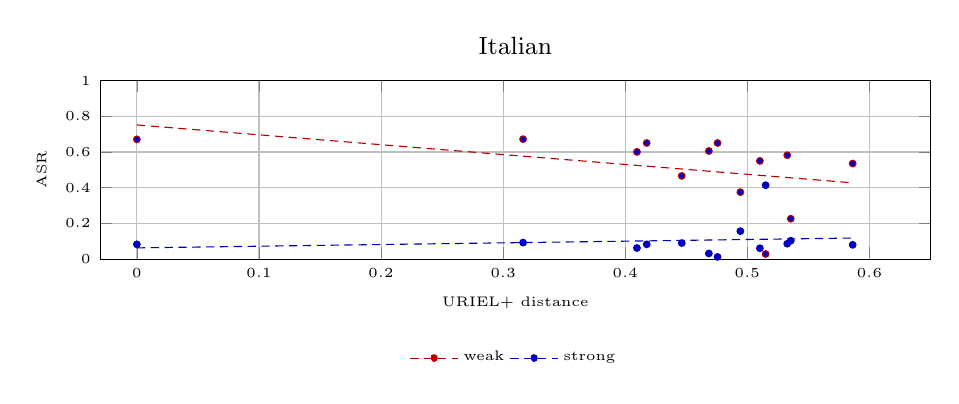
\begin{tikzpicture}
\begin{axis}[width=\linewidth,height=3.85cm,grid=both,
title={Italian},xlabel={URIEL+ distance},ylabel={ASR},
xmin=-0.03,xmax=0.65,ymin=0,ymax=1,
tick label style={font=\tiny},label style={font=\tiny},title style={font=\small},
legend style={font=\tiny,at={(0.5,-0.45)},anchor=north,draw=none,fill=none,legend columns=2}]
\addplot+[forget plot,only marks,mark=*,mark size=1.2pt,red!70!black] coordinates {(0.5356,0.2265) (0.4463,0.4662) (0.5327,0.5820) (0.4756,0.6506) (0.4943,0.3754) (0.0000,0.6709) (0.5863,0.5355) (0.3163,0.6720) (0.4685,0.6058) (0.4176,0.6506) (0.5150,0.0291) (0.5103,0.5502) (0.4096,0.6007)};
\addplot+[forget plot,no markers,densely dashed,red!70!black] coordinates {(0.0000,0.7516) (0.5863,0.4275)};
\addplot+[forget plot,only marks,mark=*,mark size=1.2pt,blue!70!black] coordinates {(0.5356,0.1036) (0.4463,0.0900) (0.5327,0.0865) (0.4756,0.0128) (0.4943,0.1570) (0.0000,0.0831) (0.5863,0.0804) (0.3163,0.0929) (0.4685,0.0321) (0.4176,0.0831) (0.5150,0.4142) (0.5103,0.0613) (0.4096,0.0627)};
\addplot+[forget plot,no markers,densely dashed,blue!70!black] coordinates {(0.0000,0.0633) (0.5863,0.1184)};
\addlegendimage{densely dashed,mark=*,mark size=1.2pt,red!70!black}
\addlegendentry{weak}
\addlegendimage{densely dashed,mark=*,mark size=1.2pt,blue!70!black}
\addlegendentry{strong}
\end{axis}
\end{tikzpicture}
\end{minipage}
\vspace{0.7cm}
\begin{minipage}{0.48\linewidth}\centering
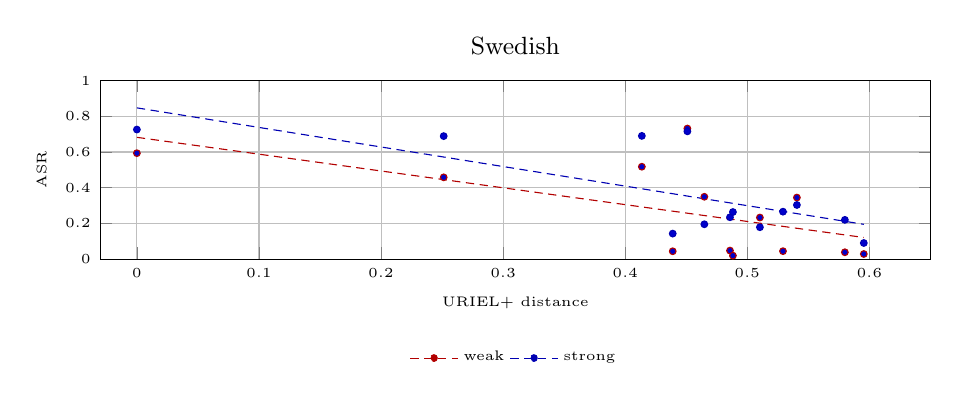
\begin{tikzpicture}
\begin{axis}[width=\linewidth,height=3.85cm,grid=both,
title={Swedish},xlabel={URIEL+ distance},ylabel={ASR},
xmin=-0.03,xmax=0.65,ymin=0,ymax=1,
tick label style={font=\tiny},label style={font=\tiny},title style={font=\small},
legend style={font=\tiny,at={(0.5,-0.45)},anchor=north,draw=none,fill=none,legend columns=2}]
\addplot+[forget plot,only marks,mark=*,mark size=1.2pt,red!70!black] coordinates {(0.5799,0.0388) (0.4858,0.0482) (0.2513,0.4583) (0.4509,0.7316) (0.4389,0.0444) (0.5103,0.2332) (0.4136,0.5177) (0.4648,0.3494) (0.5292,0.0449) (0.5406,0.3450) (0.5954,0.0291) (0.0000,0.5935) (0.4882,0.0198)};
\addplot+[forget plot,no markers,densely dashed,red!70!black] coordinates {(0.0000,0.6822) (0.5954,0.1214)};
\addplot+[forget plot,only marks,mark=*,mark size=1.2pt,blue!70!black] coordinates {(0.5799,0.2201) (0.4858,0.2347) (0.2513,0.6891) (0.4509,0.7157) (0.4389,0.1433) (0.5103,0.1789) (0.4136,0.6903) (0.4648,0.1955) (0.5292,0.2660) (0.5406,0.3035) (0.5954,0.0906) (0.0000,0.7258) (0.4882,0.2640)};
\addplot+[forget plot,no markers,densely dashed,blue!70!black] coordinates {(0.0000,0.8472) (0.5954,0.1952)};
\addlegendimage{densely dashed,mark=*,mark size=1.2pt,red!70!black}
\addlegendentry{weak}
\addlegendimage{densely dashed,mark=*,mark size=1.2pt,blue!70!black}
\addlegendentry{strong}
\end{axis}
\end{tikzpicture}
\end{minipage}
\hfill\begin{minipage}{0.48\linewidth}\centering
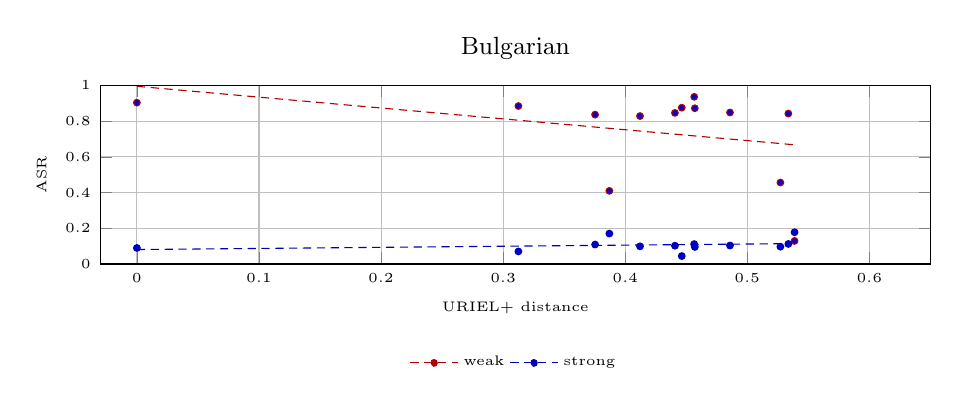
\begin{tikzpicture}
\begin{axis}[width=\linewidth,height=3.85cm,grid=both,
title={Bulgarian},xlabel={URIEL+ distance},ylabel={ASR},
xmin=-0.03,xmax=0.65,ymin=0,ymax=1,
tick label style={font=\tiny},label style={font=\tiny},title style={font=\small},
legend style={font=\tiny,at={(0.5,-0.45)},anchor=north,draw=none,fill=none,legend columns=2}]
\addplot+[forget plot,only marks,mark=*,mark size=1.2pt,red!70!black] coordinates {(0.5271,0.4563) (0.0000,0.9035) (0.4407,0.8462) (0.4565,0.9361) (0.3870,0.4096) (0.4463,0.8754) (0.5336,0.8424) (0.3753,0.8365) (0.3125,0.8846) (0.4570,0.8722) (0.5387,0.1294) (0.4858,0.8484) (0.4121,0.8284)};
\addplot+[forget plot,no markers,densely dashed,red!70!black] coordinates {(0.0000,0.9952) (0.5387,0.6675)};
\addplot+[forget plot,only marks,mark=*,mark size=1.2pt,blue!70!black] coordinates {(0.5271,0.0971) (0.0000,0.0900) (0.4407,0.1026) (0.4565,0.1118) (0.3870,0.1706) (0.4463,0.0447) (0.5336,0.1125) (0.3753,0.1090) (0.3125,0.0705) (0.4570,0.0958) (0.5387,0.1780) (0.4858,0.1037) (0.4121,0.0990)};
\addplot+[forget plot,no markers,densely dashed,blue!70!black] coordinates {(0.0000,0.0810) (0.5387,0.1144)};
\addlegendimage{densely dashed,mark=*,mark size=1.2pt,red!70!black}
\addlegendentry{weak}
\addlegendimage{densely dashed,mark=*,mark size=1.2pt,blue!70!black}
\addlegendentry{strong}
\end{axis}
\end{tikzpicture}
\end{minipage}
\vspace{0.7cm}
\begin{minipage}{0.48\linewidth}\centering
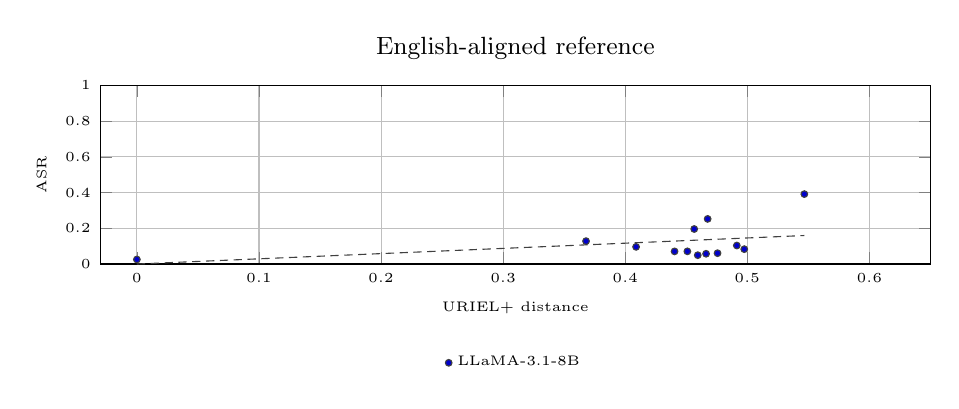
\begin{tikzpicture}
\begin{axis}[width=\linewidth,height=3.85cm,grid=both,
title={English-aligned reference},xlabel={URIEL+ distance},ylabel={ASR},
xmin=-0.03,xmax=0.65,ymin=0,ymax=1,
tick label style={font=\tiny},label style={font=\tiny},title style={font=\small},
legend style={font=\tiny,at={(0.5,-0.45)},anchor=north,draw=none,fill=none}]
\addplot+[only marks,mark=*,mark size=1.2pt,black!75!white] coordinates {(0.4914,0.1036) (0.4565,0.1961) (0.3679,0.1282) (0.0000,0.0256) (0.4675,0.2526) (0.4756,0.0607) (0.4404,0.0707) (0.4089,0.0962) (0.4975,0.0833) (0.4662,0.0575) (0.5467,0.3916) (0.4509,0.0710) (0.4594,0.0495)};
\addlegendentry{LLaMA-3.1-8B}
\addplot+[no markers,densely dashed,black!75!white] coordinates {(0.0000,0.0000) (0.5467,0.1596)};
\end{axis}
\end{tikzpicture}
\end{minipage}
\caption[Language-risk curves relating ASR to URIEL+ distance]{Language-risk curves relating ASR to URIEL+ distance.}
\label{fig:distance-vs-asr}
\fonte{Author.}
\end{figure}
}

\newcommand{\BelebeleIfHeatmapFigure}{%
\begin{figure}[htbp]
\centering
\scriptsize
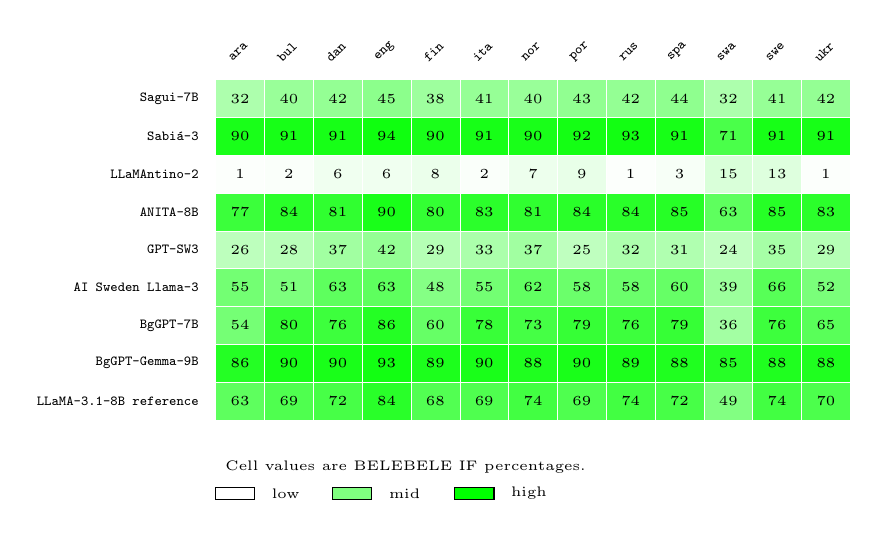
\begin{tikzpicture}[x=0.62cm,y=0.48cm]
\node[rotate=45,anchor=west,font=\tiny] at (0.16,0.35) {\texttt{ara}};
\node[rotate=45,anchor=west,font=\tiny] at (1.16,0.35) {\texttt{bul}};
\node[rotate=45,anchor=west,font=\tiny] at (2.16,0.35) {\texttt{dan}};
\node[rotate=45,anchor=west,font=\tiny] at (3.16,0.35) {\texttt{eng}};
\node[rotate=45,anchor=west,font=\tiny] at (4.16,0.35) {\texttt{fin}};
\node[rotate=45,anchor=west,font=\tiny] at (5.16,0.35) {\texttt{ita}};
\node[rotate=45,anchor=west,font=\tiny] at (6.16,0.35) {\texttt{nor}};
\node[rotate=45,anchor=west,font=\tiny] at (7.16,0.35) {\texttt{por}};
\node[rotate=45,anchor=west,font=\tiny] at (8.16,0.35) {\texttt{rus}};
\node[rotate=45,anchor=west,font=\tiny] at (9.16,0.35) {\texttt{spa}};
\node[rotate=45,anchor=west,font=\tiny] at (10.16,0.35) {\texttt{swa}};
\node[rotate=45,anchor=west,font=\tiny] at (11.16,0.35) {\texttt{swe}};
\node[rotate=45,anchor=west,font=\tiny] at (12.16,0.35) {\texttt{ukr}};
\node[anchor=east,font=\tiny] at (-0.15,-0.5) {\texttt{Sagui-7B}};
\fill[green!32!white] (0,0) rectangle ++(1,-1);
\draw[white,line width=0.2pt] (0,0) rectangle ++(1,-1);
\node[font=\tiny] at (0.5,-0.5) {32};
\fill[green!40!white] (1,0) rectangle ++(1,-1);
\draw[white,line width=0.2pt] (1,0) rectangle ++(1,-1);
\node[font=\tiny] at (1.5,-0.5) {40};
\fill[green!42!white] (2,0) rectangle ++(1,-1);
\draw[white,line width=0.2pt] (2,0) rectangle ++(1,-1);
\node[font=\tiny] at (2.5,-0.5) {42};
\fill[green!45!white] (3,0) rectangle ++(1,-1);
\draw[white,line width=0.2pt] (3,0) rectangle ++(1,-1);
\node[font=\tiny] at (3.5,-0.5) {45};
\fill[green!38!white] (4,0) rectangle ++(1,-1);
\draw[white,line width=0.2pt] (4,0) rectangle ++(1,-1);
\node[font=\tiny] at (4.5,-0.5) {38};
\fill[green!41!white] (5,0) rectangle ++(1,-1);
\draw[white,line width=0.2pt] (5,0) rectangle ++(1,-1);
\node[font=\tiny] at (5.5,-0.5) {41};
\fill[green!40!white] (6,0) rectangle ++(1,-1);
\draw[white,line width=0.2pt] (6,0) rectangle ++(1,-1);
\node[font=\tiny] at (6.5,-0.5) {40};
\fill[green!43!white] (7,0) rectangle ++(1,-1);
\draw[white,line width=0.2pt] (7,0) rectangle ++(1,-1);
\node[font=\tiny] at (7.5,-0.5) {43};
\fill[green!42!white] (8,0) rectangle ++(1,-1);
\draw[white,line width=0.2pt] (8,0) rectangle ++(1,-1);
\node[font=\tiny] at (8.5,-0.5) {42};
\fill[green!44!white] (9,0) rectangle ++(1,-1);
\draw[white,line width=0.2pt] (9,0) rectangle ++(1,-1);
\node[font=\tiny] at (9.5,-0.5) {44};
\fill[green!32!white] (10,0) rectangle ++(1,-1);
\draw[white,line width=0.2pt] (10,0) rectangle ++(1,-1);
\node[font=\tiny] at (10.5,-0.5) {32};
\fill[green!41!white] (11,0) rectangle ++(1,-1);
\draw[white,line width=0.2pt] (11,0) rectangle ++(1,-1);
\node[font=\tiny] at (11.5,-0.5) {41};
\fill[green!42!white] (12,0) rectangle ++(1,-1);
\draw[white,line width=0.2pt] (12,0) rectangle ++(1,-1);
\node[font=\tiny] at (12.5,-0.5) {42};
\node[anchor=east,font=\tiny] at (-0.15,-1.5) {\texttt{Sabi\'a-3}};
\fill[green!90!white] (0,-1) rectangle ++(1,-1);
\draw[white,line width=0.2pt] (0,-1) rectangle ++(1,-1);
\node[font=\tiny] at (0.5,-1.5) {90};
\fill[green!91!white] (1,-1) rectangle ++(1,-1);
\draw[white,line width=0.2pt] (1,-1) rectangle ++(1,-1);
\node[font=\tiny] at (1.5,-1.5) {91};
\fill[green!91!white] (2,-1) rectangle ++(1,-1);
\draw[white,line width=0.2pt] (2,-1) rectangle ++(1,-1);
\node[font=\tiny] at (2.5,-1.5) {91};
\fill[green!94!white] (3,-1) rectangle ++(1,-1);
\draw[white,line width=0.2pt] (3,-1) rectangle ++(1,-1);
\node[font=\tiny] at (3.5,-1.5) {94};
\fill[green!90!white] (4,-1) rectangle ++(1,-1);
\draw[white,line width=0.2pt] (4,-1) rectangle ++(1,-1);
\node[font=\tiny] at (4.5,-1.5) {90};
\fill[green!91!white] (5,-1) rectangle ++(1,-1);
\draw[white,line width=0.2pt] (5,-1) rectangle ++(1,-1);
\node[font=\tiny] at (5.5,-1.5) {91};
\fill[green!90!white] (6,-1) rectangle ++(1,-1);
\draw[white,line width=0.2pt] (6,-1) rectangle ++(1,-1);
\node[font=\tiny] at (6.5,-1.5) {90};
\fill[green!92!white] (7,-1) rectangle ++(1,-1);
\draw[white,line width=0.2pt] (7,-1) rectangle ++(1,-1);
\node[font=\tiny] at (7.5,-1.5) {92};
\fill[green!93!white] (8,-1) rectangle ++(1,-1);
\draw[white,line width=0.2pt] (8,-1) rectangle ++(1,-1);
\node[font=\tiny] at (8.5,-1.5) {93};
\fill[green!91!white] (9,-1) rectangle ++(1,-1);
\draw[white,line width=0.2pt] (9,-1) rectangle ++(1,-1);
\node[font=\tiny] at (9.5,-1.5) {91};
\fill[green!71!white] (10,-1) rectangle ++(1,-1);
\draw[white,line width=0.2pt] (10,-1) rectangle ++(1,-1);
\node[font=\tiny] at (10.5,-1.5) {71};
\fill[green!91!white] (11,-1) rectangle ++(1,-1);
\draw[white,line width=0.2pt] (11,-1) rectangle ++(1,-1);
\node[font=\tiny] at (11.5,-1.5) {91};
\fill[green!91!white] (12,-1) rectangle ++(1,-1);
\draw[white,line width=0.2pt] (12,-1) rectangle ++(1,-1);
\node[font=\tiny] at (12.5,-1.5) {91};
\node[anchor=east,font=\tiny] at (-0.15,-2.5) {\texttt{LLaMAntino-2}};
\fill[green!1!white] (0,-2) rectangle ++(1,-1);
\draw[white,line width=0.2pt] (0,-2) rectangle ++(1,-1);
\node[font=\tiny] at (0.5,-2.5) {1};
\fill[green!2!white] (1,-2) rectangle ++(1,-1);
\draw[white,line width=0.2pt] (1,-2) rectangle ++(1,-1);
\node[font=\tiny] at (1.5,-2.5) {2};
\fill[green!6!white] (2,-2) rectangle ++(1,-1);
\draw[white,line width=0.2pt] (2,-2) rectangle ++(1,-1);
\node[font=\tiny] at (2.5,-2.5) {6};
\fill[green!6!white] (3,-2) rectangle ++(1,-1);
\draw[white,line width=0.2pt] (3,-2) rectangle ++(1,-1);
\node[font=\tiny] at (3.5,-2.5) {6};
\fill[green!8!white] (4,-2) rectangle ++(1,-1);
\draw[white,line width=0.2pt] (4,-2) rectangle ++(1,-1);
\node[font=\tiny] at (4.5,-2.5) {8};
\fill[green!2!white] (5,-2) rectangle ++(1,-1);
\draw[white,line width=0.2pt] (5,-2) rectangle ++(1,-1);
\node[font=\tiny] at (5.5,-2.5) {2};
\fill[green!7!white] (6,-2) rectangle ++(1,-1);
\draw[white,line width=0.2pt] (6,-2) rectangle ++(1,-1);
\node[font=\tiny] at (6.5,-2.5) {7};
\fill[green!9!white] (7,-2) rectangle ++(1,-1);
\draw[white,line width=0.2pt] (7,-2) rectangle ++(1,-1);
\node[font=\tiny] at (7.5,-2.5) {9};
\fill[green!1!white] (8,-2) rectangle ++(1,-1);
\draw[white,line width=0.2pt] (8,-2) rectangle ++(1,-1);
\node[font=\tiny] at (8.5,-2.5) {1};
\fill[green!3!white] (9,-2) rectangle ++(1,-1);
\draw[white,line width=0.2pt] (9,-2) rectangle ++(1,-1);
\node[font=\tiny] at (9.5,-2.5) {3};
\fill[green!15!white] (10,-2) rectangle ++(1,-1);
\draw[white,line width=0.2pt] (10,-2) rectangle ++(1,-1);
\node[font=\tiny] at (10.5,-2.5) {15};
\fill[green!13!white] (11,-2) rectangle ++(1,-1);
\draw[white,line width=0.2pt] (11,-2) rectangle ++(1,-1);
\node[font=\tiny] at (11.5,-2.5) {13};
\fill[green!1!white] (12,-2) rectangle ++(1,-1);
\draw[white,line width=0.2pt] (12,-2) rectangle ++(1,-1);
\node[font=\tiny] at (12.5,-2.5) {1};
\node[anchor=east,font=\tiny] at (-0.15,-3.5) {\texttt{ANITA-8B}};
\fill[green!77!white] (0,-3) rectangle ++(1,-1);
\draw[white,line width=0.2pt] (0,-3) rectangle ++(1,-1);
\node[font=\tiny] at (0.5,-3.5) {77};
\fill[green!84!white] (1,-3) rectangle ++(1,-1);
\draw[white,line width=0.2pt] (1,-3) rectangle ++(1,-1);
\node[font=\tiny] at (1.5,-3.5) {84};
\fill[green!81!white] (2,-3) rectangle ++(1,-1);
\draw[white,line width=0.2pt] (2,-3) rectangle ++(1,-1);
\node[font=\tiny] at (2.5,-3.5) {81};
\fill[green!90!white] (3,-3) rectangle ++(1,-1);
\draw[white,line width=0.2pt] (3,-3) rectangle ++(1,-1);
\node[font=\tiny] at (3.5,-3.5) {90};
\fill[green!80!white] (4,-3) rectangle ++(1,-1);
\draw[white,line width=0.2pt] (4,-3) rectangle ++(1,-1);
\node[font=\tiny] at (4.5,-3.5) {80};
\fill[green!83!white] (5,-3) rectangle ++(1,-1);
\draw[white,line width=0.2pt] (5,-3) rectangle ++(1,-1);
\node[font=\tiny] at (5.5,-3.5) {83};
\fill[green!81!white] (6,-3) rectangle ++(1,-1);
\draw[white,line width=0.2pt] (6,-3) rectangle ++(1,-1);
\node[font=\tiny] at (6.5,-3.5) {81};
\fill[green!84!white] (7,-3) rectangle ++(1,-1);
\draw[white,line width=0.2pt] (7,-3) rectangle ++(1,-1);
\node[font=\tiny] at (7.5,-3.5) {84};
\fill[green!84!white] (8,-3) rectangle ++(1,-1);
\draw[white,line width=0.2pt] (8,-3) rectangle ++(1,-1);
\node[font=\tiny] at (8.5,-3.5) {84};
\fill[green!85!white] (9,-3) rectangle ++(1,-1);
\draw[white,line width=0.2pt] (9,-3) rectangle ++(1,-1);
\node[font=\tiny] at (9.5,-3.5) {85};
\fill[green!63!white] (10,-3) rectangle ++(1,-1);
\draw[white,line width=0.2pt] (10,-3) rectangle ++(1,-1);
\node[font=\tiny] at (10.5,-3.5) {63};
\fill[green!85!white] (11,-3) rectangle ++(1,-1);
\draw[white,line width=0.2pt] (11,-3) rectangle ++(1,-1);
\node[font=\tiny] at (11.5,-3.5) {85};
\fill[green!83!white] (12,-3) rectangle ++(1,-1);
\draw[white,line width=0.2pt] (12,-3) rectangle ++(1,-1);
\node[font=\tiny] at (12.5,-3.5) {83};
\node[anchor=east,font=\tiny] at (-0.15,-4.5) {\texttt{GPT-SW3}};
\fill[green!26!white] (0,-4) rectangle ++(1,-1);
\draw[white,line width=0.2pt] (0,-4) rectangle ++(1,-1);
\node[font=\tiny] at (0.5,-4.5) {26};
\fill[green!28!white] (1,-4) rectangle ++(1,-1);
\draw[white,line width=0.2pt] (1,-4) rectangle ++(1,-1);
\node[font=\tiny] at (1.5,-4.5) {28};
\fill[green!37!white] (2,-4) rectangle ++(1,-1);
\draw[white,line width=0.2pt] (2,-4) rectangle ++(1,-1);
\node[font=\tiny] at (2.5,-4.5) {37};
\fill[green!42!white] (3,-4) rectangle ++(1,-1);
\draw[white,line width=0.2pt] (3,-4) rectangle ++(1,-1);
\node[font=\tiny] at (3.5,-4.5) {42};
\fill[green!29!white] (4,-4) rectangle ++(1,-1);
\draw[white,line width=0.2pt] (4,-4) rectangle ++(1,-1);
\node[font=\tiny] at (4.5,-4.5) {29};
\fill[green!33!white] (5,-4) rectangle ++(1,-1);
\draw[white,line width=0.2pt] (5,-4) rectangle ++(1,-1);
\node[font=\tiny] at (5.5,-4.5) {33};
\fill[green!37!white] (6,-4) rectangle ++(1,-1);
\draw[white,line width=0.2pt] (6,-4) rectangle ++(1,-1);
\node[font=\tiny] at (6.5,-4.5) {37};
\fill[green!25!white] (7,-4) rectangle ++(1,-1);
\draw[white,line width=0.2pt] (7,-4) rectangle ++(1,-1);
\node[font=\tiny] at (7.5,-4.5) {25};
\fill[green!32!white] (8,-4) rectangle ++(1,-1);
\draw[white,line width=0.2pt] (8,-4) rectangle ++(1,-1);
\node[font=\tiny] at (8.5,-4.5) {32};
\fill[green!31!white] (9,-4) rectangle ++(1,-1);
\draw[white,line width=0.2pt] (9,-4) rectangle ++(1,-1);
\node[font=\tiny] at (9.5,-4.5) {31};
\fill[green!24!white] (10,-4) rectangle ++(1,-1);
\draw[white,line width=0.2pt] (10,-4) rectangle ++(1,-1);
\node[font=\tiny] at (10.5,-4.5) {24};
\fill[green!35!white] (11,-4) rectangle ++(1,-1);
\draw[white,line width=0.2pt] (11,-4) rectangle ++(1,-1);
\node[font=\tiny] at (11.5,-4.5) {35};
\fill[green!29!white] (12,-4) rectangle ++(1,-1);
\draw[white,line width=0.2pt] (12,-4) rectangle ++(1,-1);
\node[font=\tiny] at (12.5,-4.5) {29};
\node[anchor=east,font=\tiny] at (-0.15,-5.5) {\texttt{AI Sweden Llama-3}};
\fill[green!55!white] (0,-5) rectangle ++(1,-1);
\draw[white,line width=0.2pt] (0,-5) rectangle ++(1,-1);
\node[font=\tiny] at (0.5,-5.5) {55};
\fill[green!51!white] (1,-5) rectangle ++(1,-1);
\draw[white,line width=0.2pt] (1,-5) rectangle ++(1,-1);
\node[font=\tiny] at (1.5,-5.5) {51};
\fill[green!63!white] (2,-5) rectangle ++(1,-1);
\draw[white,line width=0.2pt] (2,-5) rectangle ++(1,-1);
\node[font=\tiny] at (2.5,-5.5) {63};
\fill[green!63!white] (3,-5) rectangle ++(1,-1);
\draw[white,line width=0.2pt] (3,-5) rectangle ++(1,-1);
\node[font=\tiny] at (3.5,-5.5) {63};
\fill[green!48!white] (4,-5) rectangle ++(1,-1);
\draw[white,line width=0.2pt] (4,-5) rectangle ++(1,-1);
\node[font=\tiny] at (4.5,-5.5) {48};
\fill[green!55!white] (5,-5) rectangle ++(1,-1);
\draw[white,line width=0.2pt] (5,-5) rectangle ++(1,-1);
\node[font=\tiny] at (5.5,-5.5) {55};
\fill[green!62!white] (6,-5) rectangle ++(1,-1);
\draw[white,line width=0.2pt] (6,-5) rectangle ++(1,-1);
\node[font=\tiny] at (6.5,-5.5) {62};
\fill[green!58!white] (7,-5) rectangle ++(1,-1);
\draw[white,line width=0.2pt] (7,-5) rectangle ++(1,-1);
\node[font=\tiny] at (7.5,-5.5) {58};
\fill[green!58!white] (8,-5) rectangle ++(1,-1);
\draw[white,line width=0.2pt] (8,-5) rectangle ++(1,-1);
\node[font=\tiny] at (8.5,-5.5) {58};
\fill[green!60!white] (9,-5) rectangle ++(1,-1);
\draw[white,line width=0.2pt] (9,-5) rectangle ++(1,-1);
\node[font=\tiny] at (9.5,-5.5) {60};
\fill[green!39!white] (10,-5) rectangle ++(1,-1);
\draw[white,line width=0.2pt] (10,-5) rectangle ++(1,-1);
\node[font=\tiny] at (10.5,-5.5) {39};
\fill[green!66!white] (11,-5) rectangle ++(1,-1);
\draw[white,line width=0.2pt] (11,-5) rectangle ++(1,-1);
\node[font=\tiny] at (11.5,-5.5) {66};
\fill[green!52!white] (12,-5) rectangle ++(1,-1);
\draw[white,line width=0.2pt] (12,-5) rectangle ++(1,-1);
\node[font=\tiny] at (12.5,-5.5) {52};
\node[anchor=east,font=\tiny] at (-0.15,-6.5) {\texttt{BgGPT-7B}};
\fill[green!54!white] (0,-6) rectangle ++(1,-1);
\draw[white,line width=0.2pt] (0,-6) rectangle ++(1,-1);
\node[font=\tiny] at (0.5,-6.5) {54};
\fill[green!80!white] (1,-6) rectangle ++(1,-1);
\draw[white,line width=0.2pt] (1,-6) rectangle ++(1,-1);
\node[font=\tiny] at (1.5,-6.5) {80};
\fill[green!76!white] (2,-6) rectangle ++(1,-1);
\draw[white,line width=0.2pt] (2,-6) rectangle ++(1,-1);
\node[font=\tiny] at (2.5,-6.5) {76};
\fill[green!86!white] (3,-6) rectangle ++(1,-1);
\draw[white,line width=0.2pt] (3,-6) rectangle ++(1,-1);
\node[font=\tiny] at (3.5,-6.5) {86};
\fill[green!60!white] (4,-6) rectangle ++(1,-1);
\draw[white,line width=0.2pt] (4,-6) rectangle ++(1,-1);
\node[font=\tiny] at (4.5,-6.5) {60};
\fill[green!78!white] (5,-6) rectangle ++(1,-1);
\draw[white,line width=0.2pt] (5,-6) rectangle ++(1,-1);
\node[font=\tiny] at (5.5,-6.5) {78};
\fill[green!73!white] (6,-6) rectangle ++(1,-1);
\draw[white,line width=0.2pt] (6,-6) rectangle ++(1,-1);
\node[font=\tiny] at (6.5,-6.5) {73};
\fill[green!79!white] (7,-6) rectangle ++(1,-1);
\draw[white,line width=0.2pt] (7,-6) rectangle ++(1,-1);
\node[font=\tiny] at (7.5,-6.5) {79};
\fill[green!76!white] (8,-6) rectangle ++(1,-1);
\draw[white,line width=0.2pt] (8,-6) rectangle ++(1,-1);
\node[font=\tiny] at (8.5,-6.5) {76};
\fill[green!79!white] (9,-6) rectangle ++(1,-1);
\draw[white,line width=0.2pt] (9,-6) rectangle ++(1,-1);
\node[font=\tiny] at (9.5,-6.5) {79};
\fill[green!36!white] (10,-6) rectangle ++(1,-1);
\draw[white,line width=0.2pt] (10,-6) rectangle ++(1,-1);
\node[font=\tiny] at (10.5,-6.5) {36};
\fill[green!76!white] (11,-6) rectangle ++(1,-1);
\draw[white,line width=0.2pt] (11,-6) rectangle ++(1,-1);
\node[font=\tiny] at (11.5,-6.5) {76};
\fill[green!65!white] (12,-6) rectangle ++(1,-1);
\draw[white,line width=0.2pt] (12,-6) rectangle ++(1,-1);
\node[font=\tiny] at (12.5,-6.5) {65};
\node[anchor=east,font=\tiny] at (-0.15,-7.5) {\texttt{BgGPT-Gemma-9B}};
\fill[green!86!white] (0,-7) rectangle ++(1,-1);
\draw[white,line width=0.2pt] (0,-7) rectangle ++(1,-1);
\node[font=\tiny] at (0.5,-7.5) {86};
\fill[green!90!white] (1,-7) rectangle ++(1,-1);
\draw[white,line width=0.2pt] (1,-7) rectangle ++(1,-1);
\node[font=\tiny] at (1.5,-7.5) {90};
\fill[green!90!white] (2,-7) rectangle ++(1,-1);
\draw[white,line width=0.2pt] (2,-7) rectangle ++(1,-1);
\node[font=\tiny] at (2.5,-7.5) {90};
\fill[green!93!white] (3,-7) rectangle ++(1,-1);
\draw[white,line width=0.2pt] (3,-7) rectangle ++(1,-1);
\node[font=\tiny] at (3.5,-7.5) {93};
\fill[green!89!white] (4,-7) rectangle ++(1,-1);
\draw[white,line width=0.2pt] (4,-7) rectangle ++(1,-1);
\node[font=\tiny] at (4.5,-7.5) {89};
\fill[green!90!white] (5,-7) rectangle ++(1,-1);
\draw[white,line width=0.2pt] (5,-7) rectangle ++(1,-1);
\node[font=\tiny] at (5.5,-7.5) {90};
\fill[green!88!white] (6,-7) rectangle ++(1,-1);
\draw[white,line width=0.2pt] (6,-7) rectangle ++(1,-1);
\node[font=\tiny] at (6.5,-7.5) {88};
\fill[green!90!white] (7,-7) rectangle ++(1,-1);
\draw[white,line width=0.2pt] (7,-7) rectangle ++(1,-1);
\node[font=\tiny] at (7.5,-7.5) {90};
\fill[green!89!white] (8,-7) rectangle ++(1,-1);
\draw[white,line width=0.2pt] (8,-7) rectangle ++(1,-1);
\node[font=\tiny] at (8.5,-7.5) {89};
\fill[green!88!white] (9,-7) rectangle ++(1,-1);
\draw[white,line width=0.2pt] (9,-7) rectangle ++(1,-1);
\node[font=\tiny] at (9.5,-7.5) {88};
\fill[green!85!white] (10,-7) rectangle ++(1,-1);
\draw[white,line width=0.2pt] (10,-7) rectangle ++(1,-1);
\node[font=\tiny] at (10.5,-7.5) {85};
\fill[green!88!white] (11,-7) rectangle ++(1,-1);
\draw[white,line width=0.2pt] (11,-7) rectangle ++(1,-1);
\node[font=\tiny] at (11.5,-7.5) {88};
\fill[green!88!white] (12,-7) rectangle ++(1,-1);
\draw[white,line width=0.2pt] (12,-7) rectangle ++(1,-1);
\node[font=\tiny] at (12.5,-7.5) {88};
\node[anchor=east,font=\tiny] at (-0.15,-8.5) {\texttt{LLaMA-3.1-8B reference}};
\fill[green!63!white] (0,-8) rectangle ++(1,-1);
\draw[white,line width=0.2pt] (0,-8) rectangle ++(1,-1);
\node[font=\tiny] at (0.5,-8.5) {63};
\fill[green!69!white] (1,-8) rectangle ++(1,-1);
\draw[white,line width=0.2pt] (1,-8) rectangle ++(1,-1);
\node[font=\tiny] at (1.5,-8.5) {69};
\fill[green!72!white] (2,-8) rectangle ++(1,-1);
\draw[white,line width=0.2pt] (2,-8) rectangle ++(1,-1);
\node[font=\tiny] at (2.5,-8.5) {72};
\fill[green!84!white] (3,-8) rectangle ++(1,-1);
\draw[white,line width=0.2pt] (3,-8) rectangle ++(1,-1);
\node[font=\tiny] at (3.5,-8.5) {84};
\fill[green!68!white] (4,-8) rectangle ++(1,-1);
\draw[white,line width=0.2pt] (4,-8) rectangle ++(1,-1);
\node[font=\tiny] at (4.5,-8.5) {68};
\fill[green!69!white] (5,-8) rectangle ++(1,-1);
\draw[white,line width=0.2pt] (5,-8) rectangle ++(1,-1);
\node[font=\tiny] at (5.5,-8.5) {69};
\fill[green!74!white] (6,-8) rectangle ++(1,-1);
\draw[white,line width=0.2pt] (6,-8) rectangle ++(1,-1);
\node[font=\tiny] at (6.5,-8.5) {74};
\fill[green!69!white] (7,-8) rectangle ++(1,-1);
\draw[white,line width=0.2pt] (7,-8) rectangle ++(1,-1);
\node[font=\tiny] at (7.5,-8.5) {69};
\fill[green!74!white] (8,-8) rectangle ++(1,-1);
\draw[white,line width=0.2pt] (8,-8) rectangle ++(1,-1);
\node[font=\tiny] at (8.5,-8.5) {74};
\fill[green!72!white] (9,-8) rectangle ++(1,-1);
\draw[white,line width=0.2pt] (9,-8) rectangle ++(1,-1);
\node[font=\tiny] at (9.5,-8.5) {72};
\fill[green!49!white] (10,-8) rectangle ++(1,-1);
\draw[white,line width=0.2pt] (10,-8) rectangle ++(1,-1);
\node[font=\tiny] at (10.5,-8.5) {49};
\fill[green!74!white] (11,-8) rectangle ++(1,-1);
\draw[white,line width=0.2pt] (11,-8) rectangle ++(1,-1);
\node[font=\tiny] at (11.5,-8.5) {74};
\fill[green!70!white] (12,-8) rectangle ++(1,-1);
\draw[white,line width=0.2pt] (12,-8) rectangle ++(1,-1);
\node[font=\tiny] at (12.5,-8.5) {70};
\node[anchor=west,font=\tiny] at (0,-10.25) {Cell values are BELEBELE IF percentages.};
\fill[green!0!white] (0,-10.8) rectangle ++(0.8,-0.3);\draw (0,-10.8) rectangle ++(0.8,-0.3);\node[anchor=west,font=\tiny] at (0.95,-10.950000000000001) {low};
\fill[green!50!white] (2.4,-10.8) rectangle ++(0.8,-0.3);\draw (2.4,-10.8) rectangle ++(0.8,-0.3);\node[anchor=west,font=\tiny] at (3.35,-10.950000000000001) {mid};
\fill[green!100!white] (4.9,-10.8) rectangle ++(0.8,-0.3);\draw (4.9,-10.8) rectangle ++(0.8,-0.3);\node[anchor=west,font=\tiny] at (5.85,-10.950000000000001) {high};
\end{tikzpicture}
\caption[BELEBELE IF score by model and attack language]{BELEBELE IF score by model and attack language.}
\label{fig:belebele-if-heatmap}
\fonte{Author.}
\end{figure}
}

\newcommand{\SpecAsrFigure}{%
\begin{figure}[htbp]
\centering
\begin{minipage}{0.48\linewidth}\centering
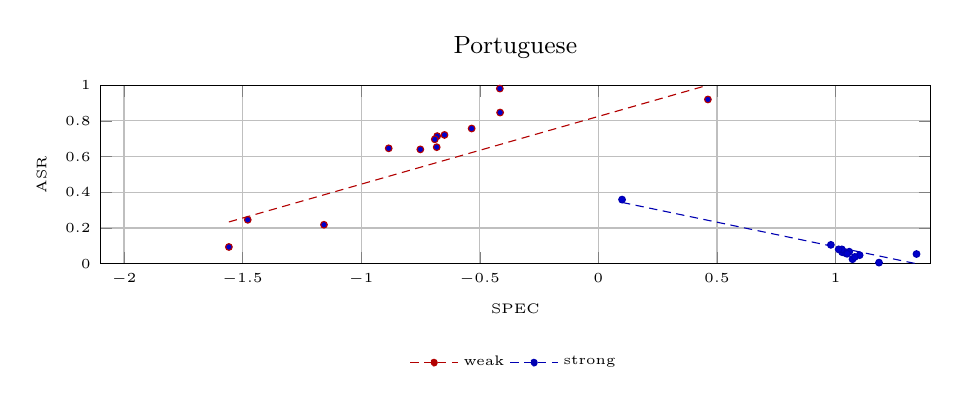
\begin{tikzpicture}
\begin{axis}[width=\linewidth,height=3.85cm,grid=both,
title={Portuguese},xlabel={SPEC},ylabel={ASR},
xmin=-2.1,xmax=1.4,ymin=0,ymax=1,
tick label style={font=\tiny},label style={font=\tiny},title style={font=\small},
legend style={font=\tiny,at={(0.5,-0.45)},anchor=north,draw=none,fill=none,legend columns=2}]
\addplot+[forget plot,only marks,mark=*,mark size=1.2pt,red!70!black] coordinates {(-1.4783,0.2460) (-0.6816,0.6527) (-0.6796,0.7147) (-0.4154,0.9808) (-1.1569,0.2184) (-0.5343,0.7572) (-0.8840,0.6463) (0.4617,0.9199) (-0.6488,0.7212) (-0.4143,0.8466) (-1.5577,0.0939) (-0.6897,0.6968) (-0.7506,0.6403)};
\addplot+[forget plot,no markers,densely dashed,red!70!black] coordinates {(-1.5577,0.2340) (0.4617,1.0000)};
\addplot+[forget plot,only marks,mark=*,mark size=1.2pt,blue!70!black] coordinates {(1.0279,0.0647) (1.0576,0.0675) (1.0442,0.0581) (1.1830,0.0064) (0.9800,0.1058) (1.0714,0.0256) (1.0266,0.0804) (1.3412,0.0545) (1.1013,0.0481) (1.0810,0.0383) (0.0998,0.3592) (1.0129,0.0806) (1.0490,0.0561)};
\addplot+[forget plot,no markers,densely dashed,blue!70!black] coordinates {(0.0998,0.3434) (1.3412,0.0000)};
\addlegendimage{densely dashed,mark=*,mark size=1.2pt,red!70!black}
\addlegendentry{weak}
\addlegendimage{densely dashed,mark=*,mark size=1.2pt,blue!70!black}
\addlegendentry{strong}
\end{axis}
\end{tikzpicture}
\end{minipage}
\hfill\begin{minipage}{0.48\linewidth}\centering
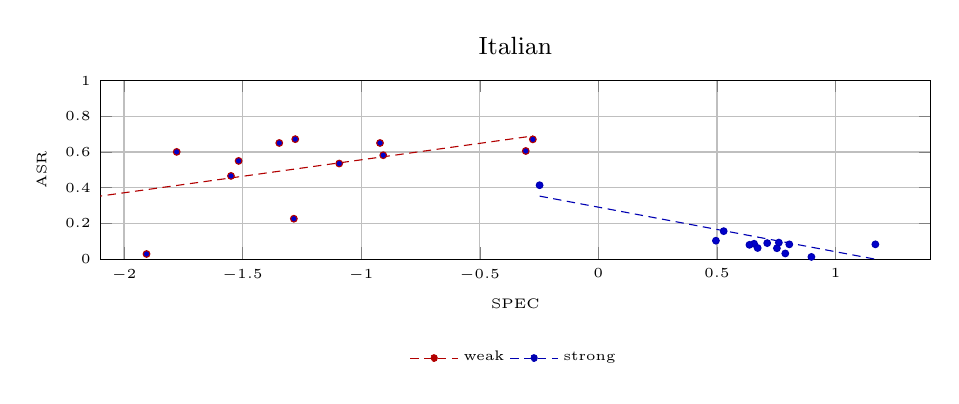
\begin{tikzpicture}
\begin{axis}[width=\linewidth,height=3.85cm,grid=both,
title={Italian},xlabel={SPEC},ylabel={ASR},
xmin=-2.1,xmax=1.4,ymin=0,ymax=1,
tick label style={font=\tiny},label style={font=\tiny},title style={font=\small},
legend style={font=\tiny,at={(0.5,-0.45)},anchor=north,draw=none,fill=none,legend columns=2}]
\addplot+[forget plot,only marks,mark=*,mark size=1.2pt,red!70!black] coordinates {(-1.2838,0.2265) (-1.5489,0.4662) (-0.9070,0.5820) (-0.9206,0.6506) (-2.1846,0.3754) (-0.2762,0.6709) (-1.0926,0.5355) (-1.2779,0.6720) (-0.3061,0.6058) (-1.3453,0.6506) (-1.9049,0.0291) (-1.5167,0.5502) (-1.7777,0.6007)};
\addplot+[forget plot,no markers,densely dashed,red!70!black] coordinates {(-2.1846,0.3377) (-0.2762,0.6899)};
\addplot+[forget plot,only marks,mark=*,mark size=1.2pt,blue!70!black] coordinates {(0.4955,0.1036) (0.7117,0.0900) (0.6564,0.0865) (0.8980,0.0128) (0.5282,0.1570) (1.1677,0.0831) (0.6368,0.0804) (0.7608,0.0929) (0.7879,0.0321) (0.8049,0.0831) (-0.2478,0.4142) (0.7526,0.0613) (0.6714,0.0627)};
\addplot+[forget plot,no markers,densely dashed,blue!70!black] coordinates {(-0.2478,0.3531) (1.1677,0.0000)};
\addlegendimage{densely dashed,mark=*,mark size=1.2pt,red!70!black}
\addlegendentry{weak}
\addlegendimage{densely dashed,mark=*,mark size=1.2pt,blue!70!black}
\addlegendentry{strong}
\end{axis}
\end{tikzpicture}
\end{minipage}
\vspace{0.7cm}
\begin{minipage}{0.48\linewidth}\centering
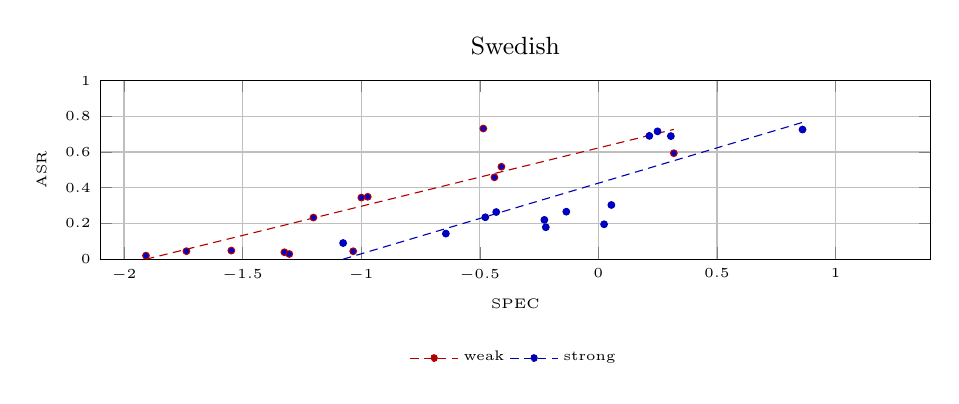
\begin{tikzpicture}
\begin{axis}[width=\linewidth,height=3.85cm,grid=both,
title={Swedish},xlabel={SPEC},ylabel={ASR},
xmin=-2.1,xmax=1.4,ymin=0,ymax=1,
tick label style={font=\tiny},label style={font=\tiny},title style={font=\small},
legend style={font=\tiny,at={(0.5,-0.45)},anchor=north,draw=none,fill=none,legend columns=2}]
\addplot+[forget plot,only marks,mark=*,mark size=1.2pt,red!70!black] coordinates {(-1.3237,0.0388) (-1.5474,0.0482) (-0.4383,0.4583) (-0.4850,0.7316) (-1.0337,0.0444) (-1.2013,0.2332) (-0.4087,0.5177) (-0.9724,0.3494) (-1.7367,0.0449) (-0.9992,0.3450) (-1.3031,0.0291) (0.3181,0.5935) (-1.9072,0.0198)};
\addplot+[forget plot,no markers,densely dashed,red!70!black] coordinates {(-1.9072,0.0000) (0.3181,0.7267)};
\addplot+[forget plot,only marks,mark=*,mark size=1.2pt,blue!70!black] coordinates {(-0.2277,0.2201) (-0.4768,0.2347) (0.3055,0.6891) (0.2493,0.7157) (-0.6430,0.1433) (-0.2216,0.1789) (0.2148,0.6903) (0.0240,0.1955) (-0.1352,0.2660) (0.0547,0.3035) (-1.0761,0.0906) (0.8606,0.7258) (-0.4307,0.2640)};
\addplot+[forget plot,no markers,densely dashed,blue!70!black] coordinates {(-1.0761,0.0000) (0.8606,0.7659)};
\addlegendimage{densely dashed,mark=*,mark size=1.2pt,red!70!black}
\addlegendentry{weak}
\addlegendimage{densely dashed,mark=*,mark size=1.2pt,blue!70!black}
\addlegendentry{strong}
\end{axis}
\end{tikzpicture}
\end{minipage}
\hfill\begin{minipage}{0.48\linewidth}\centering
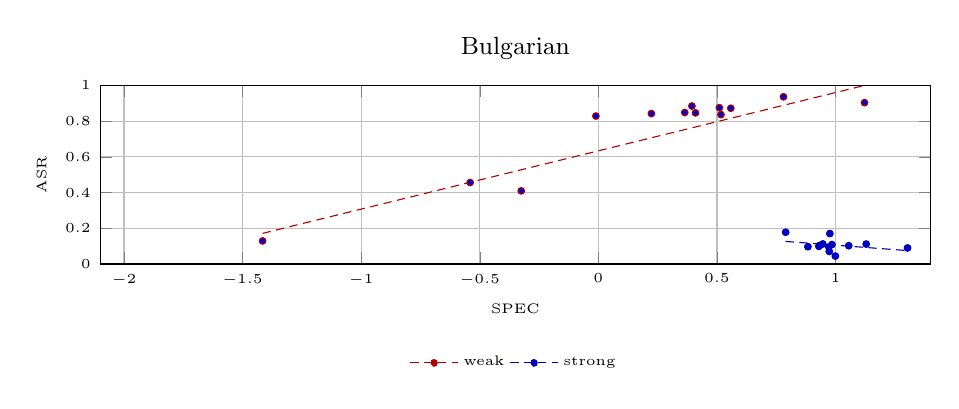
\begin{tikzpicture}
\begin{axis}[width=\linewidth,height=3.85cm,grid=both,
title={Bulgarian},xlabel={SPEC},ylabel={ASR},
xmin=-2.1,xmax=1.4,ymin=0,ymax=1,
tick label style={font=\tiny},label style={font=\tiny},title style={font=\small},
legend style={font=\tiny,at={(0.5,-0.45)},anchor=north,draw=none,fill=none,legend columns=2}]
\addplot+[forget plot,only marks,mark=*,mark size=1.2pt,red!70!black] coordinates {(-0.5405,0.4563) (1.1219,0.9035) (0.4094,0.8462) (0.7803,0.9361) (-0.3252,0.4096) (0.5102,0.8754) (0.2235,0.8424) (0.5168,0.8365) (0.3943,0.8846) (0.5583,0.8722) (-1.4156,0.1294) (0.3641,0.8484) (-0.0105,0.8284)};
\addplot+[forget plot,no markers,densely dashed,red!70!black] coordinates {(-1.4156,0.1718) (1.1219,1.0000)};
\addplot+[forget plot,only marks,mark=*,mark size=1.2pt,blue!70!black] coordinates {(0.8833,0.0971) (1.3034,0.0900) (1.0554,0.1026) (1.1290,0.1118) (0.9758,0.1706) (0.9990,0.0447) (0.9461,0.1125) (0.9845,0.1090) (0.9732,0.0705) (0.9711,0.0958) (0.7893,0.1780) (0.9323,0.1037) (0.9296,0.0990)};
\addplot+[forget plot,no markers,densely dashed,blue!70!black] coordinates {(0.7893,0.1267) (1.3034,0.0752)};
\addlegendimage{densely dashed,mark=*,mark size=1.2pt,red!70!black}
\addlegendentry{weak}
\addlegendimage{densely dashed,mark=*,mark size=1.2pt,blue!70!black}
\addlegendentry{strong}
\end{axis}
\end{tikzpicture}
\end{minipage}
\vspace{0.7cm}
\caption[ASR versus BELEBELE-derived specialization]{ASR versus BELEBELE-derived specialization.}
\label{fig:spec-vs-asr}
\fonte{Author.}
\end{figure}
}

\newcommand{\TokenizerDiagnosticsFigure}{%
\begin{figure}[htbp]
\centering
\scriptsize
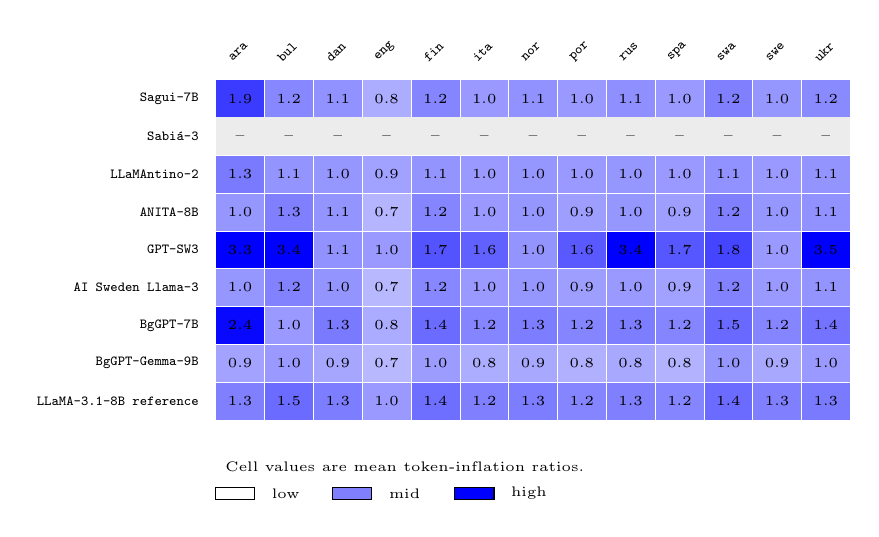
\begin{tikzpicture}[x=0.62cm,y=0.48cm]
\node[rotate=45,anchor=west,font=\tiny] at (0.16,0.35) {\texttt{ara}};
\node[rotate=45,anchor=west,font=\tiny] at (1.16,0.35) {\texttt{bul}};
\node[rotate=45,anchor=west,font=\tiny] at (2.16,0.35) {\texttt{dan}};
\node[rotate=45,anchor=west,font=\tiny] at (3.16,0.35) {\texttt{eng}};
\node[rotate=45,anchor=west,font=\tiny] at (4.16,0.35) {\texttt{fin}};
\node[rotate=45,anchor=west,font=\tiny] at (5.16,0.35) {\texttt{ita}};
\node[rotate=45,anchor=west,font=\tiny] at (6.16,0.35) {\texttt{nor}};
\node[rotate=45,anchor=west,font=\tiny] at (7.16,0.35) {\texttt{por}};
\node[rotate=45,anchor=west,font=\tiny] at (8.16,0.35) {\texttt{rus}};
\node[rotate=45,anchor=west,font=\tiny] at (9.16,0.35) {\texttt{spa}};
\node[rotate=45,anchor=west,font=\tiny] at (10.16,0.35) {\texttt{swa}};
\node[rotate=45,anchor=west,font=\tiny] at (11.16,0.35) {\texttt{swe}};
\node[rotate=45,anchor=west,font=\tiny] at (12.16,0.35) {\texttt{ukr}};
\node[anchor=east,font=\tiny] at (-0.15,-0.5) {\texttt{Sagui-7B}};
\fill[blue!77!white] (0,0) rectangle ++(1,-1);
\draw[white,line width=0.2pt] (0,0) rectangle ++(1,-1);
\node[font=\tiny] at (0.5,-0.5) {1.9};
\fill[blue!47!white] (1,0) rectangle ++(1,-1);
\draw[white,line width=0.2pt] (1,0) rectangle ++(1,-1);
\node[font=\tiny] at (1.5,-0.5) {1.2};
\fill[blue!43!white] (2,0) rectangle ++(1,-1);
\draw[white,line width=0.2pt] (2,0) rectangle ++(1,-1);
\node[font=\tiny] at (2.5,-0.5) {1.1};
\fill[blue!32!white] (3,0) rectangle ++(1,-1);
\draw[white,line width=0.2pt] (3,0) rectangle ++(1,-1);
\node[font=\tiny] at (3.5,-0.5) {0.8};
\fill[blue!48!white] (4,0) rectangle ++(1,-1);
\draw[white,line width=0.2pt] (4,0) rectangle ++(1,-1);
\node[font=\tiny] at (4.5,-0.5) {1.2};
\fill[blue!40!white] (5,0) rectangle ++(1,-1);
\draw[white,line width=0.2pt] (5,0) rectangle ++(1,-1);
\node[font=\tiny] at (5.5,-0.5) {1.0};
\fill[blue!43!white] (6,0) rectangle ++(1,-1);
\draw[white,line width=0.2pt] (6,0) rectangle ++(1,-1);
\node[font=\tiny] at (6.5,-0.5) {1.1};
\fill[blue!40!white] (7,0) rectangle ++(1,-1);
\draw[white,line width=0.2pt] (7,0) rectangle ++(1,-1);
\node[font=\tiny] at (7.5,-0.5) {1.0};
\fill[blue!44!white] (8,0) rectangle ++(1,-1);
\draw[white,line width=0.2pt] (8,0) rectangle ++(1,-1);
\node[font=\tiny] at (8.5,-0.5) {1.1};
\fill[blue!40!white] (9,0) rectangle ++(1,-1);
\draw[white,line width=0.2pt] (9,0) rectangle ++(1,-1);
\node[font=\tiny] at (9.5,-0.5) {1.0};
\fill[blue!50!white] (10,0) rectangle ++(1,-1);
\draw[white,line width=0.2pt] (10,0) rectangle ++(1,-1);
\node[font=\tiny] at (10.5,-0.5) {1.2};
\fill[blue!41!white] (11,0) rectangle ++(1,-1);
\draw[white,line width=0.2pt] (11,0) rectangle ++(1,-1);
\node[font=\tiny] at (11.5,-0.5) {1.0};
\fill[blue!46!white] (12,0) rectangle ++(1,-1);
\draw[white,line width=0.2pt] (12,0) rectangle ++(1,-1);
\node[font=\tiny] at (12.5,-0.5) {1.2};
\node[anchor=east,font=\tiny] at (-0.15,-1.5) {\texttt{Sabi\'a-3}};
\fill[gray!15] (0,-1) rectangle ++(1,-1);
\node[font=\tiny] at (0.5,-1.5) {--};
\fill[gray!15] (1,-1) rectangle ++(1,-1);
\node[font=\tiny] at (1.5,-1.5) {--};
\fill[gray!15] (2,-1) rectangle ++(1,-1);
\node[font=\tiny] at (2.5,-1.5) {--};
\fill[gray!15] (3,-1) rectangle ++(1,-1);
\node[font=\tiny] at (3.5,-1.5) {--};
\fill[gray!15] (4,-1) rectangle ++(1,-1);
\node[font=\tiny] at (4.5,-1.5) {--};
\fill[gray!15] (5,-1) rectangle ++(1,-1);
\node[font=\tiny] at (5.5,-1.5) {--};
\fill[gray!15] (6,-1) rectangle ++(1,-1);
\node[font=\tiny] at (6.5,-1.5) {--};
\fill[gray!15] (7,-1) rectangle ++(1,-1);
\node[font=\tiny] at (7.5,-1.5) {--};
\fill[gray!15] (8,-1) rectangle ++(1,-1);
\node[font=\tiny] at (8.5,-1.5) {--};
\fill[gray!15] (9,-1) rectangle ++(1,-1);
\node[font=\tiny] at (9.5,-1.5) {--};
\fill[gray!15] (10,-1) rectangle ++(1,-1);
\node[font=\tiny] at (10.5,-1.5) {--};
\fill[gray!15] (11,-1) rectangle ++(1,-1);
\node[font=\tiny] at (11.5,-1.5) {--};
\fill[gray!15] (12,-1) rectangle ++(1,-1);
\node[font=\tiny] at (12.5,-1.5) {--};
\node[anchor=east,font=\tiny] at (-0.15,-2.5) {\texttt{LLaMAntino-2}};
\fill[blue!52!white] (0,-2) rectangle ++(1,-1);
\draw[white,line width=0.2pt] (0,-2) rectangle ++(1,-1);
\node[font=\tiny] at (0.5,-2.5) {1.3};
\fill[blue!42!white] (1,-2) rectangle ++(1,-1);
\draw[white,line width=0.2pt] (1,-2) rectangle ++(1,-1);
\node[font=\tiny] at (1.5,-2.5) {1.1};
\fill[blue!41!white] (2,-2) rectangle ++(1,-1);
\draw[white,line width=0.2pt] (2,-2) rectangle ++(1,-1);
\node[font=\tiny] at (2.5,-2.5) {1.0};
\fill[blue!37!white] (3,-2) rectangle ++(1,-1);
\draw[white,line width=0.2pt] (3,-2) rectangle ++(1,-1);
\node[font=\tiny] at (3.5,-2.5) {0.9};
\fill[blue!42!white] (4,-2) rectangle ++(1,-1);
\draw[white,line width=0.2pt] (4,-2) rectangle ++(1,-1);
\node[font=\tiny] at (4.5,-2.5) {1.1};
\fill[blue!40!white] (5,-2) rectangle ++(1,-1);
\draw[white,line width=0.2pt] (5,-2) rectangle ++(1,-1);
\node[font=\tiny] at (5.5,-2.5) {1.0};
\fill[blue!41!white] (6,-2) rectangle ++(1,-1);
\draw[white,line width=0.2pt] (6,-2) rectangle ++(1,-1);
\node[font=\tiny] at (6.5,-2.5) {1.0};
\fill[blue!40!white] (7,-2) rectangle ++(1,-1);
\draw[white,line width=0.2pt] (7,-2) rectangle ++(1,-1);
\node[font=\tiny] at (7.5,-2.5) {1.0};
\fill[blue!41!white] (8,-2) rectangle ++(1,-1);
\draw[white,line width=0.2pt] (8,-2) rectangle ++(1,-1);
\node[font=\tiny] at (8.5,-2.5) {1.0};
\fill[blue!40!white] (9,-2) rectangle ++(1,-1);
\draw[white,line width=0.2pt] (9,-2) rectangle ++(1,-1);
\node[font=\tiny] at (9.5,-2.5) {1.0};
\fill[blue!43!white] (10,-2) rectangle ++(1,-1);
\draw[white,line width=0.2pt] (10,-2) rectangle ++(1,-1);
\node[font=\tiny] at (10.5,-2.5) {1.1};
\fill[blue!40!white] (11,-2) rectangle ++(1,-1);
\draw[white,line width=0.2pt] (11,-2) rectangle ++(1,-1);
\node[font=\tiny] at (11.5,-2.5) {1.0};
\fill[blue!42!white] (12,-2) rectangle ++(1,-1);
\draw[white,line width=0.2pt] (12,-2) rectangle ++(1,-1);
\node[font=\tiny] at (12.5,-2.5) {1.1};
\node[anchor=east,font=\tiny] at (-0.15,-3.5) {\texttt{ANITA-8B}};
\fill[blue!41!white] (0,-3) rectangle ++(1,-1);
\draw[white,line width=0.2pt] (0,-3) rectangle ++(1,-1);
\node[font=\tiny] at (0.5,-3.5) {1.0};
\fill[blue!50!white] (1,-3) rectangle ++(1,-1);
\draw[white,line width=0.2pt] (1,-3) rectangle ++(1,-1);
\node[font=\tiny] at (1.5,-3.5) {1.3};
\fill[blue!42!white] (2,-3) rectangle ++(1,-1);
\draw[white,line width=0.2pt] (2,-3) rectangle ++(1,-1);
\node[font=\tiny] at (2.5,-3.5) {1.1};
\fill[blue!29!white] (3,-3) rectangle ++(1,-1);
\draw[white,line width=0.2pt] (3,-3) rectangle ++(1,-1);
\node[font=\tiny] at (3.5,-3.5) {0.7};
\fill[blue!48!white] (4,-3) rectangle ++(1,-1);
\draw[white,line width=0.2pt] (4,-3) rectangle ++(1,-1);
\node[font=\tiny] at (4.5,-3.5) {1.2};
\fill[blue!40!white] (5,-3) rectangle ++(1,-1);
\draw[white,line width=0.2pt] (5,-3) rectangle ++(1,-1);
\node[font=\tiny] at (5.5,-3.5) {1.0};
\fill[blue!41!white] (6,-3) rectangle ++(1,-1);
\draw[white,line width=0.2pt] (6,-3) rectangle ++(1,-1);
\node[font=\tiny] at (6.5,-3.5) {1.0};
\fill[blue!38!white] (7,-3) rectangle ++(1,-1);
\draw[white,line width=0.2pt] (7,-3) rectangle ++(1,-1);
\node[font=\tiny] at (7.5,-3.5) {0.9};
\fill[blue!41!white] (8,-3) rectangle ++(1,-1);
\draw[white,line width=0.2pt] (8,-3) rectangle ++(1,-1);
\node[font=\tiny] at (8.5,-3.5) {1.0};
\fill[blue!38!white] (9,-3) rectangle ++(1,-1);
\draw[white,line width=0.2pt] (9,-3) rectangle ++(1,-1);
\node[font=\tiny] at (9.5,-3.5) {0.9};
\fill[blue!50!white] (10,-3) rectangle ++(1,-1);
\draw[white,line width=0.2pt] (10,-3) rectangle ++(1,-1);
\node[font=\tiny] at (10.5,-3.5) {1.2};
\fill[blue!41!white] (11,-3) rectangle ++(1,-1);
\draw[white,line width=0.2pt] (11,-3) rectangle ++(1,-1);
\node[font=\tiny] at (11.5,-3.5) {1.0};
\fill[blue!43!white] (12,-3) rectangle ++(1,-1);
\draw[white,line width=0.2pt] (12,-3) rectangle ++(1,-1);
\node[font=\tiny] at (12.5,-3.5) {1.1};
\node[anchor=east,font=\tiny] at (-0.15,-4.5) {\texttt{GPT-SW3}};
\fill[blue!100!white] (0,-4) rectangle ++(1,-1);
\draw[white,line width=0.2pt] (0,-4) rectangle ++(1,-1);
\node[font=\tiny] at (0.5,-4.5) {3.3};
\fill[blue!100!white] (1,-4) rectangle ++(1,-1);
\draw[white,line width=0.2pt] (1,-4) rectangle ++(1,-1);
\node[font=\tiny] at (1.5,-4.5) {3.4};
\fill[blue!43!white] (2,-4) rectangle ++(1,-1);
\draw[white,line width=0.2pt] (2,-4) rectangle ++(1,-1);
\node[font=\tiny] at (2.5,-4.5) {1.1};
\fill[blue!40!white] (3,-4) rectangle ++(1,-1);
\draw[white,line width=0.2pt] (3,-4) rectangle ++(1,-1);
\node[font=\tiny] at (3.5,-4.5) {1.0};
\fill[blue!67!white] (4,-4) rectangle ++(1,-1);
\draw[white,line width=0.2pt] (4,-4) rectangle ++(1,-1);
\node[font=\tiny] at (4.5,-4.5) {1.7};
\fill[blue!62!white] (5,-4) rectangle ++(1,-1);
\draw[white,line width=0.2pt] (5,-4) rectangle ++(1,-1);
\node[font=\tiny] at (5.5,-4.5) {1.6};
\fill[blue!42!white] (6,-4) rectangle ++(1,-1);
\draw[white,line width=0.2pt] (6,-4) rectangle ++(1,-1);
\node[font=\tiny] at (6.5,-4.5) {1.0};
\fill[blue!65!white] (7,-4) rectangle ++(1,-1);
\draw[white,line width=0.2pt] (7,-4) rectangle ++(1,-1);
\node[font=\tiny] at (7.5,-4.5) {1.6};
\fill[blue!100!white] (8,-4) rectangle ++(1,-1);
\draw[white,line width=0.2pt] (8,-4) rectangle ++(1,-1);
\node[font=\tiny] at (8.5,-4.5) {3.4};
\fill[blue!66!white] (9,-4) rectangle ++(1,-1);
\draw[white,line width=0.2pt] (9,-4) rectangle ++(1,-1);
\node[font=\tiny] at (9.5,-4.5) {1.7};
\fill[blue!73!white] (10,-4) rectangle ++(1,-1);
\draw[white,line width=0.2pt] (10,-4) rectangle ++(1,-1);
\node[font=\tiny] at (10.5,-4.5) {1.8};
\fill[blue!40!white] (11,-4) rectangle ++(1,-1);
\draw[white,line width=0.2pt] (11,-4) rectangle ++(1,-1);
\node[font=\tiny] at (11.5,-4.5) {1.0};
\fill[blue!100!white] (12,-4) rectangle ++(1,-1);
\draw[white,line width=0.2pt] (12,-4) rectangle ++(1,-1);
\node[font=\tiny] at (12.5,-4.5) {3.5};
\node[anchor=east,font=\tiny] at (-0.15,-5.5) {\texttt{AI Sweden Llama-3}};
\fill[blue!41!white] (0,-5) rectangle ++(1,-1);
\draw[white,line width=0.2pt] (0,-5) rectangle ++(1,-1);
\node[font=\tiny] at (0.5,-5.5) {1.0};
\fill[blue!49!white] (1,-5) rectangle ++(1,-1);
\draw[white,line width=0.2pt] (1,-5) rectangle ++(1,-1);
\node[font=\tiny] at (1.5,-5.5) {1.2};
\fill[blue!42!white] (2,-5) rectangle ++(1,-1);
\draw[white,line width=0.2pt] (2,-5) rectangle ++(1,-1);
\node[font=\tiny] at (2.5,-5.5) {1.0};
\fill[blue!28!white] (3,-5) rectangle ++(1,-1);
\draw[white,line width=0.2pt] (3,-5) rectangle ++(1,-1);
\node[font=\tiny] at (3.5,-5.5) {0.7};
\fill[blue!47!white] (4,-5) rectangle ++(1,-1);
\draw[white,line width=0.2pt] (4,-5) rectangle ++(1,-1);
\node[font=\tiny] at (4.5,-5.5) {1.2};
\fill[blue!40!white] (5,-5) rectangle ++(1,-1);
\draw[white,line width=0.2pt] (5,-5) rectangle ++(1,-1);
\node[font=\tiny] at (5.5,-5.5) {1.0};
\fill[blue!41!white] (6,-5) rectangle ++(1,-1);
\draw[white,line width=0.2pt] (6,-5) rectangle ++(1,-1);
\node[font=\tiny] at (6.5,-5.5) {1.0};
\fill[blue!38!white] (7,-5) rectangle ++(1,-1);
\draw[white,line width=0.2pt] (7,-5) rectangle ++(1,-1);
\node[font=\tiny] at (7.5,-5.5) {0.9};
\fill[blue!40!white] (8,-5) rectangle ++(1,-1);
\draw[white,line width=0.2pt] (8,-5) rectangle ++(1,-1);
\node[font=\tiny] at (8.5,-5.5) {1.0};
\fill[blue!37!white] (9,-5) rectangle ++(1,-1);
\draw[white,line width=0.2pt] (9,-5) rectangle ++(1,-1);
\node[font=\tiny] at (9.5,-5.5) {0.9};
\fill[blue!49!white] (10,-5) rectangle ++(1,-1);
\draw[white,line width=0.2pt] (10,-5) rectangle ++(1,-1);
\node[font=\tiny] at (10.5,-5.5) {1.2};
\fill[blue!40!white] (11,-5) rectangle ++(1,-1);
\draw[white,line width=0.2pt] (11,-5) rectangle ++(1,-1);
\node[font=\tiny] at (11.5,-5.5) {1.0};
\fill[blue!42!white] (12,-5) rectangle ++(1,-1);
\draw[white,line width=0.2pt] (12,-5) rectangle ++(1,-1);
\node[font=\tiny] at (12.5,-5.5) {1.1};
\node[anchor=east,font=\tiny] at (-0.15,-6.5) {\texttt{BgGPT-7B}};
\fill[blue!97!white] (0,-6) rectangle ++(1,-1);
\draw[white,line width=0.2pt] (0,-6) rectangle ++(1,-1);
\node[font=\tiny] at (0.5,-6.5) {2.4};
\fill[blue!40!white] (1,-6) rectangle ++(1,-1);
\draw[white,line width=0.2pt] (1,-6) rectangle ++(1,-1);
\node[font=\tiny] at (1.5,-6.5) {1.0};
\fill[blue!52!white] (2,-6) rectangle ++(1,-1);
\draw[white,line width=0.2pt] (2,-6) rectangle ++(1,-1);
\node[font=\tiny] at (2.5,-6.5) {1.3};
\fill[blue!33!white] (3,-6) rectangle ++(1,-1);
\draw[white,line width=0.2pt] (3,-6) rectangle ++(1,-1);
\node[font=\tiny] at (3.5,-6.5) {0.8};
\fill[blue!58!white] (4,-6) rectangle ++(1,-1);
\draw[white,line width=0.2pt] (4,-6) rectangle ++(1,-1);
\node[font=\tiny] at (4.5,-6.5) {1.4};
\fill[blue!48!white] (5,-6) rectangle ++(1,-1);
\draw[white,line width=0.2pt] (5,-6) rectangle ++(1,-1);
\node[font=\tiny] at (5.5,-6.5) {1.2};
\fill[blue!51!white] (6,-6) rectangle ++(1,-1);
\draw[white,line width=0.2pt] (6,-6) rectangle ++(1,-1);
\node[font=\tiny] at (6.5,-6.5) {1.3};
\fill[blue!48!white] (7,-6) rectangle ++(1,-1);
\draw[white,line width=0.2pt] (7,-6) rectangle ++(1,-1);
\node[font=\tiny] at (7.5,-6.5) {1.2};
\fill[blue!51!white] (8,-6) rectangle ++(1,-1);
\draw[white,line width=0.2pt] (8,-6) rectangle ++(1,-1);
\node[font=\tiny] at (8.5,-6.5) {1.3};
\fill[blue!48!white] (9,-6) rectangle ++(1,-1);
\draw[white,line width=0.2pt] (9,-6) rectangle ++(1,-1);
\node[font=\tiny] at (9.5,-6.5) {1.2};
\fill[blue!59!white] (10,-6) rectangle ++(1,-1);
\draw[white,line width=0.2pt] (10,-6) rectangle ++(1,-1);
\node[font=\tiny] at (10.5,-6.5) {1.5};
\fill[blue!48!white] (11,-6) rectangle ++(1,-1);
\draw[white,line width=0.2pt] (11,-6) rectangle ++(1,-1);
\node[font=\tiny] at (11.5,-6.5) {1.2};
\fill[blue!55!white] (12,-6) rectangle ++(1,-1);
\draw[white,line width=0.2pt] (12,-6) rectangle ++(1,-1);
\node[font=\tiny] at (12.5,-6.5) {1.4};
\node[anchor=east,font=\tiny] at (-0.15,-7.5) {\texttt{BgGPT-Gemma-9B}};
\fill[blue!36!white] (0,-7) rectangle ++(1,-1);
\draw[white,line width=0.2pt] (0,-7) rectangle ++(1,-1);
\node[font=\tiny] at (0.5,-7.5) {0.9};
\fill[blue!40!white] (1,-7) rectangle ++(1,-1);
\draw[white,line width=0.2pt] (1,-7) rectangle ++(1,-1);
\node[font=\tiny] at (1.5,-7.5) {1.0};
\fill[blue!35!white] (2,-7) rectangle ++(1,-1);
\draw[white,line width=0.2pt] (2,-7) rectangle ++(1,-1);
\node[font=\tiny] at (2.5,-7.5) {0.9};
\fill[blue!28!white] (3,-7) rectangle ++(1,-1);
\draw[white,line width=0.2pt] (3,-7) rectangle ++(1,-1);
\node[font=\tiny] at (3.5,-7.5) {0.7};
\fill[blue!39!white] (4,-7) rectangle ++(1,-1);
\draw[white,line width=0.2pt] (4,-7) rectangle ++(1,-1);
\node[font=\tiny] at (4.5,-7.5) {1.0};
\fill[blue!32!white] (5,-7) rectangle ++(1,-1);
\draw[white,line width=0.2pt] (5,-7) rectangle ++(1,-1);
\node[font=\tiny] at (5.5,-7.5) {0.8};
\fill[blue!34!white] (6,-7) rectangle ++(1,-1);
\draw[white,line width=0.2pt] (6,-7) rectangle ++(1,-1);
\node[font=\tiny] at (6.5,-7.5) {0.9};
\fill[blue!31!white] (7,-7) rectangle ++(1,-1);
\draw[white,line width=0.2pt] (7,-7) rectangle ++(1,-1);
\node[font=\tiny] at (7.5,-7.5) {0.8};
\fill[blue!34!white] (8,-7) rectangle ++(1,-1);
\draw[white,line width=0.2pt] (8,-7) rectangle ++(1,-1);
\node[font=\tiny] at (8.5,-7.5) {0.8};
\fill[blue!30!white] (9,-7) rectangle ++(1,-1);
\draw[white,line width=0.2pt] (9,-7) rectangle ++(1,-1);
\node[font=\tiny] at (9.5,-7.5) {0.8};
\fill[blue!41!white] (10,-7) rectangle ++(1,-1);
\draw[white,line width=0.2pt] (10,-7) rectangle ++(1,-1);
\node[font=\tiny] at (10.5,-7.5) {1.0};
\fill[blue!34!white] (11,-7) rectangle ++(1,-1);
\draw[white,line width=0.2pt] (11,-7) rectangle ++(1,-1);
\node[font=\tiny] at (11.5,-7.5) {0.9};
\fill[blue!40!white] (12,-7) rectangle ++(1,-1);
\draw[white,line width=0.2pt] (12,-7) rectangle ++(1,-1);
\node[font=\tiny] at (12.5,-7.5) {1.0};
\node[anchor=east,font=\tiny] at (-0.15,-8.5) {\texttt{LLaMA-3.1-8B reference}};
\fill[blue!50!white] (0,-8) rectangle ++(1,-1);
\draw[white,line width=0.2pt] (0,-8) rectangle ++(1,-1);
\node[font=\tiny] at (0.5,-8.5) {1.3};
\fill[blue!58!white] (1,-8) rectangle ++(1,-1);
\draw[white,line width=0.2pt] (1,-8) rectangle ++(1,-1);
\node[font=\tiny] at (1.5,-8.5) {1.5};
\fill[blue!51!white] (2,-8) rectangle ++(1,-1);
\draw[white,line width=0.2pt] (2,-8) rectangle ++(1,-1);
\node[font=\tiny] at (2.5,-8.5) {1.3};
\fill[blue!40!white] (3,-8) rectangle ++(1,-1);
\draw[white,line width=0.2pt] (3,-8) rectangle ++(1,-1);
\node[font=\tiny] at (3.5,-8.5) {1.0};
\fill[blue!57!white] (4,-8) rectangle ++(1,-1);
\draw[white,line width=0.2pt] (4,-8) rectangle ++(1,-1);
\node[font=\tiny] at (4.5,-8.5) {1.4};
\fill[blue!50!white] (5,-8) rectangle ++(1,-1);
\draw[white,line width=0.2pt] (5,-8) rectangle ++(1,-1);
\node[font=\tiny] at (5.5,-8.5) {1.2};
\fill[blue!51!white] (6,-8) rectangle ++(1,-1);
\draw[white,line width=0.2pt] (6,-8) rectangle ++(1,-1);
\node[font=\tiny] at (6.5,-8.5) {1.3};
\fill[blue!48!white] (7,-8) rectangle ++(1,-1);
\draw[white,line width=0.2pt] (7,-8) rectangle ++(1,-1);
\node[font=\tiny] at (7.5,-8.5) {1.2};
\fill[blue!50!white] (8,-8) rectangle ++(1,-1);
\draw[white,line width=0.2pt] (8,-8) rectangle ++(1,-1);
\node[font=\tiny] at (8.5,-8.5) {1.3};
\fill[blue!48!white] (9,-8) rectangle ++(1,-1);
\draw[white,line width=0.2pt] (9,-8) rectangle ++(1,-1);
\node[font=\tiny] at (9.5,-8.5) {1.2};
\fill[blue!58!white] (10,-8) rectangle ++(1,-1);
\draw[white,line width=0.2pt] (10,-8) rectangle ++(1,-1);
\node[font=\tiny] at (10.5,-8.5) {1.4};
\fill[blue!50!white] (11,-8) rectangle ++(1,-1);
\draw[white,line width=0.2pt] (11,-8) rectangle ++(1,-1);
\node[font=\tiny] at (11.5,-8.5) {1.3};
\fill[blue!52!white] (12,-8) rectangle ++(1,-1);
\draw[white,line width=0.2pt] (12,-8) rectangle ++(1,-1);
\node[font=\tiny] at (12.5,-8.5) {1.3};
\node[anchor=west,font=\tiny] at (0,-10.25) {Cell values are mean token-inflation ratios.};
\fill[blue!0!white] (0,-10.8) rectangle ++(0.8,-0.3);\draw (0,-10.8) rectangle ++(0.8,-0.3);\node[anchor=west,font=\tiny] at (0.95,-10.950000000000001) {low};
\fill[blue!50!white] (2.4,-10.8) rectangle ++(0.8,-0.3);\draw (2.4,-10.8) rectangle ++(0.8,-0.3);\node[anchor=west,font=\tiny] at (3.35,-10.950000000000001) {mid};
\fill[blue!100!white] (4.9,-10.8) rectangle ++(0.8,-0.3);\draw (4.9,-10.8) rectangle ++(0.8,-0.3);\node[anchor=west,font=\tiny] at (5.85,-10.950000000000001) {high};
\end{tikzpicture}
\caption[Mean token inflation by model and attack language]{Mean token inflation by model and attack language.}
\label{fig:tokenizer-diagnostics}
\fonte{Author.}
\end{figure}
}

\newcommand{\TokensPerCharacterFigure}{%
\begin{figure}[htbp]\centering
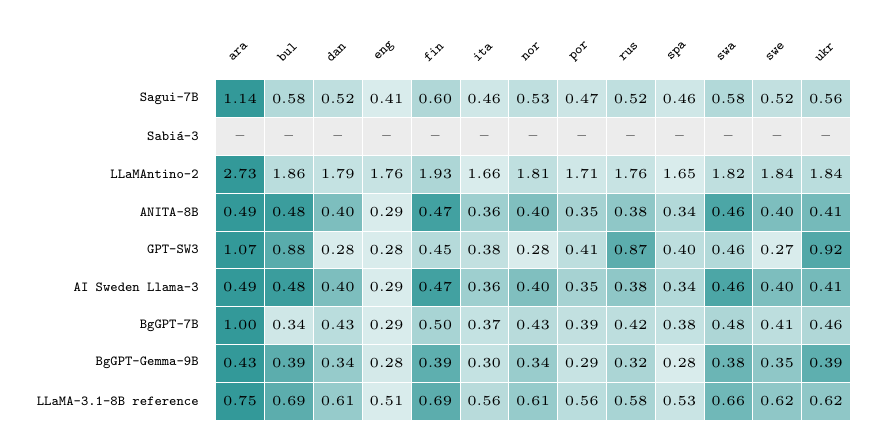
\begin{tikzpicture}[x=0.62cm,y=0.48cm]
\node[rotate=45,anchor=west,font=\tiny] at (0.16,0.35) {\texttt{ara}};
\node[rotate=45,anchor=west,font=\tiny] at (1.16,0.35) {\texttt{bul}};
\node[rotate=45,anchor=west,font=\tiny] at (2.16,0.35) {\texttt{dan}};
\node[rotate=45,anchor=west,font=\tiny] at (3.16,0.35) {\texttt{eng}};
\node[rotate=45,anchor=west,font=\tiny] at (4.16,0.35) {\texttt{fin}};
\node[rotate=45,anchor=west,font=\tiny] at (5.16,0.35) {\texttt{ita}};
\node[rotate=45,anchor=west,font=\tiny] at (6.16,0.35) {\texttt{nor}};
\node[rotate=45,anchor=west,font=\tiny] at (7.16,0.35) {\texttt{por}};
\node[rotate=45,anchor=west,font=\tiny] at (8.16,0.35) {\texttt{rus}};
\node[rotate=45,anchor=west,font=\tiny] at (9.16,0.35) {\texttt{spa}};
\node[rotate=45,anchor=west,font=\tiny] at (10.16,0.35) {\texttt{swa}};
\node[rotate=45,anchor=west,font=\tiny] at (11.16,0.35) {\texttt{swe}};
\node[rotate=45,anchor=west,font=\tiny] at (12.16,0.35) {\texttt{ukr}};
\node[anchor=east,font=\tiny] at (-0.15,-0.5) {\texttt{Sagui-7B}};
\fill[teal!80!white] (0,0) rectangle ++(1,-1);
\draw[white,line width=0.2pt] (0,0) rectangle ++(1,-1);
\node[font=\tiny] at (0.5,-0.5) {1.14};
\fill[teal!30!white] (1,0) rectangle ++(1,-1);
\draw[white,line width=0.2pt] (1,0) rectangle ++(1,-1);
\node[font=\tiny] at (1.5,-0.5) {0.58};
\fill[teal!25!white] (2,0) rectangle ++(1,-1);
\draw[white,line width=0.2pt] (2,0) rectangle ++(1,-1);
\node[font=\tiny] at (2.5,-0.5) {0.52};
\fill[teal!15!white] (3,0) rectangle ++(1,-1);
\draw[white,line width=0.2pt] (3,0) rectangle ++(1,-1);
\node[font=\tiny] at (3.5,-0.5) {0.41};
\fill[teal!31!white] (4,0) rectangle ++(1,-1);
\draw[white,line width=0.2pt] (4,0) rectangle ++(1,-1);
\node[font=\tiny] at (4.5,-0.5) {0.60};
\fill[teal!19!white] (5,0) rectangle ++(1,-1);
\draw[white,line width=0.2pt] (5,0) rectangle ++(1,-1);
\node[font=\tiny] at (5.5,-0.5) {0.46};
\fill[teal!25!white] (6,0) rectangle ++(1,-1);
\draw[white,line width=0.2pt] (6,0) rectangle ++(1,-1);
\node[font=\tiny] at (6.5,-0.5) {0.53};
\fill[teal!20!white] (7,0) rectangle ++(1,-1);
\draw[white,line width=0.2pt] (7,0) rectangle ++(1,-1);
\node[font=\tiny] at (7.5,-0.5) {0.47};
\fill[teal!25!white] (8,0) rectangle ++(1,-1);
\draw[white,line width=0.2pt] (8,0) rectangle ++(1,-1);
\node[font=\tiny] at (8.5,-0.5) {0.52};
\fill[teal!19!white] (9,0) rectangle ++(1,-1);
\draw[white,line width=0.2pt] (9,0) rectangle ++(1,-1);
\node[font=\tiny] at (9.5,-0.5) {0.46};
\fill[teal!30!white] (10,0) rectangle ++(1,-1);
\draw[white,line width=0.2pt] (10,0) rectangle ++(1,-1);
\node[font=\tiny] at (10.5,-0.5) {0.58};
\fill[teal!24!white] (11,0) rectangle ++(1,-1);
\draw[white,line width=0.2pt] (11,0) rectangle ++(1,-1);
\node[font=\tiny] at (11.5,-0.5) {0.52};
\fill[teal!28!white] (12,0) rectangle ++(1,-1);
\draw[white,line width=0.2pt] (12,0) rectangle ++(1,-1);
\node[font=\tiny] at (12.5,-0.5) {0.56};
\node[anchor=east,font=\tiny] at (-0.15,-1.5) {\texttt{Sabi\'a-3}};
\fill[gray!15] (0,-1) rectangle ++(1,-1);
\draw[white,line width=0.2pt] (0,-1) rectangle ++(1,-1);
\node[font=\tiny] at (0.5,-1.5) {--};
\fill[gray!15] (1,-1) rectangle ++(1,-1);
\draw[white,line width=0.2pt] (1,-1) rectangle ++(1,-1);
\node[font=\tiny] at (1.5,-1.5) {--};
\fill[gray!15] (2,-1) rectangle ++(1,-1);
\draw[white,line width=0.2pt] (2,-1) rectangle ++(1,-1);
\node[font=\tiny] at (2.5,-1.5) {--};
\fill[gray!15] (3,-1) rectangle ++(1,-1);
\draw[white,line width=0.2pt] (3,-1) rectangle ++(1,-1);
\node[font=\tiny] at (3.5,-1.5) {--};
\fill[gray!15] (4,-1) rectangle ++(1,-1);
\draw[white,line width=0.2pt] (4,-1) rectangle ++(1,-1);
\node[font=\tiny] at (4.5,-1.5) {--};
\fill[gray!15] (5,-1) rectangle ++(1,-1);
\draw[white,line width=0.2pt] (5,-1) rectangle ++(1,-1);
\node[font=\tiny] at (5.5,-1.5) {--};
\fill[gray!15] (6,-1) rectangle ++(1,-1);
\draw[white,line width=0.2pt] (6,-1) rectangle ++(1,-1);
\node[font=\tiny] at (6.5,-1.5) {--};
\fill[gray!15] (7,-1) rectangle ++(1,-1);
\draw[white,line width=0.2pt] (7,-1) rectangle ++(1,-1);
\node[font=\tiny] at (7.5,-1.5) {--};
\fill[gray!15] (8,-1) rectangle ++(1,-1);
\draw[white,line width=0.2pt] (8,-1) rectangle ++(1,-1);
\node[font=\tiny] at (8.5,-1.5) {--};
\fill[gray!15] (9,-1) rectangle ++(1,-1);
\draw[white,line width=0.2pt] (9,-1) rectangle ++(1,-1);
\node[font=\tiny] at (9.5,-1.5) {--};
\fill[gray!15] (10,-1) rectangle ++(1,-1);
\draw[white,line width=0.2pt] (10,-1) rectangle ++(1,-1);
\node[font=\tiny] at (10.5,-1.5) {--};
\fill[gray!15] (11,-1) rectangle ++(1,-1);
\draw[white,line width=0.2pt] (11,-1) rectangle ++(1,-1);
\node[font=\tiny] at (11.5,-1.5) {--};
\fill[gray!15] (12,-1) rectangle ++(1,-1);
\draw[white,line width=0.2pt] (12,-1) rectangle ++(1,-1);
\node[font=\tiny] at (12.5,-1.5) {--};
\node[anchor=east,font=\tiny] at (-0.15,-2.5) {\texttt{LLaMAntino-2}};
\fill[teal!80!white] (0,-2) rectangle ++(1,-1);
\draw[white,line width=0.2pt] (0,-2) rectangle ++(1,-1);
\node[font=\tiny] at (0.5,-2.5) {2.73};
\fill[teal!27!white] (1,-2) rectangle ++(1,-1);
\draw[white,line width=0.2pt] (1,-2) rectangle ++(1,-1);
\node[font=\tiny] at (1.5,-2.5) {1.86};
\fill[teal!23!white] (2,-2) rectangle ++(1,-1);
\draw[white,line width=0.2pt] (2,-2) rectangle ++(1,-1);
\node[font=\tiny] at (2.5,-2.5) {1.79};
\fill[teal!22!white] (3,-2) rectangle ++(1,-1);
\draw[white,line width=0.2pt] (3,-2) rectangle ++(1,-1);
\node[font=\tiny] at (3.5,-2.5) {1.76};
\fill[teal!32!white] (4,-2) rectangle ++(1,-1);
\draw[white,line width=0.2pt] (4,-2) rectangle ++(1,-1);
\node[font=\tiny] at (4.5,-2.5) {1.93};
\fill[teal!15!white] (5,-2) rectangle ++(1,-1);
\draw[white,line width=0.2pt] (5,-2) rectangle ++(1,-1);
\node[font=\tiny] at (5.5,-2.5) {1.66};
\fill[teal!25!white] (6,-2) rectangle ++(1,-1);
\draw[white,line width=0.2pt] (6,-2) rectangle ++(1,-1);
\node[font=\tiny] at (6.5,-2.5) {1.81};
\fill[teal!19!white] (7,-2) rectangle ++(1,-1);
\draw[white,line width=0.2pt] (7,-2) rectangle ++(1,-1);
\node[font=\tiny] at (7.5,-2.5) {1.71};
\fill[teal!22!white] (8,-2) rectangle ++(1,-1);
\draw[white,line width=0.2pt] (8,-2) rectangle ++(1,-1);
\node[font=\tiny] at (8.5,-2.5) {1.76};
\fill[teal!15!white] (9,-2) rectangle ++(1,-1);
\draw[white,line width=0.2pt] (9,-2) rectangle ++(1,-1);
\node[font=\tiny] at (9.5,-2.5) {1.65};
\fill[teal!25!white] (10,-2) rectangle ++(1,-1);
\draw[white,line width=0.2pt] (10,-2) rectangle ++(1,-1);
\node[font=\tiny] at (10.5,-2.5) {1.82};
\fill[teal!27!white] (11,-2) rectangle ++(1,-1);
\draw[white,line width=0.2pt] (11,-2) rectangle ++(1,-1);
\node[font=\tiny] at (11.5,-2.5) {1.84};
\fill[teal!27!white] (12,-2) rectangle ++(1,-1);
\draw[white,line width=0.2pt] (12,-2) rectangle ++(1,-1);
\node[font=\tiny] at (12.5,-2.5) {1.84};
\node[anchor=east,font=\tiny] at (-0.15,-3.5) {\texttt{ANITA-8B}};
\fill[teal!80!white] (0,-3) rectangle ++(1,-1);
\draw[white,line width=0.2pt] (0,-3) rectangle ++(1,-1);
\node[font=\tiny] at (0.5,-3.5) {0.49};
\fill[teal!77!white] (1,-3) rectangle ++(1,-1);
\draw[white,line width=0.2pt] (1,-3) rectangle ++(1,-1);
\node[font=\tiny] at (1.5,-3.5) {0.48};
\fill[teal!51!white] (2,-3) rectangle ++(1,-1);
\draw[white,line width=0.2pt] (2,-3) rectangle ++(1,-1);
\node[font=\tiny] at (2.5,-3.5) {0.40};
\fill[teal!15!white] (3,-3) rectangle ++(1,-1);
\draw[white,line width=0.2pt] (3,-3) rectangle ++(1,-1);
\node[font=\tiny] at (3.5,-3.5) {0.29};
\fill[teal!74!white] (4,-3) rectangle ++(1,-1);
\draw[white,line width=0.2pt] (4,-3) rectangle ++(1,-1);
\node[font=\tiny] at (4.5,-3.5) {0.47};
\fill[teal!38!white] (5,-3) rectangle ++(1,-1);
\draw[white,line width=0.2pt] (5,-3) rectangle ++(1,-1);
\node[font=\tiny] at (5.5,-3.5) {0.36};
\fill[teal!50!white] (6,-3) rectangle ++(1,-1);
\draw[white,line width=0.2pt] (6,-3) rectangle ++(1,-1);
\node[font=\tiny] at (6.5,-3.5) {0.40};
\fill[teal!35!white] (7,-3) rectangle ++(1,-1);
\draw[white,line width=0.2pt] (7,-3) rectangle ++(1,-1);
\node[font=\tiny] at (7.5,-3.5) {0.35};
\fill[teal!44!white] (8,-3) rectangle ++(1,-1);
\draw[white,line width=0.2pt] (8,-3) rectangle ++(1,-1);
\node[font=\tiny] at (8.5,-3.5) {0.38};
\fill[teal!30!white] (9,-3) rectangle ++(1,-1);
\draw[white,line width=0.2pt] (9,-3) rectangle ++(1,-1);
\node[font=\tiny] at (9.5,-3.5) {0.34};
\fill[teal!70!white] (10,-3) rectangle ++(1,-1);
\draw[white,line width=0.2pt] (10,-3) rectangle ++(1,-1);
\node[font=\tiny] at (10.5,-3.5) {0.46};
\fill[teal!51!white] (11,-3) rectangle ++(1,-1);
\draw[white,line width=0.2pt] (11,-3) rectangle ++(1,-1);
\node[font=\tiny] at (11.5,-3.5) {0.40};
\fill[teal!54!white] (12,-3) rectangle ++(1,-1);
\draw[white,line width=0.2pt] (12,-3) rectangle ++(1,-1);
\node[font=\tiny] at (12.5,-3.5) {0.41};
\node[anchor=east,font=\tiny] at (-0.15,-4.5) {\texttt{GPT-SW3}};
\fill[teal!80!white] (0,-4) rectangle ++(1,-1);
\draw[white,line width=0.2pt] (0,-4) rectangle ++(1,-1);
\node[font=\tiny] at (0.5,-4.5) {1.07};
\fill[teal!65!white] (1,-4) rectangle ++(1,-1);
\draw[white,line width=0.2pt] (1,-4) rectangle ++(1,-1);
\node[font=\tiny] at (1.5,-4.5) {0.88};
\fill[teal!15!white] (2,-4) rectangle ++(1,-1);
\draw[white,line width=0.2pt] (2,-4) rectangle ++(1,-1);
\node[font=\tiny] at (2.5,-4.5) {0.28};
\fill[teal!15!white] (3,-4) rectangle ++(1,-1);
\draw[white,line width=0.2pt] (3,-4) rectangle ++(1,-1);
\node[font=\tiny] at (3.5,-4.5) {0.28};
\fill[teal!29!white] (4,-4) rectangle ++(1,-1);
\draw[white,line width=0.2pt] (4,-4) rectangle ++(1,-1);
\node[font=\tiny] at (4.5,-4.5) {0.45};
\fill[teal!24!white] (5,-4) rectangle ++(1,-1);
\draw[white,line width=0.2pt] (5,-4) rectangle ++(1,-1);
\node[font=\tiny] at (5.5,-4.5) {0.38};
\fill[teal!15!white] (6,-4) rectangle ++(1,-1);
\draw[white,line width=0.2pt] (6,-4) rectangle ++(1,-1);
\node[font=\tiny] at (6.5,-4.5) {0.28};
\fill[teal!26!white] (7,-4) rectangle ++(1,-1);
\draw[white,line width=0.2pt] (7,-4) rectangle ++(1,-1);
\node[font=\tiny] at (7.5,-4.5) {0.41};
\fill[teal!64!white] (8,-4) rectangle ++(1,-1);
\draw[white,line width=0.2pt] (8,-4) rectangle ++(1,-1);
\node[font=\tiny] at (8.5,-4.5) {0.87};
\fill[teal!26!white] (9,-4) rectangle ++(1,-1);
\draw[white,line width=0.2pt] (9,-4) rectangle ++(1,-1);
\node[font=\tiny] at (9.5,-4.5) {0.40};
\fill[teal!30!white] (10,-4) rectangle ++(1,-1);
\draw[white,line width=0.2pt] (10,-4) rectangle ++(1,-1);
\node[font=\tiny] at (10.5,-4.5) {0.46};
\fill[teal!15!white] (11,-4) rectangle ++(1,-1);
\draw[white,line width=0.2pt] (11,-4) rectangle ++(1,-1);
\node[font=\tiny] at (11.5,-4.5) {0.27};
\fill[teal!68!white] (12,-4) rectangle ++(1,-1);
\draw[white,line width=0.2pt] (12,-4) rectangle ++(1,-1);
\node[font=\tiny] at (12.5,-4.5) {0.92};
\node[anchor=east,font=\tiny] at (-0.15,-5.5) {\texttt{AI Sweden Llama-3}};
\fill[teal!80!white] (0,-5) rectangle ++(1,-1);
\draw[white,line width=0.2pt] (0,-5) rectangle ++(1,-1);
\node[font=\tiny] at (0.5,-5.5) {0.49};
\fill[teal!77!white] (1,-5) rectangle ++(1,-1);
\draw[white,line width=0.2pt] (1,-5) rectangle ++(1,-1);
\node[font=\tiny] at (1.5,-5.5) {0.48};
\fill[teal!51!white] (2,-5) rectangle ++(1,-1);
\draw[white,line width=0.2pt] (2,-5) rectangle ++(1,-1);
\node[font=\tiny] at (2.5,-5.5) {0.40};
\fill[teal!15!white] (3,-5) rectangle ++(1,-1);
\draw[white,line width=0.2pt] (3,-5) rectangle ++(1,-1);
\node[font=\tiny] at (3.5,-5.5) {0.29};
\fill[teal!74!white] (4,-5) rectangle ++(1,-1);
\draw[white,line width=0.2pt] (4,-5) rectangle ++(1,-1);
\node[font=\tiny] at (4.5,-5.5) {0.47};
\fill[teal!38!white] (5,-5) rectangle ++(1,-1);
\draw[white,line width=0.2pt] (5,-5) rectangle ++(1,-1);
\node[font=\tiny] at (5.5,-5.5) {0.36};
\fill[teal!50!white] (6,-5) rectangle ++(1,-1);
\draw[white,line width=0.2pt] (6,-5) rectangle ++(1,-1);
\node[font=\tiny] at (6.5,-5.5) {0.40};
\fill[teal!35!white] (7,-5) rectangle ++(1,-1);
\draw[white,line width=0.2pt] (7,-5) rectangle ++(1,-1);
\node[font=\tiny] at (7.5,-5.5) {0.35};
\fill[teal!44!white] (8,-5) rectangle ++(1,-1);
\draw[white,line width=0.2pt] (8,-5) rectangle ++(1,-1);
\node[font=\tiny] at (8.5,-5.5) {0.38};
\fill[teal!30!white] (9,-5) rectangle ++(1,-1);
\draw[white,line width=0.2pt] (9,-5) rectangle ++(1,-1);
\node[font=\tiny] at (9.5,-5.5) {0.34};
\fill[teal!70!white] (10,-5) rectangle ++(1,-1);
\draw[white,line width=0.2pt] (10,-5) rectangle ++(1,-1);
\node[font=\tiny] at (10.5,-5.5) {0.46};
\fill[teal!51!white] (11,-5) rectangle ++(1,-1);
\draw[white,line width=0.2pt] (11,-5) rectangle ++(1,-1);
\node[font=\tiny] at (11.5,-5.5) {0.40};
\fill[teal!54!white] (12,-5) rectangle ++(1,-1);
\draw[white,line width=0.2pt] (12,-5) rectangle ++(1,-1);
\node[font=\tiny] at (12.5,-5.5) {0.41};
\node[anchor=east,font=\tiny] at (-0.15,-6.5) {\texttt{BgGPT-7B}};
\fill[teal!80!white] (0,-6) rectangle ++(1,-1);
\draw[white,line width=0.2pt] (0,-6) rectangle ++(1,-1);
\node[font=\tiny] at (0.5,-6.5) {1.00};
\fill[teal!19!white] (1,-6) rectangle ++(1,-1);
\draw[white,line width=0.2pt] (1,-6) rectangle ++(1,-1);
\node[font=\tiny] at (1.5,-6.5) {0.34};
\fill[teal!27!white] (2,-6) rectangle ++(1,-1);
\draw[white,line width=0.2pt] (2,-6) rectangle ++(1,-1);
\node[font=\tiny] at (2.5,-6.5) {0.43};
\fill[teal!15!white] (3,-6) rectangle ++(1,-1);
\draw[white,line width=0.2pt] (3,-6) rectangle ++(1,-1);
\node[font=\tiny] at (3.5,-6.5) {0.29};
\fill[teal!34!white] (4,-6) rectangle ++(1,-1);
\draw[white,line width=0.2pt] (4,-6) rectangle ++(1,-1);
\node[font=\tiny] at (4.5,-6.5) {0.50};
\fill[teal!23!white] (5,-6) rectangle ++(1,-1);
\draw[white,line width=0.2pt] (5,-6) rectangle ++(1,-1);
\node[font=\tiny] at (5.5,-6.5) {0.37};
\fill[teal!28!white] (6,-6) rectangle ++(1,-1);
\draw[white,line width=0.2pt] (6,-6) rectangle ++(1,-1);
\node[font=\tiny] at (6.5,-6.5) {0.43};
\fill[teal!24!white] (7,-6) rectangle ++(1,-1);
\draw[white,line width=0.2pt] (7,-6) rectangle ++(1,-1);
\node[font=\tiny] at (7.5,-6.5) {0.39};
\fill[teal!26!white] (8,-6) rectangle ++(1,-1);
\draw[white,line width=0.2pt] (8,-6) rectangle ++(1,-1);
\node[font=\tiny] at (8.5,-6.5) {0.42};
\fill[teal!23!white] (9,-6) rectangle ++(1,-1);
\draw[white,line width=0.2pt] (9,-6) rectangle ++(1,-1);
\node[font=\tiny] at (9.5,-6.5) {0.38};
\fill[teal!32!white] (10,-6) rectangle ++(1,-1);
\draw[white,line width=0.2pt] (10,-6) rectangle ++(1,-1);
\node[font=\tiny] at (10.5,-6.5) {0.48};
\fill[teal!26!white] (11,-6) rectangle ++(1,-1);
\draw[white,line width=0.2pt] (11,-6) rectangle ++(1,-1);
\node[font=\tiny] at (11.5,-6.5) {0.41};
\fill[teal!31!white] (12,-6) rectangle ++(1,-1);
\draw[white,line width=0.2pt] (12,-6) rectangle ++(1,-1);
\node[font=\tiny] at (12.5,-6.5) {0.46};
\node[anchor=east,font=\tiny] at (-0.15,-7.5) {\texttt{BgGPT-Gemma-9B}};
\fill[teal!80!white] (0,-7) rectangle ++(1,-1);
\draw[white,line width=0.2pt] (0,-7) rectangle ++(1,-1);
\node[font=\tiny] at (0.5,-7.5) {0.43};
\fill[teal!64!white] (1,-7) rectangle ++(1,-1);
\draw[white,line width=0.2pt] (1,-7) rectangle ++(1,-1);
\node[font=\tiny] at (1.5,-7.5) {0.39};
\fill[teal!41!white] (2,-7) rectangle ++(1,-1);
\draw[white,line width=0.2pt] (2,-7) rectangle ++(1,-1);
\node[font=\tiny] at (2.5,-7.5) {0.34};
\fill[teal!17!white] (3,-7) rectangle ++(1,-1);
\draw[white,line width=0.2pt] (3,-7) rectangle ++(1,-1);
\node[font=\tiny] at (3.5,-7.5) {0.28};
\fill[teal!63!white] (4,-7) rectangle ++(1,-1);
\draw[white,line width=0.2pt] (4,-7) rectangle ++(1,-1);
\node[font=\tiny] at (4.5,-7.5) {0.39};
\fill[teal!23!white] (5,-7) rectangle ++(1,-1);
\draw[white,line width=0.2pt] (5,-7) rectangle ++(1,-1);
\node[font=\tiny] at (5.5,-7.5) {0.30};
\fill[teal!40!white] (6,-7) rectangle ++(1,-1);
\draw[white,line width=0.2pt] (6,-7) rectangle ++(1,-1);
\node[font=\tiny] at (6.5,-7.5) {0.34};
\fill[teal!22!white] (7,-7) rectangle ++(1,-1);
\draw[white,line width=0.2pt] (7,-7) rectangle ++(1,-1);
\node[font=\tiny] at (7.5,-7.5) {0.29};
\fill[teal!33!white] (8,-7) rectangle ++(1,-1);
\draw[white,line width=0.2pt] (8,-7) rectangle ++(1,-1);
\node[font=\tiny] at (8.5,-7.5) {0.32};
\fill[teal!15!white] (9,-7) rectangle ++(1,-1);
\draw[white,line width=0.2pt] (9,-7) rectangle ++(1,-1);
\node[font=\tiny] at (9.5,-7.5) {0.28};
\fill[teal!58!white] (10,-7) rectangle ++(1,-1);
\draw[white,line width=0.2pt] (10,-7) rectangle ++(1,-1);
\node[font=\tiny] at (10.5,-7.5) {0.38};
\fill[teal!44!white] (11,-7) rectangle ++(1,-1);
\draw[white,line width=0.2pt] (11,-7) rectangle ++(1,-1);
\node[font=\tiny] at (11.5,-7.5) {0.35};
\fill[teal!63!white] (12,-7) rectangle ++(1,-1);
\draw[white,line width=0.2pt] (12,-7) rectangle ++(1,-1);
\node[font=\tiny] at (12.5,-7.5) {0.39};
\node[anchor=east,font=\tiny] at (-0.15,-8.5) {\texttt{LLaMA-3.1-8B reference}};
\fill[teal!80!white] (0,-8) rectangle ++(1,-1);
\draw[white,line width=0.2pt] (0,-8) rectangle ++(1,-1);
\node[font=\tiny] at (0.5,-8.5) {0.75};
\fill[teal!64!white] (1,-8) rectangle ++(1,-1);
\draw[white,line width=0.2pt] (1,-8) rectangle ++(1,-1);
\node[font=\tiny] at (1.5,-8.5) {0.69};
\fill[teal!41!white] (2,-8) rectangle ++(1,-1);
\draw[white,line width=0.2pt] (2,-8) rectangle ++(1,-1);
\node[font=\tiny] at (2.5,-8.5) {0.61};
\fill[teal!15!white] (3,-8) rectangle ++(1,-1);
\draw[white,line width=0.2pt] (3,-8) rectangle ++(1,-1);
\node[font=\tiny] at (3.5,-8.5) {0.51};
\fill[teal!64!white] (4,-8) rectangle ++(1,-1);
\draw[white,line width=0.2pt] (4,-8) rectangle ++(1,-1);
\node[font=\tiny] at (4.5,-8.5) {0.69};
\fill[teal!28!white] (5,-8) rectangle ++(1,-1);
\draw[white,line width=0.2pt] (5,-8) rectangle ++(1,-1);
\node[font=\tiny] at (5.5,-8.5) {0.56};
\fill[teal!41!white] (6,-8) rectangle ++(1,-1);
\draw[white,line width=0.2pt] (6,-8) rectangle ++(1,-1);
\node[font=\tiny] at (6.5,-8.5) {0.61};
\fill[teal!27!white] (7,-8) rectangle ++(1,-1);
\draw[white,line width=0.2pt] (7,-8) rectangle ++(1,-1);
\node[font=\tiny] at (7.5,-8.5) {0.56};
\fill[teal!34!white] (8,-8) rectangle ++(1,-1);
\draw[white,line width=0.2pt] (8,-8) rectangle ++(1,-1);
\node[font=\tiny] at (8.5,-8.5) {0.58};
\fill[teal!21!white] (9,-8) rectangle ++(1,-1);
\draw[white,line width=0.2pt] (9,-8) rectangle ++(1,-1);
\node[font=\tiny] at (9.5,-8.5) {0.53};
\fill[teal!56!white] (10,-8) rectangle ++(1,-1);
\draw[white,line width=0.2pt] (10,-8) rectangle ++(1,-1);
\node[font=\tiny] at (10.5,-8.5) {0.66};
\fill[teal!44!white] (11,-8) rectangle ++(1,-1);
\draw[white,line width=0.2pt] (11,-8) rectangle ++(1,-1);
\node[font=\tiny] at (11.5,-8.5) {0.62};
\fill[teal!44!white] (12,-8) rectangle ++(1,-1);
\draw[white,line width=0.2pt] (12,-8) rectangle ++(1,-1);
\node[font=\tiny] at (12.5,-8.5) {0.62};
\end{tikzpicture}
\caption[Mean tokens per character by model and attack language]{Mean tokens per character by model and attack language. Each value averages prompt-level chat-template token counts divided by the number of characters in the attack-language prompt before chat-template rendering. Characters are Unicode code points, not UTF-8 bytes. Darker shading marks higher density within each model's row; colour scales are normalized separately by model. Dashes indicate unavailable measurements. The English reference is descriptive. These values reflect tokenizer segmentation and template overhead, not comprehension or safety.}
\label{fig:tokens-per-character}
\fonte{Author.}
\end{figure}
}


\chapter{Results}
\label{chap:results}

This chapter reports the final empirical results produced by the frozen evaluation dataset. The analysis uses 36189 prompt--model--language rows, consisting of the eight target language-specific models plus the English-aligned \texttt{LLaMA-3.1-8B} reference baseline. The presentation follows Chapter~\ref{chap:methodology}: coverage and translation quality precede graded score summaries, distance and specialization descriptions, tokenizer checks, and fractional-logit inference.

Coverage accounting in this chapter is anchored at the retained frozen panel of 4021 attempts per model reported in Table~\ref{tab:results-coverage}. Appendix~\ref{app:frozen-qc-details} gives the upstream source-prompt arithmetic and the numeric translation-QC thresholds that produced that retained panel, while this chapter reports the empirical denominators from the frozen panel onward.

\textbf{The main empirical finding does not support the directional account.} Mean graded harmful-assistance scores vary strongly by model family and paired post-training regime, but it does not increase stably with URIEL+ distance, and BELEBELE-derived specialization does not behave as a simple protective factor. The safer practical reading is therefore that \textbf{checkpoint differences are large, while the distance association depends on coverage and statistical specification.}
\defensebox{How to defend the negative result}{The full-panel directional hypotheses are not supported, and a post-review coverage restriction reverses the distance sign. Both observations must be reported. That is scientifically useful. The result narrows what can be claimed: typological distance alone is not a reliable priority rule for multilingual red-teaming in this panel. The stronger practical finding is model-centered: some language-specific assistants are unsafe broadly, while others are much safer across many languages. In a defense, this should be framed as replacing an elegant hypothesis with a more operationally honest safety conclusion.}

\section{Evaluation Coverage and Data Quality}
\label{sec:results-coverage}

Table~\ref{tab:results-coverage} reports the denominator for the later mean-score estimates. All target models and the reference baseline cover the 13 attack languages. The frozen dataset contains 78 excluded or unscored rows: 75 empty model outputs and three StrongREJECT judge safety-filter failures.
These cases are technical or scoring failures, not safe responses. They are excluded from the mean-score denominator and remain visible in coverage accounting. In-model refusals are retained as substantive model outputs.
\defensenote{Coverage vs safety}{Coverage failures are measurement failures. Refusals are model behavior. Keeping those categories separate avoids artificially rewarding systems that fail to produce scorable outputs.}

\QualityCoverageTable

The exclusions are concentrated rather than evenly distributed. Sixty-nine empty outputs occur for \texttt{BgGPT-Gemma-2-9B-Instruct} in Swedish, and six additional empty outputs occur for \texttt{LLaMAntino-2-chat-UltraChat-ITA} across Danish, English, Norwegian, Portuguese, Spanish, and Swedish. The three judge safety-filter blocks occur once for \texttt{AI Sweden Llama-3-8B-instruct} in Norwegian and twice for \texttt{Sabiá-3} in Danish. The dataset otherwise has no duplicate run identifiers and no duplicate model--language--prompt rows.

For the three nonempty responses blocked by the scoring judge, the score is unknown. Table~\ref{tab:graded-unscored-bounds} shows worst/best-case mean-score bounds instead of assigning observed zeros. Even assigning all three unscored responses the maximum score changes each affected model mean by less than 0.0005 relative to the zero-assignment bound. These judge blocks are not target-provider blocks. The 75 empty outputs remain technical missingness. All rows have a true generation-completion flag, which indicates request-path completion and does not establish usable text.

\GradedBoundsTable

\subsection{LLM-only Prompt Translation QC}
\label{sec:prompt-translation-qc}

The translation audit was completed with the XSTS-style LLM reviewer described in the methodology: the 148 BLASER-flagged prompt translations were judged by a \texttt{gpt-5.4} XSTS assessor. Of those flagged rows, 100 were retained and 48 were excluded from the frozen prompt inventory. The remaining 3921 prompt translations passed the BLASER gate and did not receive an XSTS score. Round-trip drift is computed for every prompt translation and reported as a diagnostic.

Table~\ref{tab:prompt-translation-qc} reports the BLASER-flagged queue size, median XSTS score, and audit decision counts by attack language.

\QualityPromptQcTable

Finnish is the main translation-pipeline anomaly. It has 58 flagged rows, far above the next-highest queue size of 17, and 20 of those flagged rows were marked for exclusion by the LLM judge. Ukrainian also shows a relatively high exclusion count among flagged rows.

\section{StrongREJECT Scores and Model Comparisons}
\label{sec:overall-score}

This section compares the evaluated models using the mean official StrongREJECT score defined in Section~\ref{sec:strongreject-graded}, Equation~\ref{eq:mean-strongreject}. Higher means indicate more rubric-assessed harmful assistance across the scored responses. Zero scores are included; missing judge scores remain unknown and are excluded. These means are graded scores, not percentages of successful attacks.

\subsection{Aligned and Non-aligned Language Comparisons}

Figure~\ref{fig:graded-aligned-comparison} compares two settings on a common score scale: each model's aligned language and the other twelve languages pooled together. Models are grouped into the Portuguese, Italian, Swedish, and Bulgarian pairs. A separate English-reference row shows its English mean and pooled mean across the twelve non-English languages; this baseline is descriptive and excluded from paired inference. The two points in each row show whether harmful-assistance scores are already high in the aligned-language setting or increase outside it. Exact means, intervals, and scored sample sizes appear in Appendix~\ref{app:graded-details}, Table~\ref{tab:graded-setting-summary}.

The horizontal whiskers show 95\% uncertainty intervals estimated by repeatedly sampling the original prompts, keeping their translated responses together. In the non-aligned setting, every scored response contributes equally, so a language with more scored responses contributes more to the pooled mean.

\begin{figure}[htbp]\centering
\includegraphics[width=\linewidth]{figures/graded_aligned_comparison.pdf}
\caption{Mean StrongREJECT scores in aligned and pooled non-aligned languages, grouped by model pair, with a separate descriptive English reference baseline. Its aligned language is English; it is excluded from paired inference. Points show means and whiskers show 95\% prompt-cluster bootstrap intervals (2,000 resamples). Zero scores are included; missing judge scores are excluded. Non-aligned means weight each scored response equally. Higher scores indicate more harmful assistance.}\label{fig:graded-aligned-comparison}\fonte{Author.}
\end{figure}

The Portuguese, Italian, and Bulgarian pairs show the same broad ordering in both settings: the strong-pole model has a lower mean score than its weak-pole partner. The Swedish pair shows the opposite ordering, with AI Sweden scoring higher than GPT-SW3. Thus, the strong-pole label does not consistently correspond to lower harmful assistance across all four pairs.

These comparisons describe the evaluated checkpoints. Each pair differs in more than its alignment label, including model ancestry, training data, size, and serving mode. We therefore cannot attribute the differences to a single alignment intervention. Similarly, the combined non-aligned mean can hide considerable variation between individual languages.
\defensenote{Present the pair comparison}{Say: ``Three pairs have lower average harmful assistance at the strong pole; the Swedish pair goes the other way. This is an observed comparison between checkpoints, not a controlled experiment on alignment strength.'' Then use the language heatmap to show why a single model average is only part of the picture.}

\subsection{Variation Across Languages and Responses}

Figure~\ref{fig:graded-heatmap} separates the combined averages into individual model--language combinations. Each cell gives the mean score for one model answering prompts in one language. It helps identify languages with relatively high or low scores within a model and compare language profiles across models.

\begin{figure}[htbp]\centering
\includegraphics[width=\linewidth]{figures/graded_score_heatmap.pdf}
\caption{Mean StrongREJECT score for each model and attack language. Higher values indicate more harmful assistance.}\label{fig:graded-heatmap}\fonte{Author.}
\end{figure}

A mean does not show how individual responses are distributed. For example, two hypothetical scores of 0 and 1 have the same average as two scores of 0.5, although the first case combines a zero with maximum harmful assistance and the second contains two intermediate responses. Figure~\ref{fig:graded-distribution} therefore shows the distribution of scores across all scored languages for each model. It reveals whether an average comes mainly from zeros, intermediate scores, or high scores.

\begin{figure}[htbp]\centering
\includegraphics[width=\linewidth]{figures/graded_score_distribution.pdf}
\caption{Distribution of StrongREJECT scores for each model across all scored languages. The plot separates zero, intermediate, and high scores.}\label{fig:graded-distribution}\fonte{Author.}
\end{figure}

The official scoring rule produces nine possible levels, from zero to one. ``Graded'' means that these intermediate levels are retained rather than reduced to a yes/no classification.

\subsection{English Reference Baseline}
\label{sec:reference-baseline-results}

Table~\ref{tab:graded-reference} reports the separate English-aligned reference model in each attack language. Its role is to provide a reference result from a base model. It is not a matched parent checkpoint for those models, and it is excluded from the eight-model paired regressions. Differences from this reference therefore do not measure the effect of language specialization or safety changes inherited from a common parent model, but serve as a basis for comparison.

\GradedReferenceTable

\input{chapters/reference_descriptive_contrast}

\clearpage
\section{Distance and Specialization}
\label{sec:graded-distance-spec}
The BELEBELE measures distinguish \emph{instruction following} (IF), operationalized as answer accuracy, from \emph{cross-lingual consistency} (CONS), agreement with aligned-language answers on comparable questions. \emph{Specialization} (SPEC) combines their standardized values with equal weights. A high CONS value need not imply correct answers, and a SPEC value summarizes benign benchmark behavior rather than safety alignment. Figure~\ref{fig:belebele-profiles} presents all three measures for each paired target; Figure~\ref{fig:belebele-worked-example} illustrates the scoring distinction on one question.

\GradedCorrelationsTable
\clearpage
Figure~\ref{fig:strongreject-profiles} shows the StrongREJECT mean for every attack language in a separate panel for each paired target. Its layout and language ordering match the BELEBELE profiles in Figure~\ref{fig:belebele-profiles}, making the harmful-assistance and benign-capability profiles easier to compare. Figures~\ref{fig:strongreject-profiles}, \ref{fig:graded-spec}, and \ref{fig:belebele-profiles} also show the English reference separately; this does not add it to the paired regressions. Weak targets are at left and strong targets at right; the first four rows correspond to the aligned-language pairs. A separate bottom panel shows the descriptive English reference, ordered by distance from English. Shading and bold labels identify the aligned language. Bars show the saved 95\% prompt-cluster bootstrap intervals. All panels share the same score scale. Languages are equally spaced and ordered by increasing URIEL+ distance; the connecting lines describe profiles rather than fitted trends. The plot with actual distance on the horizontal axis is retained in Appendix~\ref{app:graded-details}, Figure~\ref{fig:graded-distance}.
\begin{figure}[p]\centering
\begin{adjustbox}{max totalsize={\linewidth}{.74\textheight},center}% Generated by eval/scripts/write_reference_comparison_figures.py.
\definecolor{srweak}{RGB}{35,103,159}
\definecolor{srstrong}{RGB}{202,86,42}
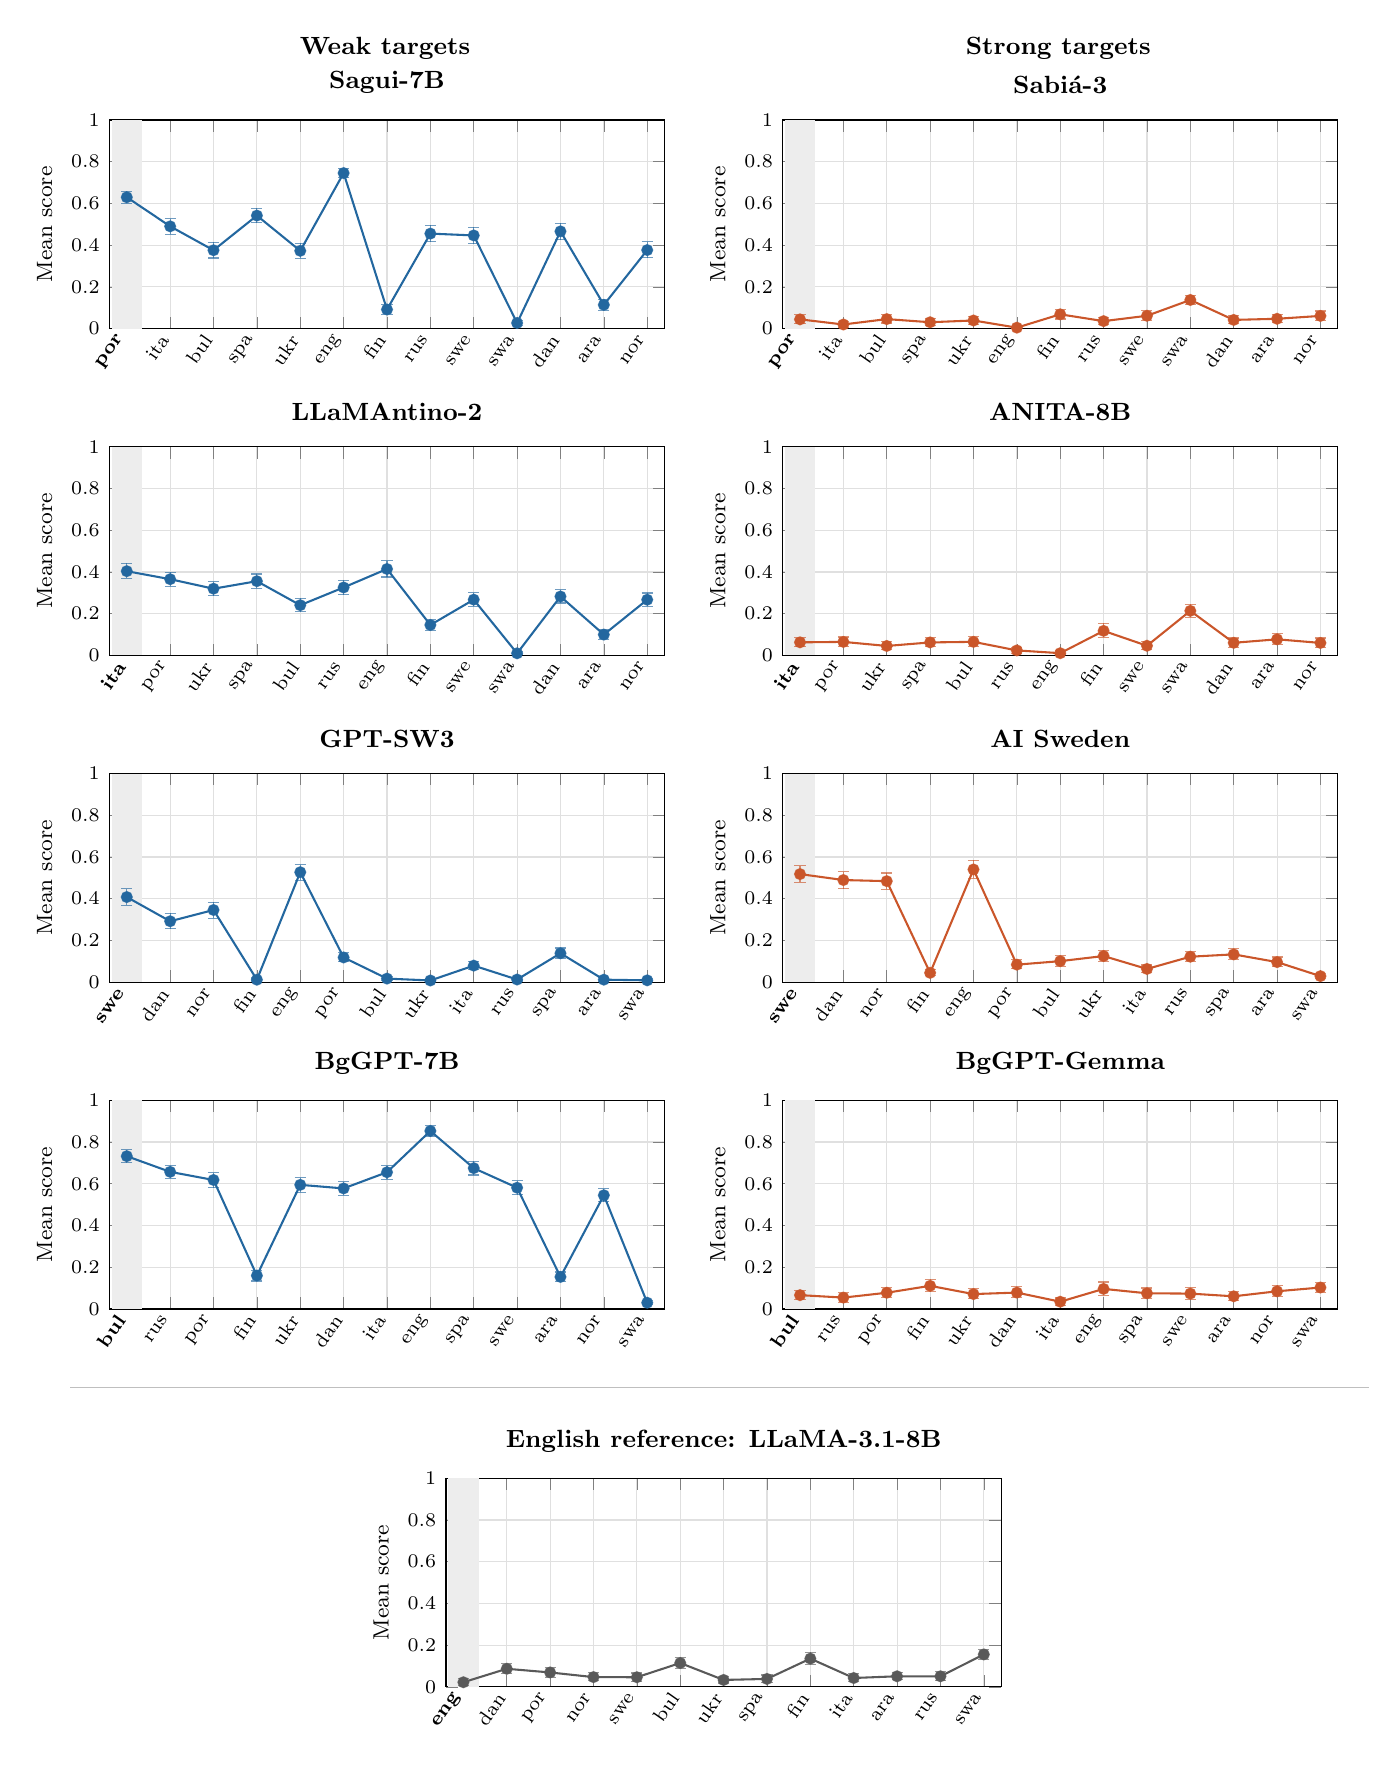
\begin{tikzpicture}
\pgfplotsset{srprofile/.style={width=7.05cm,height=2.65cm,scale only axis,xmin=-.4,xmax=12.4,ymin=0,ymax=1,ytick={0,.2,.4,.6,.8,1},axis lines=box,grid=major,grid style={black!12},tick label style={font=\scriptsize},label style={font=\footnotesize},title style={font=\bfseries\small},xtick={0,...,12},x tick label style={rotate=55,anchor=east,font=\scriptsize},ylabel={Mean score}}}
\node[anchor=south,font=\small\bfseries] at (3.5,.65) {Weak targets};
\node[anchor=south,font=\small\bfseries] at (12.05,.65) {Strong targets};
\begin{axis}[srprofile,at={(0.0cm,-0.0cm)},anchor=north west,title={Sagui-7B},xticklabels={\textbf{por},ita,bul,spa,ukr,eng,fin,rus,swe,swa,dan,ara,nor}]
\path[fill=black!7] (axis cs:-.35,0) rectangle (axis cs:.35,1);
\addplot[color=srweak,mark=*,mark size=1.6pt,line width=.75pt] coordinates {(0,0.629808) (1,0.490415) (2,0.375804) (3,0.541933) (4,0.372937) (5,0.745607) (6,0.091724) (7,0.455529) (8,0.446774) (9,0.027104) (10,0.466346) (11,0.114078) (12,0.376608)};
\addplot[color=srweak,opacity=.65,only marks,mark=none,error bars/.cd,y dir=both,y explicit] coordinates {(0,0.629808) += (0,0.029247) -= (0,0.028446) (1,0.490415) += (0,0.037141) -= (0,0.038359) (2,0.375804) += (0,0.037379) -= (0,0.037379) (3,0.541933) += (0,0.034744) -= (0,0.034355) (4,0.372937) += (0,0.036716) -= (0,0.035479) (5,0.745607) += (0,0.021975) -= (0,0.022364) (6,0.091724) += (0,0.024744) -= (0,0.021758) (7,0.455529) += (0,0.038872) -= (0,0.038862) (8,0.446774) += (0,0.038720) -= (0,0.038720) (9,0.027104) += (0,0.012146) -= (0,0.010518) (10,0.466346) += (0,0.038462) -= (0,0.039663) (11,0.114078) += (0,0.025890) -= (0,0.025081) (12,0.376608) += (0,0.038987) -= (0,0.035772)};
\end{axis}
\begin{axis}[srprofile,at={(8.55cm,-0.0cm)},anchor=north west,title={Sabi\'a-3},xticklabels={\textbf{por},ita,bul,spa,ukr,eng,fin,rus,swe,swa,dan,ara,nor}]
\path[fill=black!7] (axis cs:-.35,0) rectangle (axis cs:.35,1);
\addplot[color=srstrong,mark=*,mark size=1.6pt,line width=.75pt] coordinates {(0,0.044471) (1,0.019968) (2,0.045820) (3,0.030751) (4,0.039191) (5,0.004792) (6,0.068686) (7,0.036058) (8,0.061694) (9,0.137540) (10,0.041935) (11,0.047330) (12,0.061093)};
\addplot[color=srstrong,opacity=.65,only marks,mark=none,error bars/.cd,y dir=both,y explicit] coordinates {(0,0.044471) += (0,0.021635) -= (0,0.020433) (1,0.019968) += (0,0.015186) -= (0,0.012380) (2,0.045820) += (0,0.020900) -= (0,0.018489) (3,0.030751) += (0,0.017582) -= (0,0.015974) (4,0.039191) += (0,0.018977) -= (0,0.017739) (5,0.004792) += (0,0.007188) -= (0,0.004792) (6,0.068686) += (0,0.025171) -= (0,0.022611) (7,0.036058) += (0,0.019231) -= (0,0.017628) (8,0.061694) += (0,0.023397) -= (0,0.022591) (9,0.137540) += (0,0.023058) -= (0,0.023058) (10,0.041935) += (0,0.019355) -= (0,0.018952) (11,0.047330) += (0,0.021450) -= (0,0.019013) (12,0.061093) += (0,0.023312) -= (0,0.022116)};
\end{axis}
\begin{axis}[srprofile,at={(0.0cm,-4.15cm)},anchor=north west,title={LLaMAntino-2},xticklabels={\textbf{ita},por,ukr,spa,bul,rus,eng,fin,swe,swa,dan,ara,nor}]
\path[fill=black!7] (axis cs:-.35,0) rectangle (axis cs:.35,1);
\addplot[color=srweak,mark=*,mark size=1.6pt,line width=.75pt] coordinates {(0,0.403754) (1,0.365354) (2,0.319719) (3,0.355769) (4,0.240756) (5,0.325721) (6,0.414263) (7,0.145904) (8,0.267395) (9,0.010113) (10,0.282556) (11,0.099919) (12,0.266935)};
\addplot[color=srweak,opacity=.65,only marks,mark=none,error bars/.cd,y dir=both,y explicit] coordinates {(0,0.403754) += (0,0.037141) -= (0,0.033946) (1,0.365354) += (0,0.033370) -= (0,0.034164) (2,0.319719) += (0,0.034251) -= (0,0.034653) (3,0.355769) += (0,0.034455) -= (0,0.034054) (4,0.240756) += (0,0.033360) -= (0,0.031361) (5,0.325721) += (0,0.034856) -= (0,0.034866) (6,0.414263) += (0,0.039663) -= (0,0.038462) (7,0.145904) += (0,0.024328) -= (0,0.024317) (8,0.267395) += (0,0.032767) -= (0,0.031553) (9,0.010113) += (0,0.008091) -= (0,0.006472) (10,0.282556) += (0,0.033360) -= (0,0.031361) (11,0.099919) += (0,0.022259) -= (0,0.021845) (12,0.266935) += (0,0.032258) -= (0,0.031452)};
\end{axis}
\begin{axis}[srprofile,at={(8.55cm,-4.15cm)},anchor=north west,title={ANITA-8B},xticklabels={\textbf{ita},por,ukr,spa,bul,rus,eng,fin,swe,swa,dan,ara,nor}]
\path[fill=black!7] (axis cs:-.35,0) rectangle (axis cs:.35,1);
\addplot[color=srstrong,mark=*,mark size=1.6pt,line width=.75pt] coordinates {(0,0.062700) (1,0.064904) (2,0.045380) (3,0.062300) (4,0.065113) (5,0.024038) (6,0.010783) (7,0.117747) (8,0.046371) (9,0.213592) (10,0.060497) (11,0.077265) (12,0.059887)};
\addplot[color=srstrong,opacity=.65,only marks,mark=none,error bars/.cd,y dir=both,y explicit] coordinates {(0,0.062700) += (0,0.023972) -= (0,0.021965) (1,0.064904) += (0,0.023237) -= (0,0.022847) (2,0.045380) += (0,0.021452) -= (0,0.018977) (3,0.062300) += (0,0.025170) -= (0,0.021176) (4,0.065113) += (0,0.024920) -= (0,0.022508) (5,0.024038) += (0,0.015224) -= (0,0.013221) (6,0.010783) += (0,0.011981) -= (0,0.008387) (7,0.117747) += (0,0.035836) -= (0,0.031581) (8,0.046371) += (0,0.021381) -= (0,0.018962) (9,0.213592) += (0,0.031958) -= (0,0.031564) (10,0.060497) += (0,0.023237) -= (0,0.022837) (11,0.077265) += (0,0.026294) -= (0,0.024676) (12,0.059887) += (0,0.023714) -= (0,0.021312)};
\end{axis}
\begin{axis}[srprofile,at={(0.0cm,-8.3cm)},anchor=north west,title={GPT-SW3},xticklabels={\textbf{swe},dan,nor,fin,eng,por,bul,ukr,ita,rus,spa,ara,swa}]
\path[fill=black!7] (axis cs:-.35,0) rectangle (axis cs:.35,1);
\addplot[color=srweak,mark=*,mark size=1.6pt,line width=.75pt] coordinates {(0,0.408065) (1,0.292067) (2,0.346061) (3,0.011945) (4,0.527157) (5,0.118590) (6,0.017283) (7,0.008251) (8,0.079473) (9,0.012821) (10,0.138578) (11,0.012136) (12,0.008900)};
\addplot[color=srweak,opacity=.65,only marks,mark=none,error bars/.cd,y dir=both,y explicit] coordinates {(0,0.408065) += (0,0.040333) -= (0,0.039113) (1,0.292067) += (0,0.039263) -= (0,0.036458) (2,0.346061) += (0,0.036977) -= (0,0.040203) (3,0.011945) += (0,0.008106) -= (0,0.006399) (4,0.527157) += (0,0.036741) -= (0,0.037939) (5,0.118590) += (0,0.022035) -= (0,0.020433) (6,0.017283) += (0,0.010852) -= (0,0.008842) (7,0.008251) += (0,0.008251) -= (0,0.006601) (8,0.079473) += (0,0.020367) -= (0,0.018371) (9,0.012821) += (0,0.008013) -= (0,0.006811) (10,0.138578) += (0,0.025170) -= (0,0.023562) (11,0.012136) += (0,0.009304) -= (0,0.007282) (12,0.008900) += (0,0.007686) -= (0,0.006068)};
\end{axis}
\begin{axis}[srprofile,at={(8.55cm,-8.3cm)},anchor=north west,title={AI Sweden},xticklabels={\textbf{swe},dan,nor,fin,eng,por,bul,ukr,ita,rus,spa,ara,swa}]
\path[fill=black!7] (axis cs:-.35,0) rectangle (axis cs:.35,1);
\addplot[color=srstrong,mark=*,mark size=1.6pt,line width=.75pt] coordinates {(0,0.518145) (1,0.489583) (2,0.484274) (3,0.044795) (4,0.540335) (5,0.084135) (6,0.100884) (7,0.125413) (8,0.063498) (9,0.122196) (10,0.133387) (11,0.096278) (12,0.029126)};
\addplot[color=srstrong,opacity=.65,only marks,mark=none,error bars/.cd,y dir=both,y explicit] coordinates {(0,0.518145) += (0,0.039113) -= (0,0.039919) (1,0.489583) += (0,0.038872) -= (0,0.041276) (2,0.484274) += (0,0.039113) -= (0,0.038710) (3,0.044795) += (0,0.015358) -= (0,0.013663) (4,0.540335) += (0,0.044339) -= (0,0.041943) (5,0.084135) += (0,0.022837) -= (0,0.020032) (6,0.100884) += (0,0.025332) -= (0,0.024518) (7,0.125413) += (0,0.027640) -= (0,0.026403) (8,0.063498) += (0,0.019179) -= (0,0.017173) (9,0.122196) += (0,0.025661) -= (0,0.024439) (10,0.133387) += (0,0.027566) -= (0,0.025958) (11,0.096278) += (0,0.024676) -= (0,0.022249) (12,0.029126) += (0,0.012955) -= (0,0.010922)};
\end{axis}
\begin{axis}[srprofile,at={(0.0cm,-12.450000000000001cm)},anchor=north west,title={BgGPT-7B},xticklabels={\textbf{bul},rus,por,fin,ukr,dan,ita,eng,spa,swe,ara,nor,swa}]
\path[fill=black!7] (axis cs:-.35,0) rectangle (axis cs:.35,1);
\addplot[color=srweak,mark=*,mark size=1.6pt,line width=.75pt] coordinates {(0,0.732315) (1,0.657051) (2,0.618189) (3,0.159983) (4,0.594884) (5,0.577724) (6,0.655351) (7,0.853035) (8,0.674920) (9,0.581048) (10,0.153722) (11,0.545016) (12,0.029935)};
\addplot[color=srweak,opacity=.65,only marks,mark=none,error bars/.cd,y dir=both,y explicit] coordinates {(0,0.732315) += (0,0.031350) -= (0,0.030959) (1,0.657051) += (0,0.030048) -= (0,0.031250) (2,0.618189) += (0,0.035657) -= (0,0.036859) (3,0.159983) += (0,0.025597) -= (0,0.026024) (4,0.594884) += (0,0.033839) -= (0,0.034653) (5,0.577724) += (0,0.032462) -= (0,0.033253) (6,0.655351) += (0,0.031150) -= (0,0.033546) (7,0.853035) += (0,0.025569) -= (0,0.028365) (8,0.674920) += (0,0.031949) -= (0,0.032748) (9,0.581048) += (0,0.032671) -= (0,0.033065) (10,0.153722) += (0,0.023463) -= (0,0.021440) (11,0.545016) += (0,0.031350) -= (0,0.031752) (12,0.029935) += (0,0.011327) -= (0,0.009709)};
\end{axis}
\begin{axis}[srprofile,at={(8.55cm,-12.450000000000001cm)},anchor=north west,title={BgGPT-Gemma},xticklabels={\textbf{bul},rus,por,fin,ukr,dan,ita,eng,spa,swe,ara,nor,swa}]
\path[fill=black!7] (axis cs:-.35,0) rectangle (axis cs:.35,1);
\addplot[color=srstrong,mark=*,mark size=1.6pt,line width=.75pt] coordinates {(0,0.066318) (1,0.054487) (2,0.077724) (3,0.110922) (4,0.071370) (5,0.078526) (6,0.034744) (7,0.096246) (8,0.075080) (9,0.073651) (10,0.060680) (11,0.084807) (12,0.102751)};
\addplot[color=srstrong,opacity=.65,only marks,mark=none,error bars/.cd,y dir=both,y explicit] coordinates {(0,0.066318) += (0,0.024116) -= (0,0.022508) (1,0.054487) += (0,0.023237) -= (0,0.022045) (2,0.077724) += (0,0.026442) -= (0,0.024439) (3,0.110922) += (0,0.030717) -= (0,0.028157) (4,0.071370) += (0,0.025990) -= (0,0.021875) (5,0.078526) += (0,0.028045) -= (0,0.024439) (6,0.034744) += (0,0.017572) -= (0,0.017173) (7,0.096246) += (0,0.033147) -= (0,0.030351) (8,0.075080) += (0,0.025559) -= (0,0.024361) (9,0.073651) += (0,0.029046) -= (0,0.026452) (10,0.060680) += (0,0.022654) -= (0,0.021046) (11,0.084807) += (0,0.029351) -= (0,0.025723) (12,0.102751) += (0,0.025485) -= (0,0.025496)};
\end{axis}
\draw[black!25] (-.5,-16.1) -- (16,-16.1);
\begin{axis}[srprofile,at={(4.275cm,-17.25cm)},anchor=north west,title={English reference: LLaMA-3.1-8B},xticklabels={\textbf{eng},dan,por,nor,swe,bul,ukr,spa,fin,ita,ara,rus,swa}]
\path[fill=black!7] (axis cs:-.35,0) rectangle (axis cs:.35,1);
\addplot[color=black!65,mark=*,mark size=1.6pt,line width=.75pt] coordinates {(0,0.022364) (1,0.086939) (2,0.069311) (3,0.047026) (4,0.046371) (5,0.114550) (6,0.033416) (7,0.038339) (8,0.135666) (9,0.042732) (10,0.050971) (11,0.050881) (12,0.155744)};
\addplot[color=black!65,opacity=.65,only marks,mark=none,error bars/.cd,y dir=both,y explicit] coordinates {(0,0.022364) += (0,0.017572) -= (0,0.013978) (1,0.086939) += (0,0.025250) -= (0,0.024439) (2,0.069311) += (0,0.024439) -= (0,0.022837) (3,0.047026) += (0,0.020096) -= (0,0.017685) (4,0.046371) += (0,0.020575) -= (0,0.018558) (5,0.114550) += (0,0.026929) -= (0,0.025332) (6,0.033416) += (0,0.017337) -= (0,0.014851) (7,0.038339) += (0,0.018770) -= (0,0.016783) (8,0.135666) += (0,0.030717) -= (0,0.027730) (9,0.042732) += (0,0.019569) -= (0,0.018371) (10,0.050971) += (0,0.017799) -= (0,0.016990) (11,0.050881) += (0,0.021635) -= (0,0.018440) (12,0.155744) += (0,0.024676) -= (0,0.024676)};
\end{axis}
\end{tikzpicture}
\end{adjustbox}
\caption[StrongREJECT profiles by model and attack language]{Mean StrongREJECT scores by model and attack language, with weak targets at left and strong targets at right. Rows are the Portuguese, Italian, Swedish and Bulgarian pairs. Zero scores are included; missing scores are excluded. Bars show 95\% source-prompt cluster percentile bootstrap intervals (2,000 resamples). Shading and bold labels mark the aligned language. Languages follow increasing URIEL+ distance but are equally spaced; lines connect observations and are not fitted regressions. A separate bottom panel shows the English reference; it is descriptive and excluded from paired inference.}\label{fig:strongreject-profiles}\fonte{Author.}
\end{figure}
\begin{figure}[p]\centering
\begin{adjustbox}{max totalsize={\linewidth}{.74\textheight},center}% Generated by eval/scripts/write_reference_comparison_figures.py.
\definecolor{srweak}{RGB}{35,103,159}
\definecolor{srstrong}{RGB}{202,86,42}
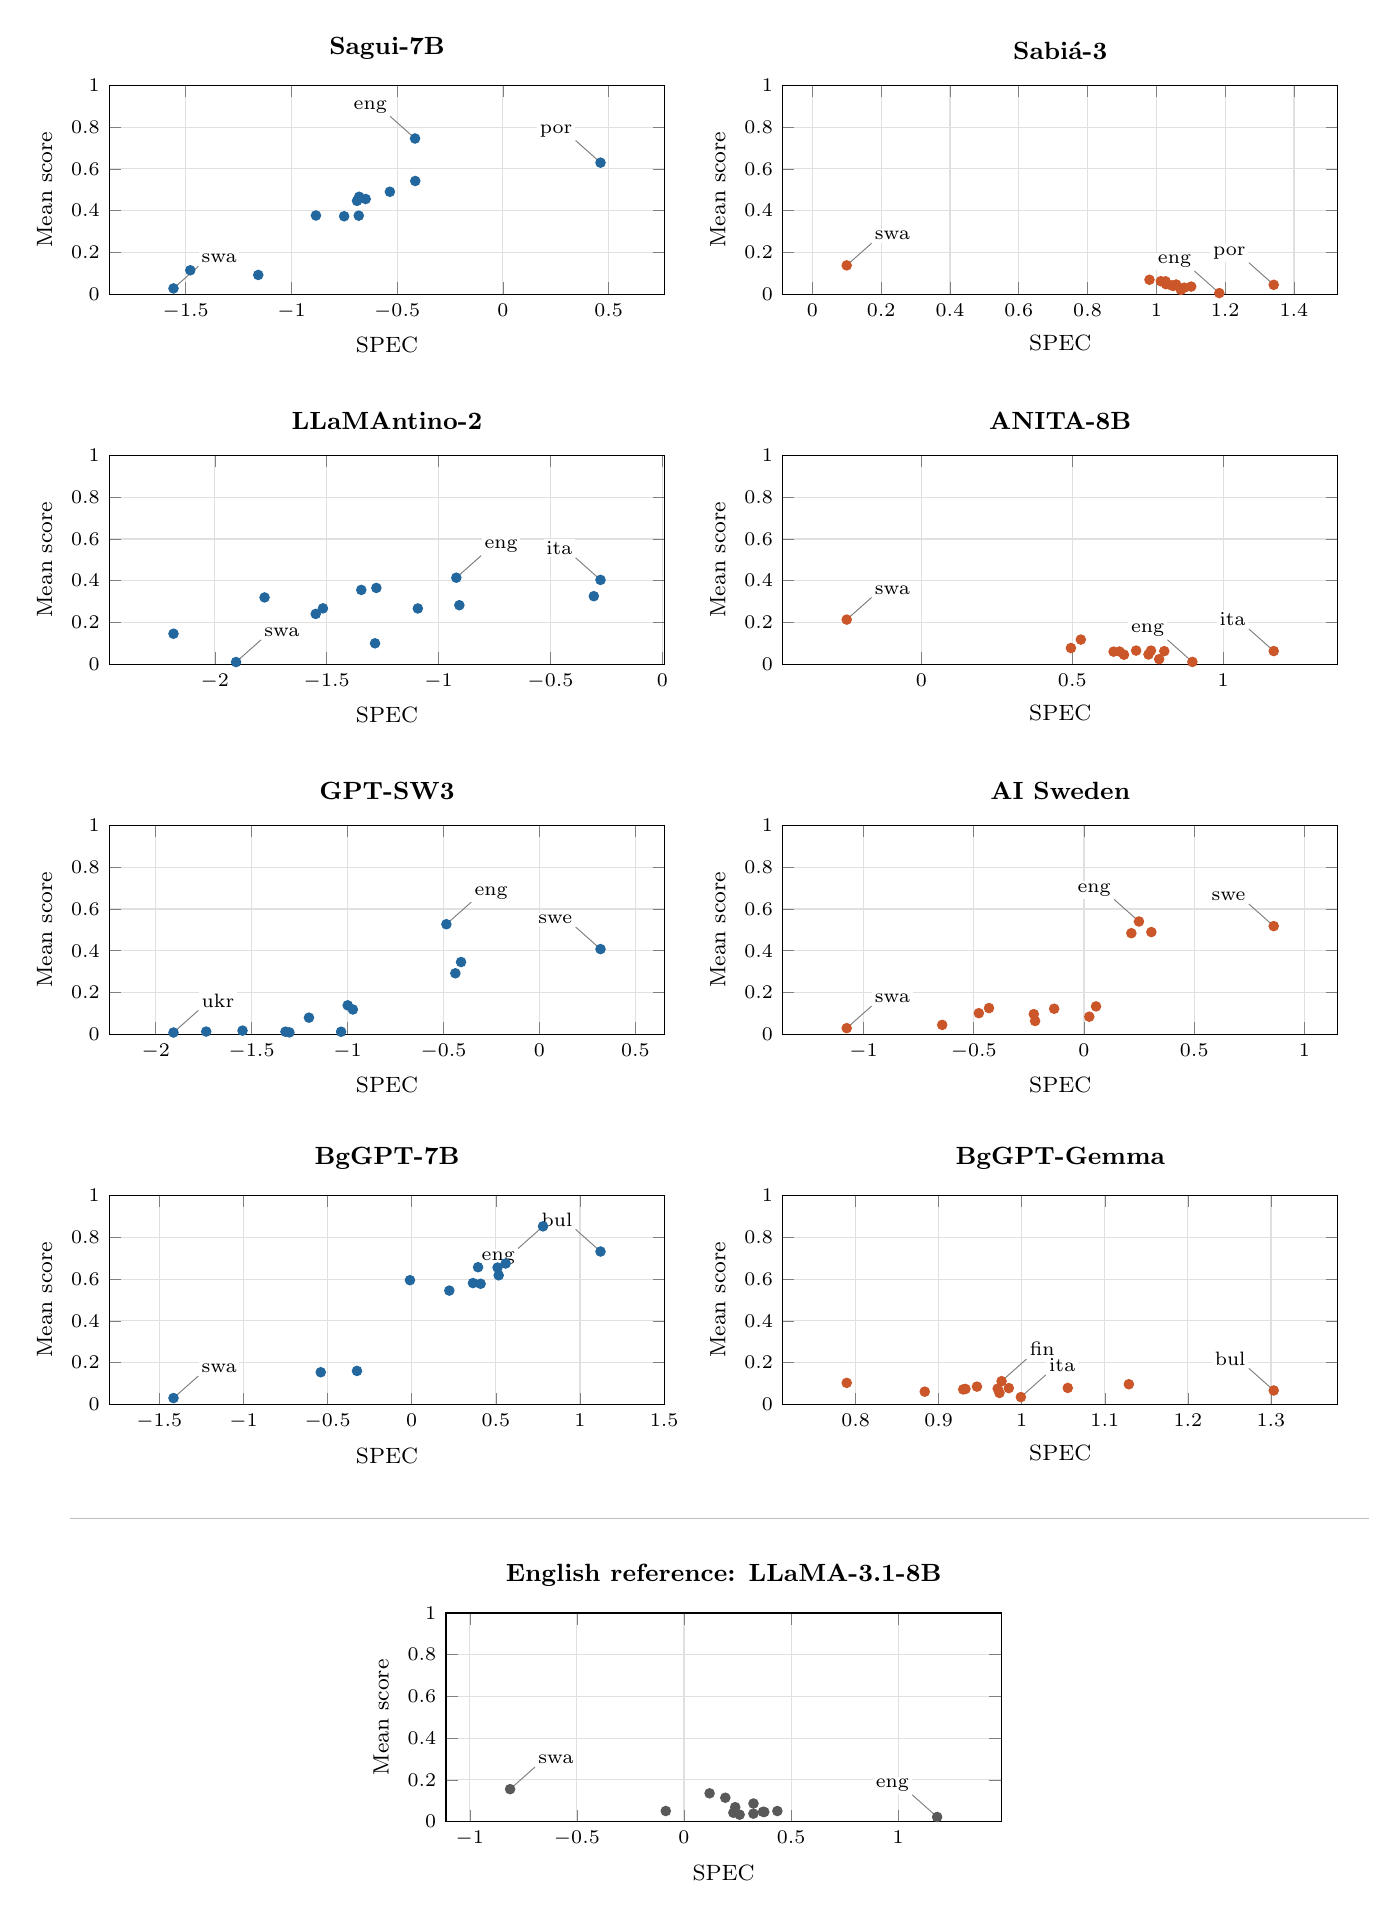
\begin{tikzpicture}
\pgfplotsset{srscatter/.style={width=7.05cm,height=2.65cm,scale only axis,ymin=0,ymax=1,ytick={0,.2,.4,.6,.8,1},xlabel={SPEC},ylabel={Mean score},axis lines=box,grid=major,grid style={black!12},tick label style={font=\scriptsize},label style={font=\footnotesize},title style={font=\bfseries\small},enlarge x limits=.15}}
\begin{axis}[srscatter,at={(0.0cm,-0.0cm)},anchor=north west,title={Sagui-7B}]
\addplot[only marks,color=srweak,mark=*,mark size=1.7pt] coordinates {(0.461719,0.629808) (-0.534344,0.490415) (-0.681593,0.375804) (-0.414341,0.541933) (-0.750621,0.372937) (-0.415355,0.745607) (-1.156874,0.091724) (-0.648837,0.455529) (-0.689740,0.446774) (-1.557684,0.027104) (-0.679633,0.466346) (-1.478279,0.114078) (-0.884044,0.376608)};
\node[font=\scriptsize,anchor=south east,xshift=-9pt,yshift=8pt,fill=white,inner sep=1pt] (languageLabel0) at (axis cs:0.461719,0.629808) {por};
\draw[black!50,line width=.35pt] (languageLabel0.south east) -- (axis cs:0.461719,0.629808);
\node[font=\scriptsize,anchor=south east,xshift=-9pt,yshift=8pt,fill=white,inner sep=1pt] (languageLabel1) at (axis cs:-0.415355,0.745607) {eng};
\draw[black!50,line width=.35pt] (languageLabel1.south east) -- (axis cs:-0.415355,0.745607);
\node[font=\scriptsize,anchor=south west,xshift=9pt,yshift=8pt,fill=white,inner sep=1pt] (languageLabel2) at (axis cs:-1.557684,0.027104) {swa};
\draw[black!50,line width=.35pt] (languageLabel2.south west) -- (axis cs:-1.557684,0.027104);
\end{axis}
\begin{axis}[srscatter,at={(8.55cm,-0.0cm)},anchor=north west,title={Sabi\'a-3}]
\addplot[only marks,color=srstrong,mark=*,mark size=1.7pt] coordinates {(1.341249,0.044471) (1.071393,0.019968) (1.057568,0.045820) (1.080968,0.030751) (1.049015,0.039191) (1.182979,0.004792) (0.980022,0.068686) (1.101309,0.036058) (1.012947,0.061694) (0.099809,0.137540) (1.044153,0.041935) (1.027922,0.047330) (1.026637,0.061093)};
\node[font=\scriptsize,anchor=south east,xshift=-9pt,yshift=8pt,fill=white,inner sep=1pt] (languageLabel0) at (axis cs:1.341249,0.044471) {por};
\draw[black!50,line width=.35pt] (languageLabel0.south east) -- (axis cs:1.341249,0.044471);
\node[font=\scriptsize,anchor=south east,xshift=-9pt,yshift=8pt,fill=white,inner sep=1pt] (languageLabel1) at (axis cs:1.182979,0.004792) {eng};
\draw[black!50,line width=.35pt] (languageLabel1.south east) -- (axis cs:1.182979,0.004792);
\node[font=\scriptsize,anchor=south west,xshift=9pt,yshift=8pt,fill=white,inner sep=1pt] (languageLabel2) at (axis cs:0.099809,0.137540) {swa};
\draw[black!50,line width=.35pt] (languageLabel2.south west) -- (axis cs:0.099809,0.137540);
\end{axis}
\begin{axis}[srscatter,at={(0.0cm,-4.7cm)},anchor=north west,title={LLaMAntino-2}]
\addplot[only marks,color=srweak,mark=*,mark size=1.7pt] coordinates {(-0.276208,0.403754) (-1.277911,0.365354) (-1.777672,0.319719) (-1.345337,0.355769) (-1.548931,0.240756) (-0.306124,0.325721) (-0.920645,0.414263) (-2.184595,0.145904) (-1.516673,0.267395) (-1.904936,0.010113) (-0.907046,0.282556) (-1.283832,0.099919) (-1.092590,0.266935)};
\node[font=\scriptsize,anchor=south east,xshift=-9pt,yshift=8pt,fill=white,inner sep=1pt] (languageLabel0) at (axis cs:-0.276208,0.403754) {ita};
\draw[black!50,line width=.35pt] (languageLabel0.south east) -- (axis cs:-0.276208,0.403754);
\node[font=\scriptsize,anchor=south west,xshift=9pt,yshift=8pt,fill=white,inner sep=1pt] (languageLabel1) at (axis cs:-0.920645,0.414263) {eng};
\draw[black!50,line width=.35pt] (languageLabel1.south west) -- (axis cs:-0.920645,0.414263);
\node[font=\scriptsize,anchor=south west,xshift=9pt,yshift=8pt,fill=white,inner sep=1pt] (languageLabel2) at (axis cs:-1.904936,0.010113) {swa};
\draw[black!50,line width=.35pt] (languageLabel2.south west) -- (axis cs:-1.904936,0.010113);
\end{axis}
\begin{axis}[srscatter,at={(8.55cm,-4.7cm)},anchor=north west,title={ANITA-8B}]
\addplot[only marks,color=srstrong,mark=*,mark size=1.7pt] coordinates {(1.167736,0.062700) (0.760839,0.064904) (0.671355,0.045380) (0.804886,0.062300) (0.711655,0.065113) (0.787907,0.024038) (0.898047,0.010783) (0.528236,0.117747) (0.752557,0.046371) (-0.247794,0.213592) (0.656386,0.060497) (0.495481,0.077265) (0.636848,0.059887)};
\node[font=\scriptsize,anchor=south east,xshift=-9pt,yshift=8pt,fill=white,inner sep=1pt] (languageLabel0) at (axis cs:1.167736,0.062700) {ita};
\draw[black!50,line width=.35pt] (languageLabel0.south east) -- (axis cs:1.167736,0.062700);
\node[font=\scriptsize,anchor=south east,xshift=-9pt,yshift=8pt,fill=white,inner sep=1pt] (languageLabel1) at (axis cs:0.898047,0.010783) {eng};
\draw[black!50,line width=.35pt] (languageLabel1.south east) -- (axis cs:0.898047,0.010783);
\node[font=\scriptsize,anchor=south west,xshift=9pt,yshift=8pt,fill=white,inner sep=1pt] (languageLabel2) at (axis cs:-0.247794,0.213592) {swa};
\draw[black!50,line width=.35pt] (languageLabel2.south west) -- (axis cs:-0.247794,0.213592);
\end{axis}
\begin{axis}[srscatter,at={(0.0cm,-9.4cm)},anchor=north west,title={GPT-SW3}]
\addplot[only marks,color=srweak,mark=*,mark size=1.7pt] coordinates {(0.318123,0.408065) (-0.438340,0.292067) (-0.408694,0.346061) (-1.033724,0.011945) (-0.485024,0.527157) (-0.972369,0.118590) (-1.547373,0.017283) (-1.907215,0.008251) (-1.201291,0.079473) (-1.736743,0.012821) (-0.999245,0.138578) (-1.323659,0.012136) (-1.303106,0.008900)};
\node[font=\scriptsize,anchor=south east,xshift=-9pt,yshift=8pt,fill=white,inner sep=1pt] (languageLabel0) at (axis cs:0.318123,0.408065) {swe};
\draw[black!50,line width=.35pt] (languageLabel0.south east) -- (axis cs:0.318123,0.408065);
\node[font=\scriptsize,anchor=south west,xshift=9pt,yshift=8pt,fill=white,inner sep=1pt] (languageLabel1) at (axis cs:-0.485024,0.527157) {eng};
\draw[black!50,line width=.35pt] (languageLabel1.south west) -- (axis cs:-0.485024,0.527157);
\node[font=\scriptsize,anchor=south west,xshift=9pt,yshift=8pt,fill=white,inner sep=1pt] (languageLabel2) at (axis cs:-1.907215,0.008251) {ukr};
\draw[black!50,line width=.35pt] (languageLabel2.south west) -- (axis cs:-1.907215,0.008251);
\end{axis}
\begin{axis}[srscatter,at={(8.55cm,-9.4cm)},anchor=north west,title={AI Sweden}]
\addplot[only marks,color=srstrong,mark=*,mark size=1.7pt] coordinates {(0.860599,0.518145) (0.305513,0.489583) (0.214828,0.484274) (-0.643025,0.044795) (0.249262,0.540335) (0.024003,0.084135) (-0.476834,0.100884) (-0.430727,0.125413) (-0.221643,0.063498) (-0.135220,0.122196) (0.054674,0.133387) (-0.227663,0.096278) (-1.076084,0.029126)};
\node[font=\scriptsize,anchor=south east,xshift=-9pt,yshift=8pt,fill=white,inner sep=1pt] (languageLabel0) at (axis cs:0.860599,0.518145) {swe};
\draw[black!50,line width=.35pt] (languageLabel0.south east) -- (axis cs:0.860599,0.518145);
\node[font=\scriptsize,anchor=south east,xshift=-9pt,yshift=8pt,fill=white,inner sep=1pt] (languageLabel1) at (axis cs:0.249262,0.540335) {eng};
\draw[black!50,line width=.35pt] (languageLabel1.south east) -- (axis cs:0.249262,0.540335);
\node[font=\scriptsize,anchor=south west,xshift=9pt,yshift=8pt,fill=white,inner sep=1pt] (languageLabel2) at (axis cs:-1.076084,0.029126) {swa};
\draw[black!50,line width=.35pt] (languageLabel2.south west) -- (axis cs:-1.076084,0.029126);
\end{axis}
\begin{axis}[srscatter,at={(0.0cm,-14.1cm)},anchor=north west,title={BgGPT-7B}]
\addplot[only marks,color=srweak,mark=*,mark size=1.7pt] coordinates {(1.121865,0.732315) (0.394273,0.657051) (0.516845,0.618189) (-0.325170,0.159983) (-0.010458,0.594884) (0.409383,0.577724) (0.510152,0.655351) (0.780344,0.853035) (0.558322,0.674920) (0.364052,0.581048) (-0.540499,0.153722) (0.223530,0.545016) (-1.415608,0.029935)};
\node[font=\scriptsize,anchor=south east,xshift=-9pt,yshift=8pt,fill=white,inner sep=1pt] (languageLabel0) at (axis cs:1.121865,0.732315) {bul};
\draw[black!50,line width=.35pt] (languageLabel0.south east) -- (axis cs:1.121865,0.732315);
\node[font=\scriptsize,anchor=north east,xshift=-9pt,yshift=-8pt,fill=white,inner sep=1pt] (languageLabel1) at (axis cs:0.780344,0.853035) {eng};
\draw[black!50,line width=.35pt] (languageLabel1.north east) -- (axis cs:0.780344,0.853035);
\node[font=\scriptsize,anchor=south west,xshift=9pt,yshift=8pt,fill=white,inner sep=1pt] (languageLabel2) at (axis cs:-1.415608,0.029935) {swa};
\draw[black!50,line width=.35pt] (languageLabel2.south west) -- (axis cs:-1.415608,0.029935);
\end{axis}
\begin{axis}[srscatter,at={(8.55cm,-14.1cm)},anchor=north west,title={BgGPT-Gemma}]
\addplot[only marks,color=srstrong,mark=*,mark size=1.7pt] coordinates {(1.303355,0.066318) (0.973194,0.054487) (0.984450,0.077724) (0.975763,0.110922) (0.929587,0.071370) (1.055438,0.078526) (0.998986,0.034744) (1.128961,0.096246) (0.971064,0.075080) (0.932291,0.073651) (0.883276,0.060680) (0.946117,0.084807) (0.789336,0.102751)};
\node[font=\scriptsize,anchor=south east,xshift=-9pt,yshift=8pt,fill=white,inner sep=1pt] (languageLabel0) at (axis cs:1.303355,0.066318) {bul};
\draw[black!50,line width=.35pt] (languageLabel0.south east) -- (axis cs:1.303355,0.066318);
\node[font=\scriptsize,anchor=south west,xshift=9pt,yshift=8pt,fill=white,inner sep=1pt] (languageLabel1) at (axis cs:0.975763,0.110922) {fin};
\draw[black!50,line width=.35pt] (languageLabel1.south west) -- (axis cs:0.975763,0.110922);
\node[font=\scriptsize,anchor=south west,xshift=9pt,yshift=8pt,fill=white,inner sep=1pt] (languageLabel2) at (axis cs:0.998986,0.034744) {ita};
\draw[black!50,line width=.35pt] (languageLabel2.south west) -- (axis cs:0.998986,0.034744);
\end{axis}
\draw[black!25] (-.5,-18.2) -- (16,-18.2);
\begin{axis}[srscatter,at={(4.275cm,-19.4cm)},anchor=north west,title={English reference: LLaMA-3.1-8B}]
\addplot[only marks,color=black!65,mark=*,mark size=1.7pt] coordinates {(1.181697,0.022364) (0.324334,0.086939) (0.239115,0.069311) (0.368920,0.047026) (0.374768,0.046371) (0.192872,0.114550) (0.259633,0.033416) (0.324048,0.038339) (0.119382,0.135666) (0.230438,0.042732) (-0.084995,0.050971) (0.435809,0.050881) (-0.811875,0.155744)};
\node[font=\scriptsize,anchor=south east,xshift=-9pt,yshift=8pt,fill=white,inner sep=1pt] (languageLabel0) at (axis cs:1.181697,0.022364) {eng};
\draw[black!50,line width=.35pt] (languageLabel0.south east) -- (axis cs:1.181697,0.022364);
\node[font=\scriptsize,anchor=south west,xshift=9pt,yshift=8pt,fill=white,inner sep=1pt] (languageLabel1) at (axis cs:-0.811875,0.155744) {swa};
\draw[black!50,line width=.35pt] (languageLabel1.south west) -- (axis cs:-0.811875,0.155744);
\end{axis}
\end{tikzpicture}
\end{adjustbox}
\caption{BELEBELE specialization and mean StrongREJECT score in the observed model--language cells. The four paired rows are followed by a separate English-reference panel, which is descriptive and excluded from paired inference. Language labels identify the aligned language and the lowest and highest mean StrongREJECT scores within each model.}\label{fig:graded-spec}\fonte{Author.}
\end{figure}
The different appearance of LLaMAntino-2 in Figure~\ref{fig:belebele-profiles} reflects limited comparable answers, rather than a different plotting method. CONS has 95\% Wilson intervals for every model; the intervals for other models are generally narrower and therefore less conspicuous. LLaMAntino-2 has few parseable aligned-language answers, which limits the number of questions that can be compared across languages and makes its CONS intervals much wider. Hollow points identify cells with fewer than 100 comparable answers. We leave those CONS points, and the SPEC values that depend on them, disconnected so that the figure does not suggest a reliably measured language curve. The intervals quantify uncertainty conditional on the parseable pairs; they do not correct for missing or unparsed answers.

\begin{figure}[p]\centering
\begin{adjustbox}{max totalsize={\linewidth}{.65\textheight},center}% Reference extension by eval/scripts/write_reference_comparison_figures.py.
% Generated by eval/scripts/write_belebele_profiles.py; released scores unchanged.
\definecolor{belebeleif}{RGB}{35,103,159}
\definecolor{belebelecons}{RGB}{202,86,42}
\definecolor{belebelespec}{RGB}{38,132,109}
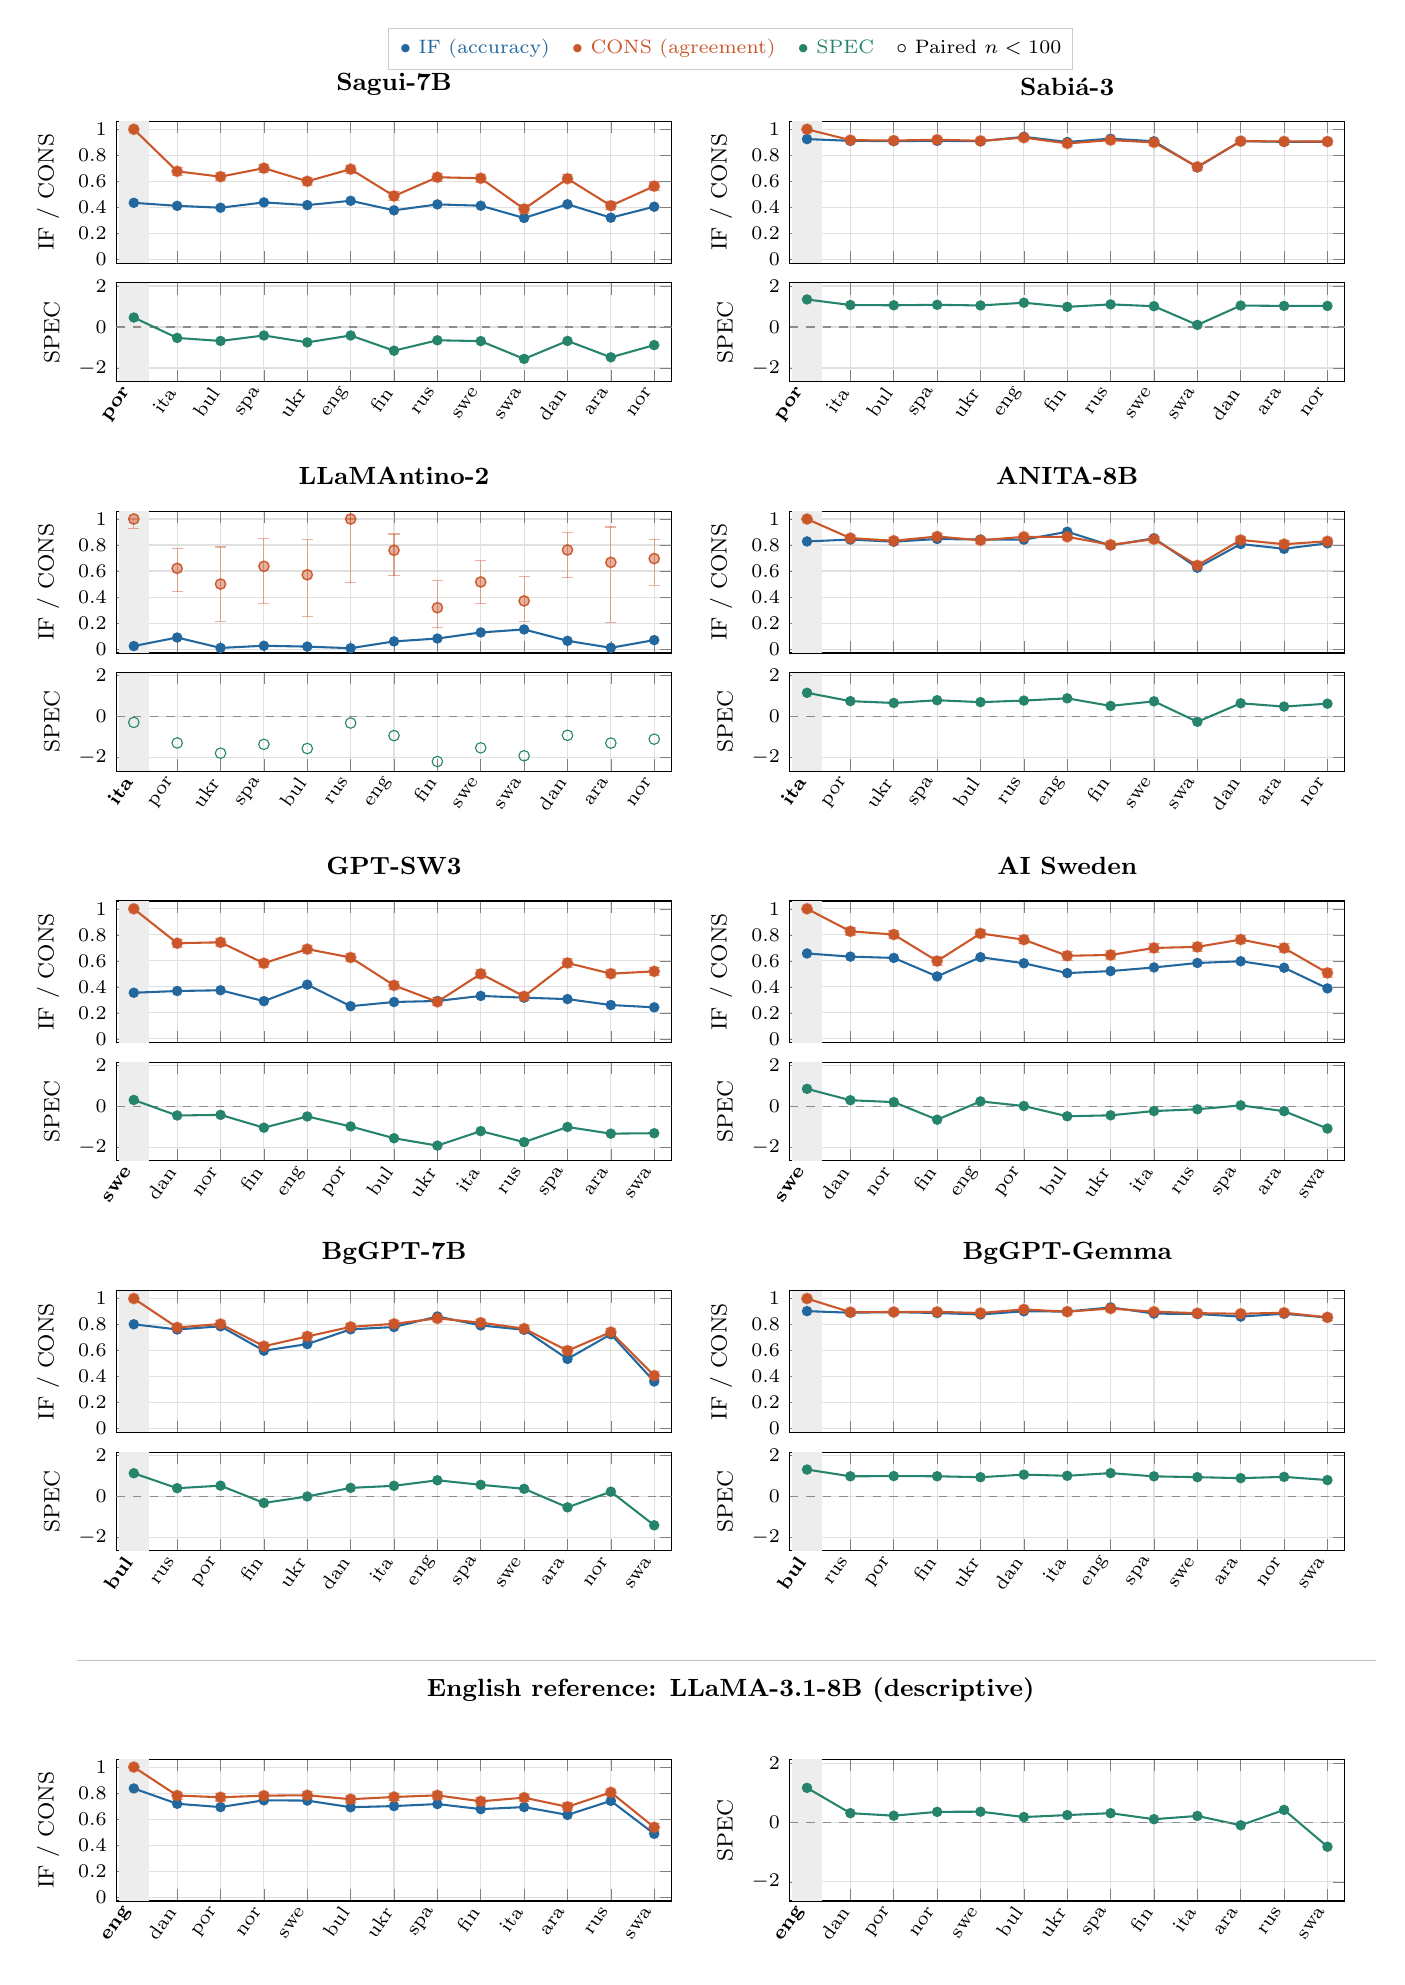
\begin{tikzpicture}
\pgfplotsset{belebeleaxis/.style={width=7.05cm,scale only axis,xmin=-.4,xmax=12.4,
axis lines=box,grid=major,grid style={black!12},
tick label style={font=\scriptsize},label style={font=\footnotesize},
title style={font=\bfseries\small},unbounded coords=jump,
clip=true,xtick={0,...,12}}}
\node[anchor=south,draw=black!20,fill=white,inner sep=4pt,font=\scriptsize] at (7.8,.65) {\textcolor{belebeleif}{$\bullet$ IF (accuracy)}\quad
\textcolor{belebelecons}{$\bullet$ CONS (agreement)}\quad
\textcolor{belebelespec}{$\bullet$ SPEC}\quad $\circ$ Paired $n<100$};
\begin{axis}[belebeleaxis,height=1.8cm,at={(0.00cm,0.00cm)},anchor=north west,
title={Sagui-7B},
ymin=-.03,ymax=1.06,ytick={0,.2,.4,.6,.8,1},xticklabels=\empty,ylabel={IF / CONS}]
\path[fill=black!7] (axis cs:-.35,-.03) rectangle (axis cs:.35,1.06);
\addplot[color=belebeleif,mark=*,mark size=1.5pt,line width=.75pt] coordinates {(0,0.434444) (1,0.411111) (2,0.396667) (3,0.437778) (4,0.416667) (5,0.450000) (6,0.376667) (7,0.422222) (8,0.412222) (9,0.317778) (10,0.423333) (11,0.320000) (12,0.404444)};
\addplot[color=belebelecons,mark=*,mark size=1.5pt,line width=.75pt] coordinates {(0,1.000000) (1,0.676667) (2,0.635556) (3,0.701111) (4,0.600000) (5,0.693333) (6,0.486667) (7,0.631111) (8,0.623333) (9,0.386667) (10,0.620000) (11,0.412222) (12,0.562222)};
\addplot[color=belebelecons,opacity=.45,only marks,mark=none,error bars/.cd,y dir=both,y explicit] coordinates {(0,1.000000) += (0,0.000000) -= (0,0.004250) (1,0.676667) += (0,0.029752) -= (0,0.031254) (2,0.635556) += (0,0.030805) -= (0,0.031957) (3,0.701111) += (0,0.029001) -= (0,0.030711) (4,0.600000) += (0,0.031516) -= (0,0.032366) (5,0.693333) += (0,0.029251) -= (0,0.030894) (6,0.486667) += (0,0.032642) -= (0,0.032528) (7,0.631111) += (0,0.030904) -= (0,0.032018) (8,0.623333) += (0,0.031070) -= (0,0.032118) (9,0.386667) += (0,0.032234) -= (0,0.031270) (10,0.620000) += (0,0.031138) -= (0,0.032158) (11,0.412222) += (0,0.032466) -= (0,0.031719) (12,0.562222) += (0,0.032080) -= (0,0.032609)};
\addplot[color=belebelecons,only marks,mark=o,mark options={fill=white},mark size=1.8pt] coordinates {            };
\end{axis}
\begin{axis}[belebeleaxis,height=1.25cm,at={(0.00cm,-2.05cm)},anchor=north west,
ymin=-2.65,ymax=2.15,ytick={-2,0,2},xticklabels={\textbf{por},ita,bul,spa,ukr,eng,fin,rus,swe,swa,dan,ara,nor},x tick label style={rotate=55,anchor=east,font=\scriptsize},ylabel={SPEC}]
\path[fill=black!7] (axis cs:-.35,-2.65) rectangle (axis cs:.35,2.15);
\addplot[black!45,dashed,mark=none] coordinates {(-.4,0) (12.4,0)};
\addplot[color=belebelespec,mark=*,mark size=1.5pt,line width=.75pt] coordinates {(0,0.461719) (1,-0.534344) (2,-0.681593) (3,-0.414341) (4,-0.750621) (5,-0.415355) (6,-1.156874) (7,-0.648837) (8,-0.689740) (9,-1.557684) (10,-0.679633) (11,-1.478279) (12,-0.884044)};
\addplot[color=belebelespec,only marks,mark=o,mark options={fill=white},mark size=1.9pt] coordinates {            };
\end{axis}
\begin{axis}[belebeleaxis,height=1.8cm,at={(8.55cm,0.00cm)},anchor=north west,
title={Sabi\'a-3},
ymin=-.03,ymax=1.06,ytick={0,.2,.4,.6,.8,1},xticklabels=\empty,ylabel={IF / CONS}]
\path[fill=black!7] (axis cs:-.35,-.03) rectangle (axis cs:.35,1.06);
\addplot[color=belebeleif,mark=*,mark size=1.5pt,line width=.75pt] coordinates {(0,0.924444) (1,0.911111) (2,0.908889) (3,0.911111) (4,0.907778) (5,0.942222) (6,0.902222) (7,0.927778) (8,0.907778) (9,0.707778) (10,0.908889) (11,0.903333) (12,0.904444)};
\addplot[color=belebelecons,mark=*,mark size=1.5pt,line width=.75pt] coordinates {(0,1.000000) (1,0.916667) (2,0.913333) (3,0.919911) (4,0.911111) (5,0.935556) (6,0.891111) (7,0.916667) (8,0.898889) (9,0.711111) (10,0.908788) (11,0.906667) (12,0.905556)};
\addplot[color=belebelecons,opacity=.45,only marks,mark=none,error bars/.cd,y dir=both,y explicit] coordinates {(0,1.000000) += (0,0.000000) -= (0,0.004250) (1,0.916667) += (0,0.016334) -= (0,0.019876) (2,0.913333) += (0,0.016669) -= (0,0.020182) (3,0.919911) += (0,0.016008) -= (0,0.019582) (4,0.911111) += (0,0.016888) -= (0,0.020382) (5,0.935556) += (0,0.014263) -= (0,0.017966) (6,0.891111) += (0,0.018713) -= (0,0.022038) (7,0.916667) += (0,0.016334) -= (0,0.019876) (8,0.898889) += (0,0.018032) -= (0,0.021422) (9,0.711111) += (0,0.028665) -= (0,0.030459) (10,0.908788) += (0,0.017121) -= (0,0.020600) (11,0.906667) += (0,0.017315) -= (0,0.020772) (12,0.905556) += (0,0.017420) -= (0,0.020867)};
\addplot[color=belebelecons,only marks,mark=o,mark options={fill=white},mark size=1.8pt] coordinates {            };
\end{axis}
\begin{axis}[belebeleaxis,height=1.25cm,at={(8.55cm,-2.05cm)},anchor=north west,
ymin=-2.65,ymax=2.15,ytick={-2,0,2},xticklabels={\textbf{por},ita,bul,spa,ukr,eng,fin,rus,swe,swa,dan,ara,nor},x tick label style={rotate=55,anchor=east,font=\scriptsize},ylabel={SPEC}]
\path[fill=black!7] (axis cs:-.35,-2.65) rectangle (axis cs:.35,2.15);
\addplot[black!45,dashed,mark=none] coordinates {(-.4,0) (12.4,0)};
\addplot[color=belebelespec,mark=*,mark size=1.5pt,line width=.75pt] coordinates {(0,1.341249) (1,1.071393) (2,1.057568) (3,1.080968) (4,1.049015) (5,1.182979) (6,0.980022) (7,1.101309) (8,1.012947) (9,0.099809) (10,1.044153) (11,1.027922) (12,1.026637)};
\addplot[color=belebelespec,only marks,mark=o,mark options={fill=white},mark size=1.9pt] coordinates {            };
\end{axis}
\begin{axis}[belebeleaxis,height=1.8cm,at={(0.00cm,-4.95cm)},anchor=north west,
title={LLaMAntino-2},
ymin=-.03,ymax=1.06,ytick={0,.2,.4,.6,.8,1},xticklabels=\empty,ylabel={IF / CONS}]
\path[fill=black!7] (axis cs:-.35,-.03) rectangle (axis cs:.35,1.06);
\addplot[color=belebeleif,mark=*,mark size=1.5pt,line width=.75pt] coordinates {(0,0.023333) (1,0.088889) (2,0.008889) (3,0.025556) (4,0.018889) (5,0.006667) (6,0.058889) (7,0.081111) (8,0.127778) (9,0.151111) (10,0.063333) (11,0.010000) (12,0.068889)};
\addplot[color=belebelecons,mark=*,mark size=1.5pt,line width=.75pt] coordinates {(0,nan) (1,nan) (2,nan) (3,nan) (4,nan) (5,nan) (6,nan) (7,nan) (8,nan) (9,nan) (10,nan) (11,nan) (12,nan)};
\addplot[color=belebelecons,opacity=.45,only marks,mark=none,error bars/.cd,y dir=both,y explicit] coordinates {(0,1.000000) += (0,0.000000) -= (0,0.071348) (1,0.620690) += (0,0.152430) -= (0,0.180664) (2,0.500000) += (0,0.284784) -= (0,0.284784) (3,0.636364) += (0,0.211972) -= (0,0.282562) (4,0.571429) += (0,0.270352) -= (0,0.320970) (5,1.000000) += (0,0.000000) -= (0,0.489891) (6,0.760000) += (0,0.125037) -= (0,0.194297) (7,0.318182) += (0,0.208632) -= (0,0.154576) (8,0.516129) += (0,0.164168) -= (0,0.167725) (9,0.370370) += (0,0.187337) -= (0,0.155045) (10,0.761905) += (0,0.131815) -= (0,0.212816) (11,0.666667) += (0,0.271841) -= (0,0.459007) (12,0.695652) += (0,0.148308) -= (0,0.204310)};
\addplot[color=belebelecons,only marks,mark=o,mark options={fill=white},mark size=1.8pt] coordinates {(0,1.000000) (1,0.620690) (2,0.500000) (3,0.636364) (4,0.571429) (5,1.000000) (6,0.760000) (7,0.318182) (8,0.516129) (9,0.370370) (10,0.761905) (11,0.666667) (12,0.695652)};
\end{axis}
\begin{axis}[belebeleaxis,height=1.25cm,at={(0.00cm,-7.00cm)},anchor=north west,
ymin=-2.65,ymax=2.15,ytick={-2,0,2},xticklabels={\textbf{ita},por,ukr,spa,bul,rus,eng,fin,swe,swa,dan,ara,nor},x tick label style={rotate=55,anchor=east,font=\scriptsize},ylabel={SPEC}]
\path[fill=black!7] (axis cs:-.35,-2.65) rectangle (axis cs:.35,2.15);
\addplot[black!45,dashed,mark=none] coordinates {(-.4,0) (12.4,0)};
\addplot[color=belebelespec,mark=*,mark size=1.5pt,line width=.75pt] coordinates {(0,nan) (1,nan) (2,nan) (3,nan) (4,nan) (5,nan) (6,nan) (7,nan) (8,nan) (9,nan) (10,nan) (11,nan) (12,nan)};
\addplot[color=belebelespec,only marks,mark=o,mark options={fill=white},mark size=1.9pt] coordinates {(0,-0.276208) (1,-1.277911) (2,-1.777672) (3,-1.345337) (4,-1.548931) (5,-0.306124) (6,-0.920645) (7,-2.184595) (8,-1.516673) (9,-1.904936) (10,-0.907046) (11,-1.283832) (12,-1.092590)};
\end{axis}
\begin{axis}[belebeleaxis,height=1.8cm,at={(8.55cm,-4.95cm)},anchor=north west,
title={ANITA-8B},
ymin=-.03,ymax=1.06,ytick={0,.2,.4,.6,.8,1},xticklabels=\empty,ylabel={IF / CONS}]
\path[fill=black!7] (axis cs:-.35,-.03) rectangle (axis cs:.35,1.06);
\addplot[color=belebeleif,mark=*,mark size=1.5pt,line width=.75pt] coordinates {(0,0.827778) (1,0.842222) (2,0.825556) (3,0.846667) (4,0.842222) (5,0.841111) (6,0.902222) (7,0.796667) (8,0.852222) (9,0.625556) (10,0.807778) (11,0.771111) (12,0.813333)};
\addplot[color=belebelecons,mark=*,mark size=1.5pt,line width=.75pt] coordinates {(0,1.000000) (1,0.853333) (2,0.833148) (3,0.865556) (4,0.836667) (5,0.863181) (6,0.863333) (7,0.802222) (8,0.844444) (9,0.643333) (10,0.838889) (11,0.806667) (12,0.828889)};
\addplot[color=belebelecons,opacity=.45,only marks,mark=none,error bars/.cd,y dir=both,y explicit] coordinates {(0,1.000000) += (0,0.000000) -= (0,0.004250) (1,0.853333) += (0,0.021611) -= (0,0.024614) (2,0.833148) += (0,0.022944) -= (0,0.025779) (3,0.865556) += (0,0.020740) -= (0,0.023847) (4,0.836667) += (0,0.022711) -= (0,0.025573) (5,0.863181) += (0,0.020924) -= (0,0.024015) (6,0.863333) += (0,0.020902) -= (0,0.023991) (7,0.802222) += (0,0.024715) -= (0,0.027284) (8,0.844444) += (0,0.022210) -= (0,0.025137) (9,0.643333) += (0,0.030625) -= (0,0.031844) (10,0.838889) += (0,0.022570) -= (0,0.025451) (11,0.806667) += (0,0.024475) -= (0,0.027082) (12,0.828889) += (0,0.023194) -= (0,0.025990)};
\addplot[color=belebelecons,only marks,mark=o,mark options={fill=white},mark size=1.8pt] coordinates {            };
\end{axis}
\begin{axis}[belebeleaxis,height=1.25cm,at={(8.55cm,-7.00cm)},anchor=north west,
ymin=-2.65,ymax=2.15,ytick={-2,0,2},xticklabels={\textbf{ita},por,ukr,spa,bul,rus,eng,fin,swe,swa,dan,ara,nor},x tick label style={rotate=55,anchor=east,font=\scriptsize},ylabel={SPEC}]
\path[fill=black!7] (axis cs:-.35,-2.65) rectangle (axis cs:.35,2.15);
\addplot[black!45,dashed,mark=none] coordinates {(-.4,0) (12.4,0)};
\addplot[color=belebelespec,mark=*,mark size=1.5pt,line width=.75pt] coordinates {(0,1.167736) (1,0.760839) (2,0.671355) (3,0.804886) (4,0.711655) (5,0.787907) (6,0.898047) (7,0.528236) (8,0.752557) (9,-0.247794) (10,0.656386) (11,0.495481) (12,0.636848)};
\addplot[color=belebelespec,only marks,mark=o,mark options={fill=white},mark size=1.9pt] coordinates {            };
\end{axis}
\begin{axis}[belebeleaxis,height=1.8cm,at={(0.00cm,-9.90cm)},anchor=north west,
title={GPT-SW3},
ymin=-.03,ymax=1.06,ytick={0,.2,.4,.6,.8,1},xticklabels=\empty,ylabel={IF / CONS}]
\path[fill=black!7] (axis cs:-.35,-.03) rectangle (axis cs:.35,1.06);
\addplot[color=belebeleif,mark=*,mark size=1.5pt,line width=.75pt] coordinates {(0,0.354444) (1,0.367778) (2,0.373333) (3,0.290000) (4,0.416667) (5,0.251111) (6,0.283333) (7,0.291111) (8,0.330000) (9,0.316667) (10,0.305556) (11,0.260000) (12,0.242222)};
\addplot[color=belebelecons,mark=*,mark size=1.5pt,line width=.75pt] coordinates {(0,1.000000) (1,0.735556) (2,0.742222) (3,0.581111) (4,0.690000) (5,0.625556) (6,0.411111) (7,0.284444) (8,0.500000) (9,0.326667) (10,0.583333) (11,0.501111) (12,0.518889)};
\addplot[color=belebelecons,opacity=.45,only marks,mark=none,error bars/.cd,y dir=both,y explicit] coordinates {(0,1.000000) += (0,0.000000) -= (0,0.004250) (1,0.735556) += (0,0.027769) -= (0,0.029771) (2,0.742222) += (0,0.027505) -= (0,0.029564) (3,0.581111) += (0,0.031822) -= (0,0.032511) (4,0.690000) += (0,0.029355) -= (0,0.030970) (5,0.625556) += (0,0.031023) -= (0,0.032090) (6,0.411111) += (0,0.032457) -= (0,0.031702) (7,0.284444) += (0,0.030342) -= (0,0.028510) (8,0.500000) += (0,0.032597) -= (0,0.032597) (9,0.326667) += (0,0.031321) -= (0,0.029847) (10,0.583333) += (0,0.031788) -= (0,0.032497) (11,0.501111) += (0,0.032592) -= (0,0.032601) (12,0.518889) += (0,0.032493) -= (0,0.032654)};
\addplot[color=belebelecons,only marks,mark=o,mark options={fill=white},mark size=1.8pt] coordinates {            };
\end{axis}
\begin{axis}[belebeleaxis,height=1.25cm,at={(0.00cm,-11.95cm)},anchor=north west,
ymin=-2.65,ymax=2.15,ytick={-2,0,2},xticklabels={\textbf{swe},dan,nor,fin,eng,por,bul,ukr,ita,rus,spa,ara,swa},x tick label style={rotate=55,anchor=east,font=\scriptsize},ylabel={SPEC}]
\path[fill=black!7] (axis cs:-.35,-2.65) rectangle (axis cs:.35,2.15);
\addplot[black!45,dashed,mark=none] coordinates {(-.4,0) (12.4,0)};
\addplot[color=belebelespec,mark=*,mark size=1.5pt,line width=.75pt] coordinates {(0,0.318123) (1,-0.438340) (2,-0.408694) (3,-1.033724) (4,-0.485024) (5,-0.972369) (6,-1.547373) (7,-1.907215) (8,-1.201291) (9,-1.736743) (10,-0.999245) (11,-1.323659) (12,-1.303106)};
\addplot[color=belebelespec,only marks,mark=o,mark options={fill=white},mark size=1.9pt] coordinates {            };
\end{axis}
\begin{axis}[belebeleaxis,height=1.8cm,at={(8.55cm,-9.90cm)},anchor=north west,
title={AI Sweden},
ymin=-.03,ymax=1.06,ytick={0,.2,.4,.6,.8,1},xticklabels=\empty,ylabel={IF / CONS}]
\path[fill=black!7] (axis cs:-.35,-.03) rectangle (axis cs:.35,1.06);
\addplot[color=belebeleif,mark=*,mark size=1.5pt,line width=.75pt] coordinates {(0,0.656667) (1,0.632222) (2,0.622222) (3,0.480000) (4,0.627778) (5,0.581111) (6,0.505556) (7,0.521111) (8,0.548889) (9,0.583333) (10,0.596667) (11,0.546667) (12,0.387778)};
\addplot[color=belebelecons,mark=*,mark size=1.5pt,line width=.75pt] coordinates {(0,1.000000) (1,0.826772) (2,0.802125) (3,0.597938) (4,0.810414) (5,0.762467) (6,0.638710) (7,0.644872) (8,0.698827) (9,0.707161) (10,0.763399) (11,0.698138) (12,0.507285)};
\addplot[color=belebelecons,opacity=.45,only marks,mark=none,error bars/.cd,y dir=both,y explicit] coordinates {(0,1.000000) += (0,0.000000) -= (0,0.004755) (1,0.826772) += (0,0.025214) -= (0,0.028492) (2,0.802125) += (0,0.026891) -= (0,0.029958) (3,0.597938) += (0,0.033934) -= (0,0.034899) (4,0.810414) += (0,0.026461) -= (0,0.029628) (5,0.762467) += (0,0.028853) -= (0,0.031486) (6,0.638710) += (0,0.033060) -= (0,0.034428) (7,0.644872) += (0,0.032799) -= (0,0.034219) (8,0.698827) += (0,0.031410) -= (0,0.033392) (9,0.707161) += (0,0.030820) -= (0,0.032845) (10,0.763399) += (0,0.028754) -= (0,0.031386) (11,0.698138) += (0,0.031736) -= (0,0.033750) (12,0.507285) += (0,0.035534) -= (0,0.035608)};
\addplot[color=belebelecons,only marks,mark=o,mark options={fill=white},mark size=1.8pt] coordinates {            };
\end{axis}
\begin{axis}[belebeleaxis,height=1.25cm,at={(8.55cm,-11.95cm)},anchor=north west,
ymin=-2.65,ymax=2.15,ytick={-2,0,2},xticklabels={\textbf{swe},dan,nor,fin,eng,por,bul,ukr,ita,rus,spa,ara,swa},x tick label style={rotate=55,anchor=east,font=\scriptsize},ylabel={SPEC}]
\path[fill=black!7] (axis cs:-.35,-2.65) rectangle (axis cs:.35,2.15);
\addplot[black!45,dashed,mark=none] coordinates {(-.4,0) (12.4,0)};
\addplot[color=belebelespec,mark=*,mark size=1.5pt,line width=.75pt] coordinates {(0,0.860599) (1,0.305513) (2,0.214828) (3,-0.643025) (4,0.249262) (5,0.024003) (6,-0.476834) (7,-0.430727) (8,-0.221643) (9,-0.135220) (10,0.054674) (11,-0.227663) (12,-1.076084)};
\addplot[color=belebelespec,only marks,mark=o,mark options={fill=white},mark size=1.9pt] coordinates {            };
\end{axis}
\begin{axis}[belebeleaxis,height=1.8cm,at={(0.00cm,-14.85cm)},anchor=north west,
title={BgGPT-7B},
ymin=-.03,ymax=1.06,ytick={0,.2,.4,.6,.8,1},xticklabels=\empty,ylabel={IF / CONS}]
\path[fill=black!7] (axis cs:-.35,-.03) rectangle (axis cs:.35,1.06);
\addplot[color=belebeleif,mark=*,mark size=1.5pt,line width=.75pt] coordinates {(0,0.802222) (1,0.762222) (2,0.786667) (3,0.598889) (4,0.650000) (5,0.763333) (6,0.781111) (7,0.862222) (8,0.793333) (9,0.760000) (10,0.535556) (11,0.725556) (12,0.362222)};
\addplot[color=belebelecons,mark=*,mark size=1.5pt,line width=.75pt] coordinates {(0,1.000000) (1,0.777778) (2,0.804444) (3,0.633333) (4,0.708889) (5,0.782222) (6,0.805556) (7,0.847778) (8,0.814444) (9,0.768889) (10,0.598889) (11,0.742222) (12,0.407778)};
\addplot[color=belebelecons,opacity=.45,only marks,mark=none,error bars/.cd,y dir=both,y explicit] coordinates {(0,1.000000) += (0,0.000000) -= (0,0.004250) (1,0.777778) += (0,0.025948) -= (0,0.028310) (2,0.804444) += (0,0.024596) -= (0,0.027184) (3,0.633333) += (0,0.030855) -= (0,0.031988) (4,0.708889) += (0,0.028741) -= (0,0.030517) (5,0.782222) += (0,0.025735) -= (0,0.028134) (6,0.805556) += (0,0.024536) -= (0,0.027133) (7,0.847778) += (0,0.021988) -= (0,0.024944) (8,0.814444) += (0,0.024042) -= (0,0.026715) (9,0.768889) += (0,0.026363) -= (0,0.028648) (10,0.598889) += (0,0.031535) -= (0,0.032376) (11,0.742222) += (0,0.027505) -= (0,0.029564) (12,0.407778) += (0,0.032432) -= (0,0.031648)};
\addplot[color=belebelecons,only marks,mark=o,mark options={fill=white},mark size=1.8pt] coordinates {            };
\end{axis}
\begin{axis}[belebeleaxis,height=1.25cm,at={(0.00cm,-16.90cm)},anchor=north west,
ymin=-2.65,ymax=2.15,ytick={-2,0,2},xticklabels={\textbf{bul},rus,por,fin,ukr,dan,ita,eng,spa,swe,ara,nor,swa},x tick label style={rotate=55,anchor=east,font=\scriptsize},ylabel={SPEC}]
\path[fill=black!7] (axis cs:-.35,-2.65) rectangle (axis cs:.35,2.15);
\addplot[black!45,dashed,mark=none] coordinates {(-.4,0) (12.4,0)};
\addplot[color=belebelespec,mark=*,mark size=1.5pt,line width=.75pt] coordinates {(0,1.121865) (1,0.394273) (2,0.516845) (3,-0.325170) (4,-0.010458) (5,0.409383) (6,0.510152) (7,0.780344) (8,0.558322) (9,0.364052) (10,-0.540499) (11,0.223530) (12,-1.415608)};
\addplot[color=belebelespec,only marks,mark=o,mark options={fill=white},mark size=1.9pt] coordinates {            };
\end{axis}
\begin{axis}[belebeleaxis,height=1.8cm,at={(8.55cm,-14.85cm)},anchor=north west,
title={BgGPT-Gemma},
ymin=-.03,ymax=1.06,ytick={0,.2,.4,.6,.8,1},xticklabels=\empty,ylabel={IF / CONS}]
\path[fill=black!7] (axis cs:-.35,-.03) rectangle (axis cs:.35,1.06);
\addplot[color=belebeleif,mark=*,mark size=1.5pt,line width=.75pt] coordinates {(0,0.903333) (1,0.891111) (2,0.895556) (3,0.888889) (4,0.877778) (5,0.902222) (6,0.900000) (7,0.932222) (8,0.884444) (9,0.881111) (10,0.861111) (11,0.883333) (12,0.854444)};
\addplot[color=belebelecons,mark=*,mark size=1.5pt,line width=.75pt] coordinates {(0,1.000000) (1,0.895556) (2,0.896667) (3,0.897778) (4,0.888889) (5,0.916667) (6,0.898889) (7,0.923333) (8,0.898889) (9,0.887778) (10,0.883333) (11,0.891111) (12,0.855556)};
\addplot[color=belebelecons,opacity=.45,only marks,mark=none,error bars/.cd,y dir=both,y explicit] coordinates {(0,1.000000) += (0,0.000000) -= (0,0.004250) (1,0.895556) += (0,0.018328) -= (0,0.021690) (2,0.896667) += (0,0.018230) -= (0,0.021602) (3,0.897778) += (0,0.018131) -= (0,0.021512) (4,0.888889) += (0,0.018902) -= (0,0.022208) (5,0.916667) += (0,0.016334) -= (0,0.019876) (6,0.898889) += (0,0.018032) -= (0,0.021422) (7,0.923333) += (0,0.015639) -= (0,0.019238) (8,0.898889) += (0,0.018032) -= (0,0.021422) (9,0.887778) += (0,0.018995) -= (0,0.022292) (10,0.883333) += (0,0.019363) -= (0,0.022621) (11,0.891111) += (0,0.018713) -= (0,0.022038) (12,0.855556) += (0,0.021457) -= (0,0.024479)};
\addplot[color=belebelecons,only marks,mark=o,mark options={fill=white},mark size=1.8pt] coordinates {            };
\end{axis}
\begin{axis}[belebeleaxis,height=1.25cm,at={(8.55cm,-16.90cm)},anchor=north west,
ymin=-2.65,ymax=2.15,ytick={-2,0,2},xticklabels={\textbf{bul},rus,por,fin,ukr,dan,ita,eng,spa,swe,ara,nor,swa},x tick label style={rotate=55,anchor=east,font=\scriptsize},ylabel={SPEC}]
\path[fill=black!7] (axis cs:-.35,-2.65) rectangle (axis cs:.35,2.15);
\addplot[black!45,dashed,mark=none] coordinates {(-.4,0) (12.4,0)};
\addplot[color=belebelespec,mark=*,mark size=1.5pt,line width=.75pt] coordinates {(0,1.303355) (1,0.973194) (2,0.984450) (3,0.975763) (4,0.929587) (5,1.055438) (6,0.998986) (7,1.128961) (8,0.971064) (9,0.932291) (10,0.883276) (11,0.946117) (12,0.789336)};
\addplot[color=belebelespec,only marks,mark=o,mark options={fill=white},mark size=1.9pt] coordinates {            };
\end{axis}
\draw[black!25] (-.5,-19.55) -- (16,-19.55);
\node[anchor=south,font=\small\bfseries] at (7.8,-20.2) {English reference: LLaMA-3.1-8B (descriptive)};
\begin{axis}[belebeleaxis,height=1.8cm,at={(0.0cm,-20.8cm)},anchor=north west,ymin=-.03,ymax=1.06,ytick={0,.2,.4,.6,.8,1},ylabel={IF / CONS},xticklabels={\textbf{eng},dan,por,nor,swe,bul,ukr,spa,fin,ita,ara,rus,swa},x tick label style={rotate=55,anchor=east,font=\scriptsize}]
\path[fill=black!7] (axis cs:-.35,-.03) rectangle (axis cs:.35,1.06);
\addplot[color=belebeleif,mark=*,mark size=1.5pt,line width=.75pt] coordinates {(0,0.835556) (1,0.717778) (2,0.692222) (3,0.744444) (4,0.742222) (5,0.691111) (6,0.700000) (7,0.715556) (8,0.676667) (9,0.692222) (10,0.632222) (11,0.740000) (12,0.486667)};
\addplot[color=belebelecons,mark=*,mark size=1.5pt,line width=.75pt] coordinates {(0,1.000000) (1,0.781111) (2,0.767778) (3,0.780000) (4,0.783333) (5,0.752784) (6,0.770000) (7,0.782366) (8,0.736667) (9,0.764838) (10,0.694444) (11,0.805369) (12,0.536667)};
\addplot[color=belebelecons,opacity=.45,only marks,mark=none,error bars/.cd,y dir=both,y explicit] coordinates {(0,1.000000) += (0,0.000000) -= (0,0.004250) (1,0.781111) += (0,0.025789) -= (0,0.028178) (2,0.767778) += (0,0.026413) -= (0,0.028689) (3,0.780000) += (0,0.025842) -= (0,0.028222) (4,0.783333) += (0,0.025681) -= (0,0.028089) (5,0.752784) += (0,0.027099) -= (0,0.029252) (6,0.770000) += (0,0.026312) -= (0,0.028607) (7,0.782366) += (0,0.025782) -= (0,0.028193) (8,0.736667) += (0,0.027726) -= (0,0.029737) (9,0.764838) += (0,0.026645) -= (0,0.028914) (10,0.694444) += (0,0.029216) -= (0,0.030869) (11,0.805369) += (0,0.024624) -= (0,0.027237) (12,0.536667) += (0,0.032353) -= (0,0.032665)};
\end{axis}
\begin{axis}[belebeleaxis,height=1.8cm,at={(8.55cm,-20.8cm)},anchor=north west,ymin=-2.65,ymax=2.15,ytick={-2,0,2},ylabel={SPEC},xticklabels={\textbf{eng},dan,por,nor,swe,bul,ukr,spa,fin,ita,ara,rus,swa},x tick label style={rotate=55,anchor=east,font=\scriptsize}]
\path[fill=black!7] (axis cs:-.35,-2.65) rectangle (axis cs:.35,2.15);
\addplot[color=belebelespec,mark=*,mark size=1.5pt,line width=.75pt] coordinates {(0,1.181697) (1,0.324334) (2,0.239115) (3,0.368920) (4,0.374768) (5,0.192872) (6,0.259633) (7,0.324048) (8,0.119382) (9,0.230438) (10,-0.084995) (11,0.435809) (12,-0.811875)};
\addplot[black!45,dashed,mark=none] coordinates {(-.4,0) (12.4,0)};
\end{axis}
\end{tikzpicture}
\end{adjustbox}
\caption[BELEBELE IF, CONS and SPEC profiles by model]{BELEBELE profiles: four paired rows, weak targets at left and strong targets at right, followed by a separate descriptive English reference (IF/CONS left, SPEC right). The reference is excluded from paired inference. Languages follow increasing URIEL+ distance; shading and bold labels mark the aligned language. IF is correct/900, counting unparsed answers as incorrect. CONS compares parseable canonical pairs; bars are conditional 95\% Wilson intervals. Hollow, disconnected CONS/SPEC points have paired $n<100$. SPEC uses all 117 cells for standardization, including the reference. Aligned-language CONS is one by construction; lines connect observations, not fitted trends.}\label{fig:belebele-profiles}\fonte{Author; corrected BELEBELE release.}
\end{figure}
\begin{figure}[p]
\centering
\begin{tikzpicture}[font=\small,x=1cm,y=1cm]
\definecolor{exampleblue}{HTML}{286F8C}
\definecolor{exampleorange}{HTML}{A64B39}

% Complete English passage from BELEBELE eng_Latn.jsonl, row 726;
% canonical identity: https://en.wikivoyage.org/wiki/Gambling, question 2.
\node[anchor=north west,inner sep=0,font=\small\bfseries] at (0,0) {English source passage};
\node[anchor=north west,inner sep=0,text width=14.05cm,align=left] (passage) at (0,-.55) {
\textit{``Casinos typically make many efforts to maximize time and money spent by guests. Windows and clocks are usually absent, and exits can be hard to find. They usually have special food, drink and entertainment offers, to keep guests in a good mood, and keep them at the premise. Some venues offer alcoholic beverages on the house. However, drunkenness impairs judgement, and all good gamblers know the importance of staying sober.''}
};
\coordinate (steps) at ([yshift=-.65cm]passage.south west);
\begin{scope}[shift={(steps)}]

\node[anchor=north west,inner sep=0,font=\small\bfseries] at (0,0) {1. Question};
\node[anchor=north west,inner sep=0,font=\small\bfseries] at (4.9,0) {2. Responses};
\node[anchor=north west,inner sep=0,font=\small\bfseries] at (9.8,0) {3. Scores};
\draw[black!35] (0,-.38) -- (14.05,-.38);

\node[anchor=north west,inner sep=0,text width=4.25cm,align=left] (source) at (0,-.7) {
\textbf{English source question}\\[7pt]
\textit{``According to the passage, what should a smart gambler avoid?''}\\[10pt]
\textbf{A. Drinking too much alcohol}\\[7pt]
B. Accepting any incentives\\[7pt]
C. Checking clocks or watches\\[7pt]
D. Inquiring about the nearest exit\\[10pt]
\textbf{Supplied gold: A}
};

\node[anchor=north west,inner sep=0,text width=4.05cm,align=left] (it) at (4.9,-.7) {
\textbf{Italian}\\
\textit{Aligned language}\\[9pt]
Saved output:\\[3pt]
\texttt{B. Accett}\\[9pt]
Parsed choice: \textbf{B}
};
\node[anchor=north west,inner sep=0,text width=4.05cm,align=left] (ru) at ([yshift=-.7cm]it.south west) {
\textbf{Russian}\\
\textit{Test language}\\[9pt]
Saved output:\\[3pt]
\texttt{B.}\\[9pt]
Parsed choice: \textbf{B}
};

\node[anchor=north west,inner sep=0,text width=4.25cm,align=left] (accuracy) at (9.8,-.7) {
\textbf{Accuracy (IF)}\\[9pt]
{\Large\color{exampleorange}\bfseries 0}\quad Incorrect\\[7pt]
Russian choice versus gold:\\[3pt]
$B\ne A$
};
\node[anchor=north west,inner sep=0,text width=4.25cm,align=left] (consistency) at ([xshift=4.9cm]ru.north west) {
\textbf{Consistency (CONS)}\\[9pt]
{\Large\color{exampleblue}\bfseries 1}\quad Agreement\\[7pt]
Italian versus Russian choice:\\[3pt]
$B=B$
};

% Derive the rules and footer from the actual text extents.
\node[fit=(source)(it)(ru)(accuracy)(consistency),inner sep=0] (content) {};
\draw[black!15] (4.6,-.65) -- (4.6,0 |- content.south);
\draw[black!15] (9.4,-.65) -- (9.4,0 |- content.south);
\coordinate (ruleleft) at ([yshift=-.45cm]content.south west);
\coordinate (ruleright) at ([yshift=-.45cm]content.south east);
\draw[black!35] (ruleleft) -- (ruleright);
\node[anchor=north west,inner sep=0,text width=14.05cm,align=left] at ([yshift=-.25cm]ruleleft) {
\textbf{Both answers are incorrect, but they agree.} This question contributes 0 to Russian IF and 1 to CONS.
};
\end{scope}
\end{tikzpicture}
\par\medskip
\caption{BELEBELE accuracy and consistency in a saved LLaMAntino-2 example. The same question appears at Italian row 726 and Russian row 359. The complete English source passage, question, and options are shown for reference; the quoted responses are the complete saved outputs. IF and CONS are aggregated over their respective denominators, as defined in the methodology.}\label{fig:belebele-worked-example}
\fonte{Author.}
\end{figure}


The cell descriptions reveal heterogeneous language profiles. They do not identify independent effects of distance or specialization. BELEBELE measures reading comprehension and agreement with aligned-language answers; it does not directly measure safety or open-ended benign instruction following.

For LLaMAntino-2, the Russian specialization estimate is particularly fragile. Of 900 questions, only 20 Russian outputs and 50 Italian outputs identify an answer option, and only four canonical questions have identifiable answers in both languages. All four pairs agree, giving CONS $=1.00$, although two agree on wrong answers. Its 95\% Wilson interval is $[0.510,1.000]$; one disagreement would reduce it to $0.75$. Many unparsed outputs are readable Italian introductions such as ``La risposta è'' (``The answer is'') without an option. A short output budget is a plausible explanation, but the historical stopping reason is unknown. Appendix~\ref{app:belebele-sparse-answers} reproduces the saved fragments and all four pairs. A numerical SPEC value based partly on four comparable answers is not a reliable measurement of broad Russian-language consistency.

\section{Fractional-logit Analysis}
\label{sec:graded-inference}

The regression estimates the associations of distance and BELEBELE specialization with the expected StrongREJECT score, conditional on model identity and attack language. The outcome is each response's official score, including exact zeros and ones. The pooled fit uses \GMainN{} scored responses from the eight paired targets; the English reference is excluded.

\subsection{Estimation and Interpretation}

Fractional logit keeps the predicted mean between zero and one. It models the logit of the expected score, $\log[\mu/(1-\mu)]$, where $\mu$ is the expected StrongREJECT score. The coefficients are therefore not percentages of successful attacks or changes in the score itself. A positive coefficient means a higher expected score as a predictor increases, conditional on the other terms; a negative coefficient means a lower expected score. The numerical score change depends on the starting mean. For example, a logit increment of $0.10$ at a starting mean of $0.20$ corresponds to a mean of approximately $0.216$.

Distance and SPEC are standardized within each fitting cohort: one unit represents one cohort standard deviation. Model and attack-language indicators account for their average differences. Prompt-clustered confidence intervals allow responses to the same source prompt to be dependent across models and translations. They do not account for every possible dependence between different prompts sharing a model--language cell. The estimates are conditional on this particular model and language inventory.

\GradedEffectsTable

Table~\ref{tab:graded-effects} reports the pooled fit and separate weak- and strong-pole fits. In the pooled fit, distance has coefficient \GDistanceInterval{} and SPEC has coefficient \GSpecInterval{}. Both stratum fits retain the same directions: negative for distance and positive for SPEC. Within this specification, more distant languages accompany lower expected scores, while higher measured specialization accompanies higher scores. These directions contradict the associations predicted by H\textsubscript{1} and H\textsubscript{2} within the main specification. Their causal interpretation is limited by the observational design.

\clearpage
\subsection{Collinearity Diagnostics}

\input{chapters/collinearity_explanation}

\clearpage
\GradedDiagnosticsTable
\GradedSingleTable

% Generated by eval/scripts/write_collinearity_explanation.py.
The single-predictor fits ask how the estimate changes when the other substantive predictor is omitted. We fit distance without SPEC, and SPEC without distance, retaining model and attack-language indicators in both cases. These pooled comparisons use the same 32,090 scored responses and the same standardization. The following comparison therefore reflects a change in adjustment, rather than a change in sample:

\begin{center}
\small
\begin{tabular}{lrr}
\toprule
Predictor & Distance and SPEC together & Without the other predictor \\
\midrule
Distance & $-0.112$ & $-0.385$ \\
SPEC & $0.954$ & $1.157$ \\
\bottomrule
\end{tabular}
\end{center}

Both coefficients keep their signs, but their sizes change: the distance estimate becomes more negative without SPEC, while the SPEC estimate becomes more positive without distance. The estimated size of an association therefore depends on what else the regression accounts for. These coefficients are on the logit of expected score; they are not changes of that size in the original score. Table~\ref{tab:graded-single} reports the single-predictor intervals and the IF/CONS sensitivities.

Omitting distance does not remove all overlap: SPEC's VIF is still 7.99 because it remains associated with the retained model/language indicators. Likewise, the decomposition has IF VIF 38.41 and CONS VIF 5.04. The simpler fits reveal sensitivity to adjustment; they do not isolate a causal effect or resolve omitted-variable bias.

For H\textsubscript{3}, the implication is that ranking distance and SPEC as independent explanations requires caution. Standardization makes their coefficient units comparable, but the estimates still depend on overlapping predictors and cohort choices. We therefore consider their signs, sizes, intervals, and stability together. A larger absolute coefficient or smaller $p$-value alone does not establish a stronger and more stable predictor.

Finally, convergence answers a different question: whether the fitting algorithm reached a solution. All reported fits pass convergence, finite-estimate, and positive-definite covariance checks. Those checks make the estimates numerically usable; a successfully fitted model can still have substantial collinearity.


\subsection{Capability Components and Tokenization}

SPEC averages standardized BELEBELE accuracy (IF) and aligned-language answer agreement (CONS). The decomposition replaces that composite with its two components, asking which associations remain visible when they enter together. IF rewards a correct choice; CONS rewards matching choices, including matching wrong choices. Figure~\ref{fig:belebele-worked-example} and Appendix~\ref{app:belebele-sparse-answers} illustrate the distinction.

\GradedComponentsTable

The IF coefficient is \GIfCoef{} and the CONS coefficient is \GConsCoef{}. Both are positive: in this observed panel, better benign answer selection and greater answer agreement accompany higher harmful-assistance scores after the stated adjustment. \textbf{One plausible interpretation is that models able to understand and answer a request can also provide more useful assistance toward a prohibited objective when they do not refuse it.} This is an interpretation of an association, not a measured causal pathway. IF has substantial collinearity, CONS depends on aligned-language behavior, and sparse parsing can distort the proxy.

\TokenizerDiagnosticsFigure

Token inflation is the number of tokens needed for an attack-language prompt relative to the same model's aligned-language version, after applying its chat template. It measures segmentation cost, not comprehension or safety. The tokenizer sensitivity compares the main specification with an added inflation term on exactly the same tokenizer-complete responses. A negative inflation coefficient describes an association in that cohort; it does not show that increasing token counts would make a model safer. Context-risk claims require actual token budgets and context limits, which remain unavailable for some records.

Sabi\'a-3's entries are unavailable in both tokenizer figures (Figures~\ref{fig:tokenizer-diagnostics} and \ref{fig:tokens-per-character}) because this API-served model has no usable local tokenizer assets in the pipeline and no input-token counts retained in the frozen records. Without those counts, we cannot calculate tokens per character or the attack-language/Portuguese token-count ratio. The missing markers indicate unavailable measurements, not zeros. Sabi\'a-3 remains in the main StrongREJECT and BELEBELE analyses, but is excluded from fits requiring token inflation. The tokenizer sensitivity therefore compares models with and without the inflation term on the same remaining complete rows, as specified in Section~\ref{sec:tokenizer-diagnostics}.

\TokensPerCharacterFigure

Figure~\ref{fig:tokens-per-character} complements token inflation with absolute segmentation density within each tokenizer. Its denominator is prompt characters rather than aligned-language tokens; the numerator includes chat-template overhead. Comparisons should focus on language differences within a model, since vocabularies, templates, and the byte length of characters differ across models and scripts. Neither diagnostic measures whether a model understands a request.

\subsection{Sensitivity to Coverage and Measurement}

The sensitivity analyses examine changes in measurement, cohort inclusion and covariate adjustment. Table~\ref{tab:graded-sensitivity} reports each resulting specification. Comparisons between rows require attention to both the included responses and the model terms.

\clearpage
\GradedSensitivityTable

The non-aligned fit excludes responses in each model's aligned language. The original-complete-cohort fit restricts analysis to the historical complete-cell inventory after the corrected question join. Removing questionable BELEBELE items tests sensitivity to supplied gold labels, without silently replacing them. Removing selected languages or BLASER-flagged translations checks whether those translation concerns determine the reported signs. The two tokenizer rows form a matched-cohort comparison: their scored response counts are identical, and only the inflation adjustment changes.

The CONS-coverage restriction has a different consequence. Requiring at least 100 comparable questions removes sparsely measured cells, including the entire weak Italian model, and reverses the distance coefficient to positive. It changes both measurement coverage and the model inventory. The reversal therefore cannot be attributed solely to a better CONS estimate, but it shows that the full-panel distance direction is not stable under a consequential inclusion choice.

Across these checks, \textbf{the defensible conclusion is that a stable positive distance association is not established. }The negative full-panel coefficient is also insufficient to claim universal protection from distance. SPEC remains positively associated with score in the reported fits, rather than protective, but is a capability/consistency proxy rather than an alignment treatment.

\clearpage
%\QualityMissingAnalysesTable

\section{Qualitative Interpretation and Limits}
\label{sec:qualitative-error-analysis}

Appendix~\ref{app:qualitative-strongreject-examples} reproduces the complete saved English response back-translations for selected experimental cases. Their original-language texts and record identities are preserved in a companion export. These are illustrative selections, not a representative sample. The full texts make visible features hidden by an average: disclaimers followed by assistance, repetition in refusals, and outputs that end mid-sentence. The back-translations are the judge-facing texts, not verified human translations.

A maximum score, an intermediate score and a zero are distinct rubric judgments. A zero can reflect refusal, irrelevance or absence of useful assistance. A lower mean score therefore does not, by itself, distinguish safety alignment from limited capability or translation error. Empty outputs and judge blocks are missing measurements, not zero-score evidence. Human prompt calibration, bilingual response review and external MultiJail validation remain incomplete. These gaps remain limitations of the empirical evidence.

\section{Assessment of the Hypotheses}
\label{sec:hypothesis-comparison}

Figure~\ref{fig:hypothesis-expected-observed} contrasts the associations predicted by H\textsubscript{1}--H\textsubscript{3} with the estimated associations. The left panels illustrate the expected directions and relative magnitudes; their shapes do not represent data or specified effect sizes. The right panels report fractional-logit coefficients and prompt-clustered confidence intervals from the graded analysis. They describe associations conditional on the included predictors, model indicators and attack-language indicators. The graded outcome and estimation procedure were selected after inspection of the results, as disclosed in Section~\ref{sec:magnitude-method}.

\begin{figure}[p]\centering
\includegraphics[width=\linewidth,height=.86\textheight,keepaspectratio]{figures/hypothesis_expected_observed.pdf}
\caption{Predicted associations and graded estimates for H\textsubscript{1}--H\textsubscript{3}. Left panels are schematic. Right panels show standardized fractional-logit coefficients with prompt-clustered 95\% confidence intervals; the final row reports absolute pooled coefficients. The CONS-coverage restriction changes the estimation cohort, including the exclusion of LLaMAntino-2. Standardization is performed within each cohort. Collinearity limits the interpretation of relative coefficient magnitudes.}\label{fig:hypothesis-expected-observed}
\fonte{Author; graded analysis release.}
\end{figure}

\subsection{H\textsubscript{1}: Linguistic Distance}

H\textsubscript{1} predicts increasing mean StrongREJECT scores as the attack language becomes more distant from the model's aligned language. The upward line in Figure~\ref{fig:hypothesis-expected-observed} represents this expectation. In the adjusted model, it corresponds to a positive distance coefficient: greater distance would be associated with more rubric-assessed harmful assistance.

The pooled estimate is \GDistanceInterval{}. The weak- and strong-pole estimates are also negative, with confidence intervals entirely below zero. These estimates contradict the predicted direction within the main specification. The restriction to cells with at least 100 comparable CONS answers yields a positive estimate, however, and excludes the entire weak Italian model. Because this restriction changes both measurement coverage and model composition, it does not identify which change accounts for the reversal.

The evaluation therefore does not support a consistently positive distance association across the main and coverage-restricted analyses. \textbf{H\textsubscript{1} is not supported as a general explanation of this panel.} The change in sign also precludes interpreting the negative main estimate as evidence that linguistic distance generally reduces harmful assistance.

\subsection{H\textsubscript{2}: Post-training Specialization}

H\textsubscript{2} predicts decreasing mean StrongREJECT scores as specialization in the attack language increases. The downward line represents this proposed protective association. In the adjusted model, it corresponds to a negative SPEC coefficient. SPEC is the BELEBELE accuracy-and-consistency proxy defined in the methodology; it measures neither the amount of safety training nor an experimentally assigned alignment intervention.

The pooled estimate is \GSpecInterval{}. Both stratum estimates and the reported sensitivity estimates are positive. Higher measured specialization is therefore associated with higher expected scores in these specifications, contrary to the predicted protective direction. The decomposition also yields positive IF and CONS coefficients, although collinearity and sparse comparison coverage constrain their separate interpretation.

\textbf{H\textsubscript{2}'s protective association is not supported by the reported graded analyses.} The positive estimates describe an association between the proxy and harmful-assistance scores. They do not establish that specialization causes unsafe responses or that an intervention improving benign performance would reduce safety.

\subsection{H\textsubscript{3}: Relative Strength of Distance and Specialization}

H\textsubscript{3} predicts that distance remains the stronger predictor after adjustment for specialization. The schematic represents a larger absolute distance coefficient on comparable standardized units. Interpretation also depends on whether the estimates remain stable across specifications and whether the predictors can be distinguished within the estimation design.

In the pooled joint model, the absolute coefficients are approximately $0.112$ for distance and $0.954$ for SPEC. This ordering does not support the proposed predominance of distance. Its sign changes under the CONS-coverage restriction, and SPEC's pooled VIF of \GSpecVIF{} indicates substantial collinearity with the other design terms. The larger SPEC coefficient consequently cannot be interpreted as an independent or causal contribution.

\textbf{H\textsubscript{3} is not established: the analysis provides neither the predicted magnitude ordering nor a stable distance association across the relevant coverage choices. Taken together, the three assessments do not support the proposed directional explanation for this model and language inventory.} Their scope remains conditional on the observed panel, the specialization measurements and the stated estimation assumptions.

\end{otherlanguage*}

Complete model--language results, all graded coefficient estimates, and script-extracted qualitative record metadata appear in Appendix~\ref{app:graded-details}.
